\documentclass[10pt, letterpaper]{article}

% Inhaltsverzeichnis für Pakettypen (nur für Übersicht im Header, wird nicht im Dokument angezeigt)
% 1. Seitenlayout und Ränder
% 2. Sprache und Zeichensatz
% 3. Mathematik und Theorem-Umgebungen
% 4. Eigene Makros
% 5. Diagramme und Grafiken
% 6. Tabellen und Aufzählungen
% 7. Inhaltsverzeichnis
% 8. Abschnittsüberschriften
% 9. Abstrakt-Umgebung
% 10. Todos/Notizen
% 11. Rahmen/Box-Umgebungen
% 12. Python-Integration
% 13. Literaturverwaltung
% 14. Hyperlinks
% 15. Absatzeinstellungen
% 16. Umgebungen
% 17  Graphik
% 18  Extra
% 00. Titel und Autor

% --- 1. Seitenlayout und Ränder ---
\usepackage[margin=3cm]{geometry}

% --- 2. Sprache und Zeichensatz ---
\usepackage[english]{babel}
\usepackage[T1]{fontenc}
\usepackage[utf8]{inputenc}

% --- 3. Mathematik und Theorem-Umgebungen ---
\usepackage{amsmath, amssymb, amsthm}
\usepackage{mathrsfs}
\DeclareMathOperator{\WF}{WF}

% --- 4. Eigene Makros ---
\usepackage{xcolor}
\newcommand{\SKP}{\langle\cdot,\cdot\rangle}
\newcommand{\R}{\mathbb{R}}
\newcommand{\N}{\mathbb{N}}
\newcommand{\Q}{\mathbb{Q}}
\newcommand{\Z}{\mathbb{Z}}
\newcommand{\C}{\mathbb{C}}
\newcommand{\entwurf}[1]{\textcolor{red}{#1}}

% --- 5. Diagramme und Grafiken ---
\usepackage{graphicx}
\usepackage{tikz}
\usetikzlibrary{decorations.pathreplacing, arrows.meta, positioning}
\usepackage{tikz-cd}

% --- 6. Tabellen und Aufzählungen ---
\usepackage{enumitem}
\setlist[itemize]{left=0.5cm}

\newenvironment{romanenum}[1][]
  {%
    \ifx&#1&
    \else
      \textbf{#1}\quad
    \fi
    \begin{enumerate}[label=\roman*)]
  }
  {%
    \end{enumerate}%
  }

% --- 7. Inhaltsverzeichnis ---
\usepackage{tocloft}
\renewcommand{\cftsecfont}{\footnotesize}
\renewcommand{\cftsubsecfont}{\footnotesize}
\renewcommand{\cftsubsubsecfont}{\footnotesize}
\renewcommand{\cftsecpagefont}{\footnotesize}
\renewcommand{\cftsubsecpagefont}{\footnotesize}
\renewcommand{\cftsubsubsecpagefont}{\footnotesize}
\usepackage{etoc}

% --- 8. Abschnittsüberschriften ---
\usepackage{titlesec}
\titleformat{\section}{\normalfont\large\bfseries}{\thesection}{1em}{}
\titleformat{\subsection}{\normalfont\normalsize\bfseries}{\thesubsection}{0.5em}{}
\titleformat{\subsubsection}{\normalfont\normalsize\bfseries}{\thesubsubsection}{0.5em}{}
\setcounter{secnumdepth}{4}

% --- 9. Abstrakt-Umgebung ---
\usepackage{changepage}
\renewenvironment{abstract}
  {
    \begin{adjustwidth}{1.5cm}{1.5cm}
    \small
    \textsc{Abstract. –}%
  }
  {
    \end{adjustwidth}
  }

% --- 10. Todos/Notizen ---
\usepackage{todonotes}

% --- 11. Rahmen/Box-Umgebungen ---
\usepackage{mdframed}
\usepackage{tcolorbox}
\colorlet{shadecolor}{gray!25}

\newenvironment{customTheorem}
  {\vspace{10pt}%
   \begin{mdframed}[
     backgroundcolor=gray!20,
     linewidth=0pt,
     innertopmargin=10pt,
     innerbottommargin=10pt,
     skipabove=\dimexpr\topsep+\ht\strutbox\relax,
     skipbelow=\topsep,
   ]}
  {\end{mdframed}
   \vspace{10pt}%
  }

% --- 12. Python-Integration ---
% (Deaktiviert in dieser Version, aktiviere bei Bedarf)
% \usepackage{pythontex}
% \usepackage[makestderr]{pythontex}

% --- 13. Literaturverwaltung ---
\usepackage{csquotes}
\usepackage[backend=biber, style=alphabetic, citestyle=alphabetic]{biblatex}
\addbibresource{bibliography.bib}

% --- 14. Hyperlinks ---
\usepackage{hyperref}
\hypersetup{
  colorlinks   = true,
  urlcolor     = blue,
  linkcolor    = blue,
  citecolor    = blue,
  frenchlinks  = true
}

% --- 15. Absatzeinstellungen ---
\usepackage[parfill]{parskip}
\sloppy

% --- 16. Umgebungen ---
\usepackage{thmtools}

\newcommand{\CustomHeading}[3]{%
  \par\medskip\noindent%
  \textbf{#1 #2} \textnormal{(#3)}.\enskip%
}

\newenvironment{DEF}[2]{\begin{unitbox}\CustomHeading{Definition}{#1}{#2}}{\end{unitbox}}
\newenvironment{PROP}[2]{\begin{unitbox}\CustomHeading{Proposition}{#1}{#2}}{\end{unitbox}}
\newenvironment{THEO}[2]{\begin{unitbox}\CustomHeading{Theorem}{#1}{#2}}{\end{unitbox}}
\newenvironment{LEM}[2]{\begin{unitbox}\CustomHeading{Lemma}{#1}{#2}}{\end{unitbox}}
\newenvironment{KORO}[2]{\begin{unitbox}\CustomHeading{Corollar}{#1}{#2}}{\end{unitbox}}
\newenvironment{REM}[2]{\begin{unitbox}\CustomHeading{Remark}{#1}{#2}}{\end{unitbox}}
\newenvironment{EXA}[2]{\begin{unitbox}\CustomHeading{Example}{#1}{#2}}{\end{unitbox}}
\newenvironment{STUD}[2]{\begin{unitbox}\CustomHeading{Study}{#1}{#2}}{\end{unitbox}}
\newenvironment{CONC}[2]{\begin{unitbox}\CustomHeading{Concept}{#1}{#2}}{\end{unitbox}}
\newenvironment{OTH}[2]{\begin{unitbox}\CustomHeading{Other}{#1}{#2}}{\end{unitbox}}
\newenvironment{EXE}[2]{\begin{unitbox}\CustomHeading{Exercise}{#1}{#2}}{\end{unitbox}}
\newenvironment{MOT}[2]{\begin{unitbox}\CustomHeading{Motivation}{#1}{#2}}{\end{unitbox}}
\newenvironment{PROOF}[2]{\begin{unitbox}\CustomHeading{Proof}{#1}{#2}}{\end{unitbox}}

% --- Unit Umgebung für Source-Inhalte ---
\usepackage{mdframed}
\newmdenv[
  linewidth=1pt,
  topline=false,
  bottomline=false,
  rightline=false,
  leftmargin=0cm,
  rightmargin=0cm,
  skipabove=10pt,
  skipbelow=10pt,
  innertopmargin=0.5\baselineskip,
  innerbottommargin=0.5\baselineskip,
  backgroundcolor=gray!10,
  linecolor=gray
]{unitbox}

\newenvironment{unit}[1]
  {\begin{unitbox}\textbf{Unit #1}\par\smallskip}
  {\end{unitbox}}

% --- 17. Graphik ---
\usepackage{graphicx}
\graphicspath{ {./images/} }
\usepackage[export]{adjustbox}

% --- 18. Extras ---
\usepackage{stmaryrd}
\usepackage{bbold}  % falls du athbb{1} nutzen willst

% --- 00. Titel und Autor ---
\title{Mein Titel}
\author{Tim Jaschik}
\date{\today}

\begin{document}

\maketitle
\rule{\textwidth}{0.5pt}
\begin{abstract}
Kurze Beschreibung …
\end{abstract}
\rule{\textwidth}{0.5pt}
\vspace{0.5cm}

\tableofcontents

\pagebreak

\section{Vorläufige Inhaltsangabe}

\subsection*{Teil I: Ungebundene Bewegung im Zwei Körperproblem}
1) Streuung \hfill (1 Woche)

\subsection*{Teil II: Lagrange'sche Mechanik \hfill (3 Wochen)}
2) Zwangsbedingungen und das d'Alembert prinzip\\
3) Lagrangegleichungen 2. Art\\
4) Symmetrien, Invarianzen, Erhaltungsgrößen\\
5) Lagrangegleichungen 1. Art\\
6) Das Hamiltonsche Prinzip

\subsection*{Teil III: Anwendungen der Lagrange'schen Mechanik \hfill (4 Wochen)}
7) Kinematik des starren Körpers\\
8) Dynamik des starren Körpers (Kreisel)\\
9) Schwingungen

\subsection*{Teil IV: Hamiltonsche Mechanik \hfill (3 Wochen)}
10) Hamiltonsche Gleichungen\\
11) Kanonische Transformationen\\
12) Hamilton-Jacobi-Theorie

\subsection*{Teil V: Spezielle Themen \hfill (3 Wochen)}
13) Nicht-Lineare Dynamik und Chaos\\
14) Kontinuum-Mechanik\\
15) Relativistische Mechanik


\section{Teil I: Ungebundene Bewegung im Zwei Körperproblem}

Wir erinnern uns zunächst an die wesentlichen Ergebnisse von Kapitel 2.1 der Vorlesung Mechanik I: Es ging dort um das Zwei Körper Problem mit konservativen Zentralkräften:

Newtonsche Bewegungsgleichungen: $m_1\ddot{\vec{r}}_1 = \vec{F}_{12}$, $m_2\ddot{\vec{r}}_2 = \vec{F}_{21} = -\vec{F}_{12}$

Konservative Kräfte: $\vec{F}_{12} = -\vec{\nabla}_1 V(\vec{r}_1-\vec{r}_2)$
$\Rightarrow$ Energieerhaltung: $E = T + V = \text{konstant}$

Zentral Kräfte: $V = V(|\vec{r}|)$
$\Rightarrow$ Drehimpulserhaltung: $\vec{L} = \vec{L}_1 + \vec{L}_2 = \text{konst.}$

\subsection{Reduktion auf ein effektives Ein Körperproblem:}

\begin{center}
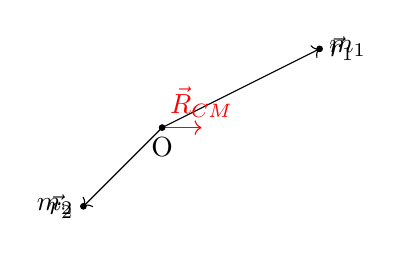
\begin{tikzpicture}
\draw[->] (0,0) -- (2,1) node[right] {$\vec{r}_1$};
\draw[->] (0,0) -- (-1,-1) node[left] {$\vec{r}_2$};
\draw[red,->] (0,0) -- (0.5,0) node[above] {$\vec{R}_{CM}$};
\draw[fill] (2,1) circle (1pt) node[right] {$m_1$};
\draw[fill] (-1,-1) circle (1pt) node[left] {$m_2$};
\draw[fill] (0,0) circle (1pt) node[below] {O};
\end{tikzpicture}
\end{center}
Dazu führen wir Schwerpunkts- und Relativkoordinaten ein:

$\vec{R}_{CM} = \frac{m_1\vec{r}_1 + m_2\vec{r}_2}{m_1+m_2}$, $\vec{r}=\vec{r}_1-\vec{r}_2$

$\Rightarrow \mu \ddot{\vec{r}} = \vec{F}_{12}$, $\mu = \frac{m_1m_2}{m_1+m_2} = \text{reduzierte Masse}$

Für den erhaltenen Drehimpuls haben wir dann den folgenden
Ausdruck herableiten: (Siehe Mech I - Skript S. 238)

$\vec{L} = \mu \vec{r} \times \dot{\vec{r}}$, $\frac{d\vec{L}}{dt} = 0$

Wir können unser Koordinatensystem so legen dass die z-Achse in Richtung von $\vec{L}$ zeigt:

$\vec{L} = L_z \vec{e}_z$, $L_z = \mu r^2\dot{\phi}$ in Polarkoordinaten.

Für die effektive Gesamtenergie ergibt sich der folgende Ausdruck:

$E = \frac{\mu}{2}\dot{r}^2 + U_{eff}(r)$, $U_{eff}(r) = V(r) + \frac{L^2}{2\mu r^2}$

Schließlich erinnern wir noch an unsere Formel für die Bahnkurve in Polarkoordinaten (Mech I-Skript, S.241):

$\phi - \phi_0 = \pm \frac{L}{\sqrt{2\mu}} \int_{r_0}^r \frac{dr'}{r'\sqrt{E-U_{eff}(r')}}$

Aus der Form des effektiven Potentials $U_{eff}(r)$ kann man die qualitative Form der Bewegung leicht ablesen.

\begin{center}
\begin{tikzpicture}[scale=0.8]
\draw[->] (-1,0) -- (6,0) node[right] {$r$};
\draw[->] (0,-1) -- (0,4) node[above] {Energie};
\draw[domain=1:6, smooth] plot (\x,{4/(\x*\x) - 2/\x});
\draw[red] (-1,2) -- (6,2) node[right] {$E>0$};
\node at (1.5,-0.3) {$r_{min}$};
\draw (0,0) node[left] {$0$};
\end{tikzpicture}
\end{center}
Falls $U(r) \to 0$ für $r \to \infty$, gibt es für $E > 0$ eine ungebundene Bewegung im Zwei-Körperproblem: Das (fiktive) Teilchen der Masse $\mu$ läuft aus dem Unendlichen auf das Potentialzentrum zu, erreicht einen minimalen Abstand $r_{min}$ und läuft dann wieder ins Unendliche weg. Dabei wird das Teilchen um einen Winkel $\Theta$ abgelenkt. Eine solche Bewegung wird ``Streuung'' bezeichnet.

\textbf{Beispiele:}
\begin{itemize}
\item Stoß eines Billardkugel
\item Ablenkung eines Kometen im Gravitationsfeld der Sonne
\item Ablenkung eines $\alpha$-Teilchens im Coulombfeld eines Atomkerns
\end{itemize}

Im ersten Teil dieser Vorlesung wollen wir das Problem der Streuung im Rahmen der klassischen Mechanik untersuchen.
\subsection{Kapitel 1: Klassische Streutheorie}

Die Streuung von Teilchen aneinander spielt bei der Erforschung der Materie eine wichtige Rolle: in vielen Teilchenbeobachtungen werden Elementarteilchen aufeinander geschossen und aneinander gestreut. Um die nötigen Konzepte zur Beschreibung von Streuexperimenten kennenzulernen, wollen wir uns hier mit Teilchenstreuung im klassischen Grenzfall beschäftigen, wo die Teilchen nicht-relativistisch und nicht-quantenmechanisch behandelt werden.

\subsubsection{Wirkungsquerschnitt}

Der typische Aufbau eines Streuexperiments sieht so aus:

\begin{center}
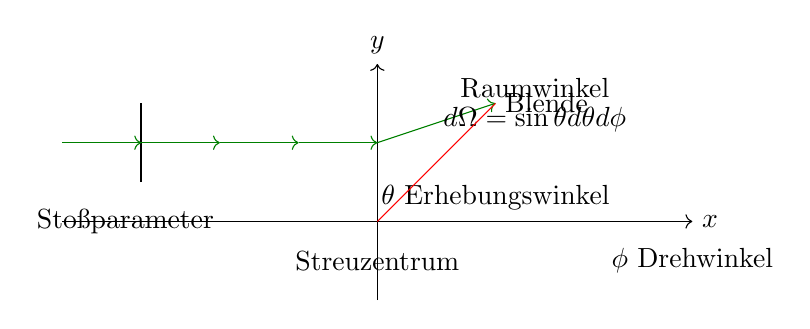
\begin{tikzpicture}
\draw[->] (-4,0) -- (4,0) node[right] {$x$};
\draw[->] (0,-1) -- (0,2) node[above] {$y$};
\draw[thick] (-3,0.5) -- (-3,1.5);
\draw[green!50!black, ->] (-4,1) -- (-3,1);
\draw[green!50!black, ->] (-3,1) -- (-2,1);
\draw[green!50!black, ->] (-2,1) -- (-1,1);
\draw[green!50!black, ->] (-1,1) -- (0,1);
\draw[green!50!black, ->] (0,1) -- (1.5,1.5);
\draw (2,1.7) node {Raumwinkel};
\draw (2,1.3) node {$d\Omega=\sin\theta d\theta d\phi$};
\draw (-3.2,0) node {Stoßparameter};
\draw (0,-0.5) node {Streuzentrum};
\draw (1.5,0.3) node {$\theta$ Erhebungswinkel};
\draw (4,-0.5) node {$\phi$ Drehwinkel};
\draw[red] (0,0) -- (1.5,1.5);
\draw (1.5,1.5) node[right] {Blende};
\end{tikzpicture}
\end{center}

Ein Strom gleich artiger Teilchen (Projektile) läuft auf eine Ansammlung ruhender Teilchen (Target) zu. Wenn jedes Projektil maximal mit einem Targetteilchen wechselwirkt, lässt sich dieser Vorgang als Zwei-Körper-Problem beschreiben. Wir betrachten zunächst das entsprechende effektive Ein-Körper Problem.
\subsubsection{Vor Streuung}

\begin{itemize}
\item alle Teilchen im Strahl haben die gleiche Geschwindigkeit $\vec{v}(\infty)$ und die gleiche Energie $E = \frac{\mu}{2}\vec{v}^2(\infty)$.

\item der Teilchenstrom ist durch homogene Teilchenstromdichte $j_0$ charakterisiert:

\[
j_0 = \frac{N_0}{A} = \frac{\text{Anzahl der auf Fläche A in Zeit T}\text{ einfallenden Teilchen}}{(\text{Zeit T}) \cdot (\text{Fläche A})}
\]

\item jedes Projektil ist durch seinen Abstand s von der Strahlachse charakterisiert, den sog. Stoßparameter.
\end{itemize}

\subsubsection{Nach Streuung}

Der Detektor registriert im Raumwinkel $d\Omega$ eine gewisse Zählrate $dN(\hat{\Omega})$ (d.h. Anzahl der in $d\Omega$ gezählten Teilchen pro Zeiteinheit). Die Zählrate entspricht einem Teilchenstrom

\[
dJ(\hat{\Omega}) = dN(\hat{\Omega}),
\]

der in die durch den Einheitsvektor $\hat{\Omega}(\theta,\phi)$ definierte Richtung fließt. Um ein Maß für die Stärke der Streuung zu erhalten, muß man den in $d\Omega$ gemessenen Teilchenstrom $dJ(\hat{\Omega})$ auf die einfallende Stromdichte normieren und durch den Raumwinkel $d\Omega$ teilen:

\[
\sigma(\hat{\Omega}) = \frac{dJ(\hat{\Omega})}{d\Omega j_0} = \frac{dN(\hat{\Omega})}{d\Omega j_0} = \text{differenzieller Wirkungsquerschnitt.}
\]
Offenbar hat $\sigma(\hat{\Omega})$ die Einheiten einer Fläche. Summieren wir die Beiträge von allen Richtungen auf, so erhalten wir den sogenannten totalen Wirkungsquerschnitt:

\[
\sigma_{tot} = \int d\Omega\: \sigma(\hat{\Omega}) = \int_0^{2\pi} d\phi \int_0^{\pi} d\theta\sin\theta\: \sigma(\theta,\phi)
\]

Die Gesamtzahl der gestreuten Teilchen ist somit $N_{tot} = \sigma_{tot} j_0$. Intuitiv kann man $\sigma_{tot}$ als effektive Querschnittsfläche interpretieren, die das Potential dem Projektil bietet. Das wird am Beispiel der Streuung an einer harten Kugel deutlich:

\begin{center}
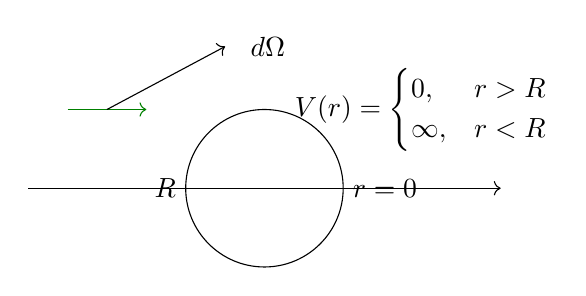
\begin{tikzpicture}
\draw[->] (-3,0) -- (3,0);
\draw[green!50!black,->] (-2.5,1) -- (-1.5,1);
\draw (0,0) circle (1);
\draw (1,0) node[right] {$r=0$};
\draw (-1,0) node[left] {$R$};
\node at (2,1) {$V(r)=\begin{cases} 0, & r>R \\ \infty, & r<R \end{cases}$};
\draw[->] (-2,1) -- (-0.5,1.8);
\draw (-0.3,1.8) node[right] {$d\Omega$};
\end{tikzpicture}
\end{center}

In Übungsaufgabe 1 wird gezeigt dass in diesem Fall
\[
\sigma_{tot} = \pi R^2 = \text{Querschnittsfläche der Kugel.}
\]

Man beachte, dass die hier eingeführten Definitionen unabhängig davon gelten, ob die Streuung klassisch oder quantenmechanisch beschrieben wird, oder ob die Streuung elastisch (ohne Energieaustausch) oder inelastisch erfolgt.

\subsubsection{Berechnung des Wirkungsquerschnitts für elastische Streuung am Zentralpotential}

Wir wollen nun den Wirkungsquerschnitt unter den folgenden Annahmen explizit berechnen:

\begin{enumerate}
\item Die Streuung kann im Rahmen der klassischen Mechanik beschrieben werden.
\item Die Streuung ist elastisch (d.h. kein Energie austausch zwischen Projektil und Target, der zur inneren Anregung führt; keine Teilchenproduktion bei relativistischen Vorgängen).
\item Die Streuung erfolgt am Zentralpotential $V(\vec{r})=V(|\vec{r}|)$ (d.h. das zwischen Projektil und Target wirkende Potential hängt nur vom Betrag des Abstands ab).
\end{enumerate}

Für ein repulsives Potential sieht dann die Trajektorie des Projektils im effektiven Einkörperproblem etwa so aus:

\begin{center}
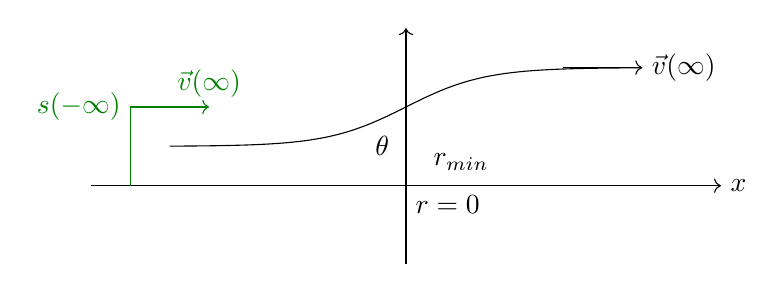
\begin{tikzpicture}
\draw[->] (-4,0) -- (4,0) node[right] {$x$};
\draw[->] (0,-1) -- (0,2);
\draw[green!50!black, ->] (-3.5,1) -- (-2.5,1) node[above] {$\vec{v}(\infty)$};
\draw[green!50!black] (-3.5,0) -- (-3.5,1) node[left] {$s(-\infty)$};
\draw[->] (2,1.5) -- (3,1.5) node[right] {$\vec{v}(\infty)$};
\draw (0,0) node[below right] {$r=0$};
\draw (0.7,0.3) node {$r_{min}$};
\draw (-0.3,0.5) node {$\theta$};
\draw[domain=-3:3, smooth] plot (\x,{1+0.5*tanh(\x)});
\end{tikzpicture}
\end{center}

Wir legen die Bahnkurve in x-y-Ebene, sodaß der erhaltene Drehimpuls von der Form $\vec{L}=L_z\vec{e}_z$ ist.
Wir leiten zunächst einen Zusammenhang zwischen dem differentiellen Wirkungsquerschnitt $\sigma(\hat{\Omega})$ und dem Stoßparameter $s$ her. Ausgangspunkt dafür sind die Erhaltungssätze:

Energieerhaltung:
\[
E(-\infty) = \frac{1}{2}\mu\vec{v}^2(-\infty) = E(\infty) = \frac{1}{2}\mu\vec{v}^2(\infty) \Rightarrow |\vec{v}(-\infty)| = |\vec{v}(\infty)|
\]

Drehimpulserhaltung:
\[
L_z(-\infty) = \mu v(-\infty)s(-\infty) = L_z(\infty) = \mu v(\infty)s(\infty) \Rightarrow s(-\infty) = s(\infty) = s
\]

Aus $L=L_z = \mu v(\infty)s$ und $E = \frac{\mu}{2}v^2(\infty)$ folgt der Zusammenhang zwischen Stoßparameter $s$, Energie und Drehimpuls im Streuzentrum:

\[
L = s\sqrt{2\mu E}
\]

Für den in der Skizze eingezeichneten Streuwinkel $\theta$ können wir schreiben:
$\theta = \pi - 2\psi_{\infty}$. Für ein Zentralpotential hängt der Streuwinkel aus Symmetriegründen nur vom Abstand $s$ des Projektils von der Strahlachse und der Energie (und nicht vom Drehwinkel $\phi$) ab:

\[
\theta = \theta(s,E) \Rightarrow s = s(\theta,E)
\]

Aus demselben Grund ist $\sigma(\hat{\Omega}) = \sigma(\theta)$ unabhängig von $\phi$. 
Unsere Strategie ist, den Stoßparameter $s = s(\theta,E)$ als Funktion von Streuwinkel $\theta$ und Energie $E$ durch Lösung der Bahnkurve zu bestimmen. Aus $s(\theta,E)$ lässt sich $\sigma(\theta,E)$ leicht berechnen:


Zusammenhang zwischen $\sigma(\theta,E)$ und $s(\theta,E)$:

Dazu betrachten wir die Bilanzgleichung die beschreibt dass bei der Streuung kein Teilchen verlorengeht.

\begin{center}
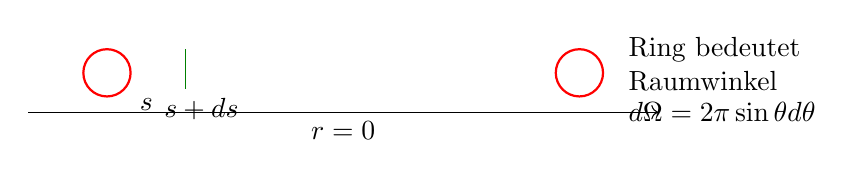
\begin{tikzpicture}
\draw[->] (-4,0) -- (4,0);
\draw[red,thick] (-3,0.5) circle (0.3);
\draw[red,thick] (3,0.5) circle (0.3);
\draw[green!50!black] (-2,0.3) -- (-2,0.8);
\draw (0,0) node[below] {$r=0$};
\draw (-2.5,0.3) node[below] {$s$};
\draw (-1.8,0.3) node[below] {$s+ds$};
\draw (3.5,0.8) node[right] {Ring bedeutet};
\draw (3.5,0.4) node[right] {Raumwinkel};
\draw (3.5,0) node[right] {$d\Omega=2\pi\sin\theta d\theta$};
\end{tikzpicture}
\end{center}

man beachte: $\frac{ds}{d\theta} < 0$ für repulsives Potential

Bilanzgleichung:

$$
\begin{aligned}
j_0 2 \pi s|d s| &= dN'(\Omega) = \sigma(\theta) j_0 \ln \sin \theta|d \theta| \\
\text{Zahl der pro Zeiteinheit} & \hspace{2cm} \text{Zahl der in Raumwinkel} \\
\text{durch Kreisring } 2\pi s|ds| & \hspace{2cm} d\Omega=2\pi\sin\theta |d\theta| \text{ pro Zeit-} \\
\text{anlaufenden Teilchen.} & \hspace{2cm} \text{einheit gestreuten Teilchen} \\[1ex]
\Rightarrow \sigma(\theta,E) &= \frac{s(\theta,E)}{\sin\theta} \left|\frac{ds(\theta,E)}{d\theta}\right|
\end{aligned}
$$
Um den differentiellen Wirkungsquerschnitt zu berechnen, müssen wir also bei fester Energie $E$ den Stoßparameter $s(\theta,E)$ als Funktion des Streuwinkels bestimmen.



\subsubsection{Berechnung von $S=S(\theta,E)$:}

\begin{center}
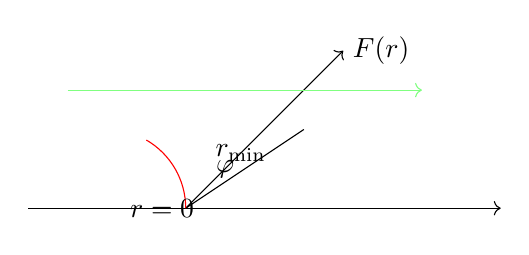
\begin{tikzpicture}
\draw[->] (-2,0) -- (4,0);
\draw[->] (0,0) -- (2,2) node[right] {$F(r)$};
\draw[green!50, ->] (-1.5,1.5) .. controls (0,1.5) and (1.5,1.5) .. (3,1.5);
\draw (0,0) -- (1.5,1);
\draw[red] (0,0) arc (0:60:1);
\node at (0.5,0.5) {$\varphi$};
\node at (-0.3,0) {$r=0$};
\node at (0.7,0.7) {$r_{\text{min}}$};
\end{tikzpicture}
\end{center}

Gegeben: beliebiges Zentralpotential $V(r)$, $V_{\text{eff}}(r)=V(r)+\frac{L^2}{2\mu r^2}$

Wir legen unser Koordinatensystem so, dass der Punkt minimaler Annäherung der Projektile an das Target dem Winkel $\varphi=0$ entspricht (siehe Skizze). Aus der expliziten Formel für die Bahnkurve im Zentralpotential (siehe S.5, mit $\varphi_0=0$ und $r_0=r_{\text{min}}$) folgt dann:

\[ \varphi(r,L,E)= \frac{L}{\sqrt{2\mu}} \int_{r_{\text{min}}}^r \frac{dr'}{r'^2\sqrt{E-V_{\text{eff}}(r')}} \]

Dabei ist $r_{\text{min}}$ Nullstelle der Gleichung $E-V_{\text{eff}}(r)=0$.

\[ \Rightarrow \theta(L,E) = \pi - 2\varphi(\infty,L,E) \]
\[ = \pi - \frac{2L}{\sqrt{2\mu}} \int_{r_{\text{min}}}^\infty \frac{dr'}{r'^2\sqrt{E-V_{\text{eff}}(r')}} \]

Mit $L = S\sqrt{2\mu E}$ (siehe S.16) erhalten wir dann durch Einsetzen die Funktion $\theta = \theta(S,E)$ und durch Auflösen nach $S$ die gesuchte Funktion $S=S(\theta,E)$.


\subsubsection{Beispiel: Rutherford'scher Wirkungsquerschnitt}

Rutherford, 1913: Streuung von positiv geladenen Atomkernen.\\
Projektile: He-Atomkerne ($\alpha$-Teilchen). Ladung $Z_1e=2e$,\\
Energie: $E \approx 4$ bis $8\text{ MeV}$ (natürliche Radioaktivität)\\
Target: Goldfolie: Ladung der Kerne: $Z_2e=79e$.

$\Rightarrow$ Streuung am repulsiven Coulomb-Potential:
\[ V(r) = \frac{k}{r}, \quad k = Z_1Z_2e^2. \]

Durch direktes Ausführen des Integrals auf S.11 (oder eleganter mit Hilfe des Runge-Lenz-Vektors, siehe Übung auf Seite) erhalten wir für den Winkel $\varphi_\infty = \varphi(r=\infty,L,E)$:

\[ \cos\varphi_\infty = \frac{k}{2SE}\frac{1}{\sqrt{1+\frac{k^2}{4S^2E^2}}} = \frac{k}{\sqrt{k^2+4S^2E^2}} \]

\[ \Rightarrow S^2 = \frac{k^2}{4E^2}\left(\frac{1}{\cos^2\varphi_\infty}-1\right) = \frac{k^2}{4E^2}\tan^2\varphi_\infty \]

Mit $\varphi_\infty = \frac{\pi}{2} - \frac{\theta}{2}$, $\tan^2\varphi_\infty = \cot^2(\frac{\theta}{2})$

\[ \Rightarrow \sigma(\theta,E) = \frac{S(\theta,E)}{\sin\theta}\left|\frac{dS(\theta,E)}{d\theta}\right| = \frac{1}{2\sin\theta}\left|\frac{d}{d\theta}S^2(\theta,E)\right| \]
\[ = \frac{k^2}{8E^2}\frac{1}{\sin\theta}\left|\frac{d}{d\theta}\cot^2(\frac{\theta}{2})\right| \]

mit 
$$\frac{d}{d\theta}\cot^2\frac{\theta}{2} = 2\cot\frac{\theta}{2}\frac{d}{d\theta}(\cot\frac{\theta}{2}) = \cot\frac{\theta}{2}\frac{1}{\sin^2\frac{\theta}{2}} = \frac{\cos(\frac{\theta}{2})}{\sin^3\frac{\theta}{2}}$$
Mit $\sin\theta = 2\sin\frac{\theta}{2}\cos\frac{\theta}{2}$ erhalten wir schließlich:

\[\sigma(\theta,E) = \frac{k^2}{16E^2}\frac{1}{\sin^4\frac{\theta}{2}} = \left(\frac{Z_1Z_2e^2}{4E}\right)^2\frac{1}{\sin^4\frac{\theta}{2}}\]
``Rutherfordscher Wirkungsquerschnitt''

\noindent\textbf{Anmerkungen:}

\begin{enumerate}
\item Für kleine Streuwinkel $\theta$ (d.h. große Stoßparameter) divergiert der Rutherfordsche Wirkungsquerschnitt wie
\[\sigma(\theta,E) \sim \left(\frac{Z_1Z_2e^2}{E^2\theta^4}\right)^2\]

\item $\Rightarrow \sigma_{\text{tot}} = \infty$. Man sagt: das Coulomb-Potential hat unendliche Reichweite.

\item Eine quantenmechanische Berechnung des Wirkungsquerschnitts für das Coulomb-Potential liefert erstaunlicherweise genau dasselbe Ergebnis wie unsere klassische Rechnung!

\item Bei $\theta = 0$ (Vorwärtsstreuung) kann $\sigma(\theta,E)$ nicht gemessen werden, da dies die Stelle nicht gibt. Im tatsächlichen Experiment wird das Coulomb-Potential durch die negativ geladenen Elektronen der Atomhülle abgeschirmt, so dass $\alpha$-Teilchen mit Stoßparameter der größer als der Radius der Atomhülle ist keine Ablenkung mehr erfahren.

\end{enumerate}


\subsubsection{Rücktransformation ins Laborsystem}

Nach der Reduktion des Zweikörperproblems auf ein effektives Einkörperproblem kann die Relativbewegung so diskutiert werden, als ob ein fiktives Teilchen der Masse $\mu=\frac{m_1m_2}{m_1+m_2}$ sich im Potential $V(r)$ bewegt - in diesem Bild haben wir den Wirkungsquerschnitt hergeleitet. Die Ergebnisse wollen wir nun wieder für das zugrunde liegende Zweikörperproblem formulieren.

Laborsystem

Der Experimentator misst den Wirkungsquerschnitt von seinem Laborsystem aus, wo das Targetteilchen vor dem Stoß in Ruhe ($\vec{v}_2(t<0)=0$) ist. Die Trajektorien von Projektil und Target sehen im Laborsystem typischerweise so aus:

\begin{center}
\begin{tikzpicture}
\draw[->] (-3,-2) -- (3,-2);
\draw[->] (-2,-3) -- (-2,0);
\draw[green!50,->] (-2,0) .. controls (0,1) and (2,1.5) .. (3,2);
\draw[red,->] (-2,-2) -- (3,-1);
\draw[dashed] (-2,0) -- (-2,-2);
\node at (-2.5,-1) {$s$};
\node[left] at (-2,0) {$m_1$ (Projektil)};
\node[left] at (-2,-2) {$m_2$ (Target)};
\draw (-1,0) arc (0:30:1);
\node at (-0.5,0.3) {$\theta_1$};
\draw (-1,-2) arc (0:15:1);
\node at (-0.5,-1.7) {$\theta_2$};
\end{tikzpicture}
\end{center}

Der Streuwinkel $\theta_1$ des Projektils im Laborsystem ist die experimentell zugängliche Größe.
Wegen Impulserhaltung (Schwerpunkt Satz) gilt im Laborsystem:
\[ m_1\vec{v}_1(-\infty) + m_2\vec{v}_2(-\infty) = m_1\vec{v}_1(0) + m_2\vec{v}_2(0) = M\vec{R}_{CM}, \quad M = m_1+m_2 \]

Da das Target vor dem Stoß ruht ($\vec{v}_2(-\infty)=0$)
\[ \Rightarrow \vec{R}_{CM} = \frac{m_1\vec{v}_1(0) + m_2\vec{v}_2(0)}{m_1+m_2} = \frac{m_1}{m_1+m_2}\vec{v}_1(-\infty) \]

\textbf{Spezial:} Zusammenhang zwischen $\theta_1$ und Streuwinkel des effektiven Einkörperproblems.

Dazu betrachten wir den Streuprozess im 
\textbf{Schwerpunktsystem:} (CMS = ``center of mass system'').

Ortsvektoren im CMS:
\[ \vec{r}_1' = \vec{r}_1 - \vec{R}_{CM} = \vec{r}_1 - \frac{m_1\vec{r}_1+m_2\vec{r}_2}{m_1+m_2} = \frac{m_2}{m_1+m_2}\vec{r} \]
\[ \vec{r}_2' = \vec{r}_2 - \vec{R}_{CM} = -\frac{m_1}{m_1+m_2}\vec{r} \]

\begin{center}
\begin{tikzpicture}
\draw[->] (-4,0) -- (4,0);
\draw (0,-3) -- (0,3);
\draw[green!50,->] (-3,2) -- (2,2);
\draw[green!50,dashed] (-3,2) -- (2,2);
\draw[red,->] (-3,-2) -- (2,-2);
\draw[red,dashed] (-3,-2) -- (2,-2);
\draw[thick] (-1,1) -- (1,-1);
\node at (-1,1) {$m_1$};
\node at (1,-1) {$m_2$};
\node at (-3.5,2) {$\vec{v}_1'(-\infty)$};
\node at (-3.5,-2) {$\vec{v}_2'(-\infty)$};
\node at (2.5,2) {$\vec{v}_1'(\infty)$};
\node at (2.5,-2) {$\vec{v}_2'(\infty)$};
\draw (0,0) -- (2,0) arc (0:30:2);
\node at (1.5,0.5) {$\theta$};
\draw[<->] (-1,1) -- (-1,0);
\node at (-1.3,0.5) {$s$};
\node at (0,-3.5) {V2 WS2025};
\node at (0.5,-3.5) {W/1};
\end{tikzpicture}
\end{center}


Da im CMS die Bewegung der einzelnen Massen direkt mit dem Relativvektor $\vec{r}=\vec{r}_1-\vec{r}_2$ verknüpft ist, kann der Streuwinkel $\Theta$ des Projektils im CMS mit dem Streuwinkel $\theta$ des effektiven Einkörperproblems identifiziert werden.

Zur Berechnung des Streuwinkels des Projektils im Laborsystem $\theta_1 = \theta_1(\Theta)$ als Funktion von $\Theta$ benötigen wir die asymptotische Geschwindigkeit $\vec{v}_1'(\infty)$ im CMS, die mit der entsprechenden Geschwindigkeit $\vec{v}_1'(\infty)$ im Laborsystem über

\[\vec{v}_1'(\infty) = \vec{v}_1'(\infty) - \vec{R}_{CM}\]

zusammenhängt:

aus der Skizze ergibt sich
\[\tan\theta_1 = \frac{v_1'(\infty)\sin\Theta}{v_1'(\infty)\cos\Theta + |\vec{R}_{CM}|}\]

\[= \frac{\sin\Theta}{\cos\Theta + \frac{|\vec{R}_{CM}|}{v_1'(\infty)}}\]

Da das Target im Laborsystem vor dem Stoß ruht, bewegt es sich im CMS vor dem Stoß mit $-\vec{R}_{CM}$ auf den Ursprung zu, d.h.

\[\vec{v}_2'(-\infty) = -\vec{R}_{CM}\]

\[\Rightarrow \tan\theta_1 = \frac{\sin\Theta}{\cos\Theta + \frac{v_2'(-\infty)}{v_1'(\infty)}}\]

Zur weiteren Umformung des Geschwindigkeitsverhältnisses im Nenner benutzen wir dass im CMS die Summe der Impulse der Teilchen verschwindet:
\[\vec{R}_{CM}' = 0 = m_1\vec{v}_1' + m_2\vec{v}_2'\]
\[\vec{v}_2'(+\infty) = -\frac{m_1}{m_2}\vec{v}_1'(+\infty), \quad \vec{v}_2'(-\infty) = -\frac{m_1}{m_2}\vec{v}_1'(-\infty)\]

\[\Rightarrow \frac{v_2'(-\infty)}{v_1'(\infty)} = \frac{v_2'(-\infty)}{v_1'(-\infty)}\cdot\frac{v_1'(-\infty)}{v_1'(\infty)} = \frac{m_1}{m_2}\cdot\frac{v_1'(\infty)}{v_1'(\infty)}\]

Im CMS bleiben aber wegen Energieerhaltung die Beträge der asymptotischen Geschwindigkeiten vor und nach dem Stoß konstant, d.h.

\[v_1'(-\infty) = v_1'(\infty), \quad v_2'(-\infty) = v_2'(\infty)\]

Formal sieht man das so: Da U(r) endliche Reichweite hat, besteht die Gesamtenergie $E'$ im CMS vor und nach dem Stoß nur aus kinetischer Energie:

Vor Stoß:
\[E' = \frac{m_1}{2}v_1'^2(-\infty) + \frac{m_2}{2}v_2'^2(-\infty)\]
\[= \frac{m_1}{2}v_1'^2(-\infty)\left(1+\frac{m_1}{m_2}\right) = \frac{m_2}{2}v_2'^2(-\infty)\left(1+\frac{m_2}{m_1}\right)\]

nach Stoß:
\[E' = \frac{m_1}{2}v_1'^2(\infty) + \frac{m_2}{2}v_2'^2(\infty)\]
\[= \frac{m_1}{2}v_1'^2(\infty)\left(1+\frac{m_1}{m_2}\right) = \frac{m_2}{2}v_2'^2(\infty)\left(1+\frac{m_2}{m_1}\right)\]

Insgesamt ergibt sich somit für das benötigte Geschwindigkeitsverhältnis:

\[\frac{v_2'(\infty)}{v_1'(\infty)} = \frac{m_1}{m_2}\cdot\frac{v_1'(-\infty)}{v_1'(\infty)} = \frac{m_1}{m_2}\]

\[\Rightarrow \tan\theta_1 = \frac{\sin\Theta}{\cos\Theta + \frac{m_1}{m_2}}\]

Zusammenhang zwischen Streuwinkel $\theta_1$ im Laborsystem und Streuwinkel $\Theta$ des effektiven Einkörperproblems.
\section*{Grenzfälle:}

\begin{enumerate}
\item $\frac{m_1}{m_2} \to 0$ (infinitesimal schweres Target) $\Rightarrow \theta_1 = \Theta$

\item $\frac{m_1}{m_2} = 1$ (gleich schwere Teilchen): $\tan \theta_1 = \frac{\sin \Theta}{\cos \Theta + 1} = \tan \frac{\Theta}{2}$

$\Rightarrow \theta_1 = \frac{\Theta}{2}$, d.h. Streuung nach Rückwärts im CMS ($\Theta = \pi$) erscheint als Streuung um $\frac{\pi}{2}$ im Laborsystem.
\end{enumerate}

Allgemein gilt $\theta_1 < \Theta$, d.h. die Streuung im Laborsystem erscheint mehr in Vorwärtsrichtung gebündelt als im CMS.

Schließlich wollen wir noch den differentiellen Wirkungsquerschnitt $\sigma(\Theta)$ im CMS in den entsprechenden Wirkungsquerschnitt $\sigma_L(\theta_1)$ im Laborsystem umrechnen. Die durch einen Kreisring $2\pi S dS$ einlaufende Teilchenzahl pro Zeiteinheit bleibt dieselbe, da der Stoßparameter $S$ in beiden Systemen derselbe ist - die Teilchen werden nur in verschiedene Raumwinkel gestreut. Somit muss gelten:

\[\sigma(\Theta) 2\pi \sin \Theta d\Theta = \sigma_L(\theta_1) 2\pi \sin \theta_1 d\theta_1\]

\[\Rightarrow \sigma_L(\theta_1) = \sigma(\Theta) \frac{\sin \Theta d\Theta}{\sin \theta_1 d\theta_1} = \sigma(\Theta) \frac{d(\cos \Theta)}{d(\cos \theta_1)}\]

Zur Berechnung der Ableitung lösen wir in $\tan \theta_1 = \frac{\sin \Theta}{\cos \Theta + \frac{m_1}{m_2}}$ cos $\theta_1$ als Funktion von cos $\Theta$ auf.

Mit $\tan \theta_1 = \frac{\sin \theta_1}{\cos \theta_1} = \frac{\sqrt{1-\cos^2\theta_1}}{\cos \theta_1}$, $\sin \Theta = \sqrt{1-\cos^2\Theta}$

\[\Rightarrow \cos \Theta = -\frac{m_1}{m_2}(1-\cos^2\theta_1) + \cos \theta_1 \sqrt{1-(\frac{m_1}{m_2})^2(1-\cos^2\theta_1)}\]

(siehe Nebenrechnung!)
\[\frac{d(\cos\Theta)}{d(\cos\theta_1)} = 2\frac{m_1}{m_2}\cos\theta_1 + \frac{1-(\frac{m_1}{m_2})^2+2(\frac{m_1}{m_2})^2\cos^2\theta_1}{\sqrt{1-(\frac{m_1}{m_2})^2\sin^2\theta_1}}\]

Im Besondere ergibt sich für den wichtigen Spezialfall $m_1=m_2$ mit $\theta_1=\frac{\Theta}{2}$ der Zusammenhang zwischen den Wirkungsquerschnitten

\[\sigma_L(\theta_1)=\sigma(2\theta_1)=4\cos\theta_1\]


\subsubsection{Nebenrechnung:}

\begin{align*}
\tan\theta_1 &= \frac{\sin\theta_1}{\cos\theta_1} = \frac{\sin\Theta}{\cos\Theta + \frac{m_1}{m_2}} \\[2ex]
\Rightarrow \frac{\sqrt{1-\cos^2\theta_1}}{\cos\theta_1} &= \frac{\sqrt{1-\cos^2\Theta}}{\cos\Theta + \frac{m_1}{m_2}} \\[2ex]
\Rightarrow \frac{1-\cos^2\theta_1}{\cos^2\theta_1} &= \frac{1-\cos^2\Theta}{(\cos\Theta + \frac{m_1}{m_2})^2} \\[2ex]
\Rightarrow (\cos\Theta + \frac{m_1}{m_2})^2(1-\cos^2\theta_1) &= \cos^2\theta_1(1-\cos^2\Theta) \\[2ex]
\Rightarrow \cos^2\Theta + 2\cos\Theta\frac{m_1}{m_2} + (\frac{m_1}{m_2})^2(1-\cos^2\theta_1) &= \cos^2\theta_1(1-\cos^2\Theta) \\[2ex]
\Rightarrow \cos^2\Theta(1-\cos^2\theta_1 + \cos^2\theta_1) &+ 2\cos\Theta\frac{m_1}{m_2}(1-\cos^2\theta_1) \\
&+ (\frac{m_1}{m_2})^2(1-\cos^2\theta_1) = 0 \\[2ex]
\Rightarrow \cos^2\Theta + 2\cos\Theta\frac{m_1}{m_2}(1-\cos^2\theta_1) &+ (\frac{m_1}{m_2})^2(1-\cos^2\theta_1)(1+(\frac{m_1}{m_2})^2) = 0
\end{align*}
\[\cos\Theta = -\frac{m_1}{m_2}(1-\cos^2\theta_1)\]

\[\pm \sqrt{\left(\frac{m_1}{m_2}\right)^2(1-\cos^2\theta_1)^2 + \cos^2\theta_1\left(1+\left(\frac{m_1}{m_2}\right)^2\right)-\left(\frac{m_1}{m_2}\right)^2}\]

\[= -\frac{m_1}{m_2}(1-\cos^2\theta_1)\]

\[\pm \sqrt{\left(\frac{m_1}{m_2}\right)^2(1-2\cos^2\theta_1+\cos^4\theta_1) + \cos^2\theta_1\left(\frac{m_1}{m_2}\right)^2\cos^2\theta_1\left(\frac{m_1}{m_2}\right)^2}\]

\[= -\frac{m_1}{m_2}(1-\cos^2\theta_1 + \cos\theta_1\sqrt{1-\left(\frac{m_1}{m_2}\right)^2(1-\cos^2\theta_1)})\]



\pagebreak



\section{Teil II: Lagrange'sche Mechanik}
\vspace{0.3cm}
\noindent (Lagrange: frz. Mathematiker, 1736-1813)

Die Newton'sche Bewegungsgleichung $\vec{p} = \vec{F}$ gilt in Vektorform nur in Inertialsystemen, während die Komponenten-Form $\frac{dp_i}{dt} = F_i$, $i=1,2,3$, nur in kartesischen Koordinatensystemen in Inertialsystemen gilt. In anderen Koordinatensystemen gilt es extra Terme auf der linken Seite; zum Beispiel haben für ebene Probleme in Zylinderkoordinaten die Newton'schen Bewegungsgleichungen die Form

\[m(\ddot{r}-r\dot{\phi}^2) = F_r, \quad F_r = \vec{e}_r \cdot \vec{F}\]
\[m(\ddot{r}\phi + 2\dot{r}\dot{\phi}) = F_{\phi}, \quad F_{\phi} = \vec{e}_{\phi} \cdot \vec{F}\]

(das folgt aus dem in Mechanik I, Skript S. 192, hergeleiteten Ausdruck für die Beschleunigung in ebenen Polarkoordinaten:

\[\vec{a} = (\ddot{r}-r\dot{\phi}^2)\vec{e}_r + (\underbrace{r\ddot{\phi} + 2\dot{r}\dot{\phi}}_{=\frac{1}{r}\frac{d}{dt}(r^2\dot{\phi})})\vec{e}_{\phi} \quad).\]

Inertialsysteme und kartesische Koordinatensysteme sind jedoch weder der bequemste noch der allgemeinste Ausgangspunkt zur Analyse und Lösung physikalischer Probleme: Probleme mit sphärischer Symmetrie formuliert man am besten in sphärischen Koordinaten, und Phänomene auf rotierenden Körpern (z.B. die Erde) beschreibt man am besten mit Hilfe rotierender Bezugssysteme. Daher ist es wünschenswert, eine allgemeinere Formulierung der Mechanik zu entwickeln, die zwar denselben physikalischen Inhalt wie $\vec{p}=\vec{F}$ hat, die aber nicht den Einschränkungen der Newton'schen Bewegungsgleichungen unterliegt. Die Lagrange'sche Formulierung der Mechanik hat die gewünschten Eigenschaften:

Durch geeignete Umschreibung der Newton'schen Bewegungsgleichungen erhält man eine Formulierung der Mechanik, die in beliebigen Koordinatensystemen, sowie in beliebigen beschleunigten Bezugssystemen dieselbe Form hat.

Man sagt: Die Lagrange'sche Formulierung der Mechanik ist \emph{kovariant} in Bezug auf beliebige differenzierbare Koordinatentransformationen im Konfigurationsraum (der 3N-dimensionale Raum der Positionen von N Teilchen).

\textbf{Wichtig:} Im Rahmen der klassischen Mechanik beschreibt die Lagrange'sche Formulierung dieselbe Physik wie die Newton'schen Gesetze!

\textbf{Vorteile von Lagrange:}

\begin{enumerate}
\item Im Lagrange-Formalismus ist es nicht nötig, physikalische Probleme zunächst in Inertialsystemen mit kartesischen Koordinaten zu formulieren, und erst dann zu ``geschickten'' Systemen überzugehen.

\item Die Lagrange'sche Bewegungsgleichung der Mechanik ist ein Spezialfall der sogenannten ``Euler-Lagrange-Gleichungen'' der Variationsrechnung, die unabhängig von der Mechanik aus einem Variationsprinzip hergeleitet werden kann.

\item Die Lagrange-Funktion L spielt auch in der Quantenmechanik eine wichtige Rolle; in diesem Sinne hat die Lagrange'sche Formulierung der Mechanik die
fundamentalere Formulierung der Quantenmechanik als die Schrödinger-Formulierung (``Quantenrevolution überlöst'', $\to$ Feynman'sche Formulierung der Quantenmechanik, Pfadintegrale).

\item Die Lagrange'schen Bewegungsgleichungen eignen sich besonders gut, um Zusammenhänge zwischen Symmetrien und Erhaltungsgrößen herauszuarbeiten: Symmetrien manifestieren sich in Invarianzen der Lagrangefunktion.
\end{enumerate}



\subsection{Zwangsbedingungen und das d'Alembert-Prinzip}

\subsubsection{Zwangsbedingungen}

Im Kontext der Klassischen Mechanik versteht man unter Zwangsbedingungen geometrische Nebenbedingungen die den Bewegungsablauf eines Körpers einschränken.

\textbf{Beispiel:} Perle auf gebogenem, rotierenden Draht:

Auf einem parabelförmig gebogenen Draht, der sich mit konstanter Winkelgeschwindigkeit $\omega$ um die z-Achse dreht, ist eine Perle aufgezogen.

Zwangsbedingungen in Zylinderkoordinaten:
\[\phi - \omega t = 0\]
\[z - ar^2 = 0\]

Das sind 2 geometrische Einschränkungen für die 3 Koordinaten $(r,\phi,z)$, so dass durch die Angabe einer einzigen Koordinate (z oder r) die Position der Perle vollständig festgelegt ist.

Offensichtlich werden in diesem Beispiel die mit den Zwangsbedingungen verbundenen geometrischen Einschränkungen am einfachsten in Zylinderkoordinaten beschrieben. Natürlich hätten wir auch kartesische Koordinaten $(x,y,z)$ wählen können, aber dann sehen die Zwangsbedingungen komplizierter aus:
\[\arctan(\frac{y}{x})-\omega t = 0, \quad z-a(x^2+y^2) = 0\]



\subsubsection{a) Generalisierte Koordinaten}

Allgemein können wir den Zustand eines N-Teilchen Systems im 3-dimensionalen Raum durch die 3N Kartesischen Koordinaten der einzelnen Teilchen beschreiben, die wir mit $x_1,...,x_{3N}$ durchnummerieren. Alternativ können wir aber auch andere Größen $q_1,...,q_{3N}$ benutzen, die den geometrischen Zwangsbedingungen sehr angepaßt sind. Alle Größen, die die Konfiguration einer mechanischen Anordnung kennzeichnen können, werden ``generalisierte Koordinaten'' genannt. Dabei wollen wir annehmen, dass zwischen den Kartesischen Koordinaten $x_1,...,x_{3N}$ und den generalisierten Koordinaten $q_1,...,q_{3N}$ ein Zusammenhang der Form

\[x_i = x_i(q_1,...,q_{3N},t), \quad i=1,...,3N\]

besteht, wobei die explizite Zeitabhängigkeit einen Übergang auf bewegte Koordinatensysteme ermöglicht. Die obige Transformation wird ``Punkttransformation'' genannt, weil sie Punkte in verschiedenen Koordinatensystemen aufeinander abbildet.

\subsubsection{b) Klassifizierung von Zwangsbedingungen}

Für ein System mit Zwangsbedingungen sind nicht alle 3N Koordinaten $q_1,...,q_{3N}$ voneinander unabhängig, so dass es Zusammenhänge zwischen den $q_i$ und eventuell auch zwischen den entsprechenden generalisierten Geschwindigkeiten $\dot{q}_i = \frac{d}{dt}q_i$ gibt. Man unterscheidet folgende Fälle: (wobei die $f_j(\dots)$ beliebige Funktionen der angegebenen Argumente sind):

\begin{tabular}{|l|l|l|}
\hline
 & skleronome & rheonome \\
 & (zeitunabhängig) & (zeitabhängig) \\
\hline
holonom & $f_j(q_1,...,q_{3N}) = 0,$ & $f_j(q_1,...,q_{3N},t) = 0$ \\
(ganz gestrickt) & $j = 1,...,k$ & \\
\hline
nicht- & $f_j(q_1,...,q_{3N}) \geq 0$ & $f_j(q_1,...,q_{3N},t) \geq 0$ \\
holonom & $f_j(q_1,...,q_{3N},\dot{q}_1,...,\dot{q}_{3N}) = 0$ & $f_j(q_1,...,q_{3N},\dot{q}_1,...,\dot{q}_{3N},t) = 0$ \\
\hline
\end{tabular}

Der Index $j = 1,...,k \leq 3N$ nummeriert die Zwangsbedingungen. $k$ unabhängige holonome ZB reduzieren die Zahl der Freiheitsgrade eines Systems von $N$ Massenpunkten in $D$ Dimensionen auf $DN-k$.

\textbf{Beispiele:}

1) Perle auf Draht, siehe S. 25: $N=1$, $D=3$, $k=2$
   
   $\Rightarrow 3N-2 = 1$ Freiheitsgrad;
   
   ZB $\phi - \omega t = 0$ ist holonom rheonom,
   
   ZB $r-a^2 = 0$ ist holonom skleronom.

2) Scheibe mit Radius R rollt ohne schlupf auf schiefer Ebene:

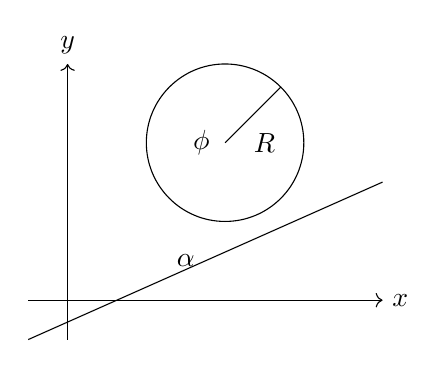
\begin{tikzpicture}
\draw[->] (-0.5,0) -- (4,0) node[right] {$x$};
\draw[->] (0,-0.5) -- (0,3) node[above] {$y$};
\draw (-0.5,-0.5) -- (4,1.5);
\draw (2,2) circle (1);
\draw (2,2) -- +(45:1);
\node at (1.5,0.5) {$\alpha$};
\node at (2.5,2) {$R$};
\node at (1.7,2) {$\phi$};
\end{tikzpicture}

Ohne ZBs würde die Lage der Scheibe durch 3 Koordinaten bestimmt,

ZB: $x_A, y_A, \phi$

2 holonome ZBs:

$x_A - R\phi \cos\alpha = 0$

$y_A - R\phi \sin\alpha = 0$


\subsubsection{c) Nicht-holonome Zwangsbedingungen}

Darunter versteht man alle ZB, die sich nicht auf Gleichungen der Form $f_j(q_1,...,q_M,t)=0$ zurückführen lassen, welche nur die generalisierten Koordinaten und die Zeit enthalten. (dabei ist M die maximal mögliche Zahl der generalisierten Koordinaten, $M=DN$ für N Teilchen in D Dimensionen).

Man unterscheidet zwei verschiedene Typen von nicht-holonomen ZB:

1) Ungleichungen:

Manche ZB lassen sich mathematisch nur als Ungleichungen formulieren.

\textbf{Beispiel:} Kleine Kugel rollt Oberfläche einer großen Kugel herunter:
ZB: $F(t) \geq R$

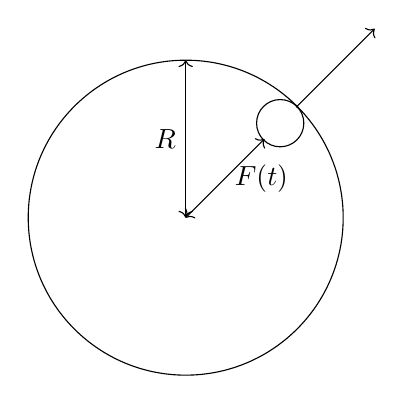
\begin{tikzpicture}
\draw (0,0) circle (2);
\draw[->] (1.4,1.4) -- (2.4,2.4);
\draw[<->] (0,0) -- (1,1) node[midway,right] {$F(t)$};
\draw[<->] (0,0) -- (0,2) node[midway,left] {$R$};
\draw (1.2,1.2) circle (0.3);
\end{tikzpicture}

Ist die Geschwindigkeit der kleinen Kugel groß genug, verliert sie wegen ihrer Zentrifugalkraft beim Herunterfallen den Kontakt zur großen Kugel.

2) Nicht-integrable Zwangsbedingungen:

Darunter versteht man ZB der Form

\[f_j(q_1,...,q_M,\dot{q}_1,...,\dot{q}_M,t) = 0\]

die sich nicht durch geeignete Integration in holonome ZB der Form $h_j(q_1,...,q_M,t)=0$ umwandeln lassen.
\textbf{26}

Um besser zu verstehen weshalb dies nicht immer geht, betrachten wir zunächst eine holonome ZB,

\[h_j(q_1,...,q_M,t) = 0\]

\[\Rightarrow \frac{d}{dt}h_j(q_1,...,q_M,t) = 0 = \sum_{i=1}^M \frac{\partial h_j}{\partial q_i}\dot{q}_i + \frac{\partial h_j}{\partial t} \equiv f_j(\dot{q}_1,...,\dot{q}_M,t)\]

Durch Ableiten einer holonomen ZB erhält man also eine ZB welche die Geschwindigkeiten $\dot{q}_i$ enthält. Wir können diese ZB auch in differentieller Form schreiben indem wir sie mit dt durchmultiplizieren und $dq_i = \dot{q}_i dt$ benutzen:

\begin{equation*}
\sum_{i=1}^M a_{ji}dq_i + a_{jt}dt = 0
\end{equation*}

mit \[a_{ji} = \frac{\partial h_j(q_1,...,q_M,t)}{\partial q_i}, \quad a_{jt} = \frac{\partial h_j(q_1,...,q_M,t)}{\partial t}\]

Da man (bei hinreichend glatten Funktionen) die Reihenfolge der zweiten Ableitungen vertauschen kann, folgen daraus die sog. Integrabilitätsbedingungen:

\begin{equation*}
\frac{\partial a_{ji}}{\partial q_k} = \frac{\partial a_{jk}}{\partial q_i} = \frac{\partial^2 h_j}{\partial q_k \partial q_i}
\end{equation*}

\begin{equation*}
\frac{\partial a_{jt}}{\partial q_i} = \frac{\partial a_{ji}}{\partial t} = \frac{\partial^2 h_j}{\partial q_i \partial t}
\end{equation*}

Diese sind eine Konsequenz aus der Tatsache, dass die zugrunde liegende differentielle ZB

\[\sum_i a_{ji}dq_i + a_{jt}dt = 0\]

durch Differentiation einer holonomen ZB erhalten wurde.
Der entsprechende Differential $\sum_i a_{ji} dq_i + a_{jt} dt$ nennt man in diesem Fall ``exakt''.

Manchmal passiert es aber, dass auch Grund der Geometrie eines Problems Zwangsbedingungen der Form $(j=1,...,k)$

\[\sum_{i=1}^M a_{ji} \dot{q}_i + a_{jt} \leq 0 \Leftrightarrow \sum_{i=1}^M a_{ji} dq_i + a_{jt} dt = 0\]

vorgegeben sind, wobei die $a_{ji}$ und $a_{jt}$ die obigen Integrabilität bedingungen nicht erfüllen. Der entsprechende Differential $\sum_i a_{ji} dq_i + a_{jt} dt$ heißt dann ``nicht-exakt''. Manchmal ist es dennoch möglich, dieses Differential durch Multiplikation mit einem geeigneten, integrierenden Faktor in ein exaktes Differential umzuwandeln. (Das Auffinden eines solchen Faktors ist aber nicht immer einfach). Ist dies jedoch nicht möglich, so kann die ZB $\sum_i a_{ji} \dot{q}_i + a_{jt} = 0$ durch Integration nicht in eine ZB der Form $h_j(q_1,...,q_M,t) = 0$ umgewandelt werden, die die Geschwindigkeiten nicht enthält. In diesem Fall hat man es mit einer nicht-integrablen ZB zu tun.

\textbf{Beispiel} für nicht-integrable ZB:

Scheibe rollt ohne zu rutschen auf horizontaler xy-Ebene, wobei die Scheibenebene stets senkrecht zur Rollebene steht:
\begin{tikzpicture}
\draw[->] (0,0) -- (6,0) node[right] {$x$};
\draw[->] (0,0) -- (0,4) node[above] {$z$};
\draw[->] (0,0) -- (3,2) node[above] {$y$};
\draw[dashed] (2,1) -- (4,1);
\draw (3,1) circle (1);
\draw[dotted] (3,1) -- (3,2);
\draw[dotted] (3,1) -- (2,1);
\draw[->] (4,2) -- (5.5,2) node[right] {$\vec{V}_{CM}$};
\node at (3.5,1.5) {$\psi$};
\node at (2.5,0.7) {$\varphi$};
\node at (3,1) {$A$};
\node at (2.7,0.5) {$x_A$};
\node at (1.7,1) {$y_A$};
\end{tikzpicture}

Freiheitsgrade: die Konfiguration des Systems ist vollständig durch die folgenden Koordinaten bestimmt:

$X_A = x$-Koordinate des Auflagepunktes A

$Y_A = y$-Koordinate des Auflagepunktes A

$\psi = $ Winkel zwischen Fahrtrichtung und x-Achse

$\varphi = $ Rollwinkel

Da die Scheibe rollt ohne zu rutschen, gibt es den folgenden Zusammenhang zwischen der Geschwindigkeit $V_{CM}$ des Scheibenmittelpunktes und der Winkelgeschwindigkeit $\dot{\varphi}$ der Abrollbewegung (siehe Mechanik I, ``Das Rollen'', S.223):

\[V_{CM} = R \dot{\varphi}\]

Da der Auflagepunkt A immer senkrecht unter dem Mittelpunkt der Scheibe liegt, ist dies auch der Betrag der Geschwindigkeit von A. Die Richtung von $\vec{V}_{CM}$ steht jederzeit senkrecht zur Scheibenachse, so dass:
\[\dot{x}_A = V_{CM} \cos\psi\]
\[\dot{y}_A = -V_{CM} \sin\psi\]

Zwischen den 4 Variablen $x_A, y_A, \psi, \varphi$ gibt es somit die beiden Zwangbedingungen:

\[\dot{x}_A - R\dot{\varphi} \cos\psi = 0\]
\[\dot{y}_A + R\dot{\varphi} \sin\psi = 0\]
\[\Leftrightarrow\]
\[dx_A - R d\varphi \cos\psi = 0\]
\[dy_A + R d\varphi \sin\psi = 0\]

Diese ZB sind nicht-integrabel und somit nicht-holonom.
Um das zu zeigen, prüfen wir zunächst die Integrabilitätsbedingungen.
Dazu schreiben wir die erste ZB als

\[0 = \sum_{i=1}^4 a_i dq_i = a_{x_A} dx_A + a_{y_A} dy_A + a_\psi d\psi + a_\varphi d\varphi\]

d.h. \[a_{x_A} = 1, \quad a_{y_A} = 0, \quad a_\psi = -R\cos\psi, \quad a_\varphi = 0.\]

Integrabilitätsbedingung: \[\frac{\partial a_i}{\partial q_k} = \frac{\partial a_k}{\partial q_i}\] nicht erfüllt da

\[\frac{\partial a_\psi}{\partial \varphi} = R \sin\psi \neq \frac{\partial a_\varphi}{\partial \psi} = 0.\]

Um zu sehen dass der Differential $dx_A - R\cos\psi d\varphi$ in der Tat nicht exakt ist, müssen wir noch zeigen, dass es keinen integrierenden Faktor gibt. Dazu multiplizieren wir es mit einem Faktor \[\mathcal{F} = \mathcal{F}(x_A, y_A, \psi, t)\] und prüfen ob \[\mathcal{F} dx_A - \mathcal{F}R\cos\psi d\varphi\] exakt sein kann. Die modifizierten Integrabilitätsbedingungen sind dann v.l.:

\[\frac{\partial(\mathcal{F}q_\varphi)}{\partial x_A} = \frac{\partial(\mathcal{F}a_{x_A})}{\partial \varphi} \Rightarrow \frac{\partial \mathcal{F}}{\partial \varphi} = 0\]

\[\frac{\partial(\mathcal{F}q_\varphi)}{\partial \psi} = \frac{\partial(\mathcal{F}a_\psi)}{\partial \varphi} \Rightarrow \frac{\partial(\mathcal{F}R\cos\psi)}{\partial \varphi} = 0\]

\[\Rightarrow \mathcal{F}R\sin\psi = 0 \Rightarrow \mathcal{F} = 0\]

So gibt es also keinen integrierenden Faktor! Die ZB können nicht holonom sein, da man durch geeignete Wahl der ``Vorgeschichte'' die Koordinaten $x_A, y_A, \psi$ und $\varphi$ beliebig wählen kann.


\subsubsection{Zwangkräfte in Newton'schen Bewegungsgleichungen}

Zwangbedingungen (ZB) führen zum Auftreten von sogenannten Zwangkräften (ZK) (auch genannt Reaktionkräfte, Führungkräfte) in den Newton'schen Bewegungsgleichungen. Diese können als Kräfte geometrischen Ursprungs angesehen werden, die sich aus der speziellen Geometrie eines mechanischen Systems ergeben.

\textbf{Problem:} Bei bekannten ZB kennt man nur die Wirkungen der ZK, nicht aber die Größe der ZK selber.

Wir wollen nun eine Methode angeben, mit der man für \underline{holonome ZB} die ZK im Rahmen der Newton'schen Mechanik berechnen kann. Später werden wir dann mit der Lagrange'schen Mechanik eine bessere Methode entwickeln, die auch für gewisse nicht-holonome ZB gültig ist.

\textbf{Gegeben:} N Massenpunkte in D Dimensionen, M = DN\\
\indent k unabhängige holonome ZB:
\[f_j(q_1,...,q_M,t) = 0, \quad j=1,...,k.\]

Die Bewegung des Systems erfolgt dann in einem M-k = DN-k dimensionalen Konfigurationsraum. Wir nehmen an, dass dieser Raum durch die exakt M-k generalisierten Koordinaten $q_1,...,q_n$ parametrisiert wird.

Unsere Methode zur expliziten Berechnung der ZK besteht aus den folgenden 3 Schritten:


1. Schritt: Wähle unabhängige generalisierte Koordinaten:

Benutze die k ZB um alle M=DN generalisierten Koordinaten $q_1,...,q_M$ durch die M-k=n unabhängig gewählten Koordinaten $q_1,...,q_n$ (und eventuell die Zeit) auszudrücken:

\[q_i = q_i(q_1,...,q_n,t), \quad i=1,...,M=DN.\]

Dabei sind die ersten M-k Gleichungen trivial, während die k Gleichungen für die k abhängigen Koordinaten $q_{M-k+1},...,q_M$ die ZB als Funktionen von $q_1,...,q_{M-k}$ und t darstellen.

Wir betrachten nun die kartesischen Koordinaten der Ortsvektoren $\vec{r}_i$, wobei i=1,...,N die Teilchen durchnummeriert: $\vec{r}_i = x_i \vec{e}_x + y_i \vec{e}_y + z_i \vec{e}_z$, i=1,...,N (wir sehen hier D=3). Mit Hilfe der obigen Gleichungen $q_i = q_i(q_1,...,q_n,t)$ lassen sich die kartesischen Koordinaten als Funktionen der n unabhängigen generalisierten Koordinaten ausdrücken:

\[\begin{pmatrix} x_i \\ y_i \\ z_i \end{pmatrix} = \begin{pmatrix} x_i(q_1,...,q_n,t) \\ y_i(q_1,...,q_n,t) \\ z_i(q_1,...,q_n,t) \end{pmatrix}, \quad i=1,...,N\]


2. Schritt: Newton'sche Bewegungsgleichungen hinschreiben:

Schreibe Newton'sche Bewegungsgleichungen mit kartesischen Koordinaten mit Zwangkräften hin:

\[m_i\begin{pmatrix} \ddot{x}_i \\ \ddot{y}_i \\ \ddot{z}_i \end{pmatrix} = \begin{pmatrix} F_{i,x} \\ F_{i,y} \\ F_{i,z} \end{pmatrix} + \begin{pmatrix} Z_{i,x} \\ Z_{i,y} \\ Z_{i,z} \end{pmatrix}\]

äußere progte Kraft, z.B. Gravitation, elektrische Kraft. \quad Zwangkraft auf Teilchen i.

Die a priori unbekannten Zwangskräfte $\vec{Z}_i$ bewirken die geometrischen Einschränkungen der Bewegung. Erst wenn man die Beschleunigung $\ddot{x}_i$, $\ddot{y}_i$, $\ddot{z}_i$ durch Lösung der Bewegungsgleichungen bestimmt hat, kann man bei bekannten $\vec{F}_i$ die Zwangskräfte berechnen:

\[\vec{Z}_i = m_i\vec{F}_i - \vec{F}_i\]



3. Schritt: Zwangkräfte eliminieren:

Anzahl der Gleichungen: $M = 3N$ (hier in $D=3$)\\
Unbekannte: $\underbrace{q_1,...,q_{M-k}}_{i}$, $\underbrace{\{z_{1x},z_{1y},z_{1z}\}_{i=1...N}}$\\
Anzahl der Unbekannten: $n=M-k + M = 2M-k$

Anzahl der Gleichungen: $M = 3N$ (hier in $D=3$)

$$
\begin{aligned}
\text{Unbekannte: } & \underbrace{q_1,...,q_{M-k}}_{}, \underbrace{\{z_{1x},z_{1y},z_{1z}\}_{i=1...N}}\\
\text{Anzahl der Unbekannten: } & n=M-k +\qquad \quad M = 2M-k
\end{aligned}
$$
Ist das Gleichungssystem wirklich lösbar, so muss es möglich sein, alle bis auf $k$ Komponenten der $Z_k$ durch geometrische Überlegungen zu eliminieren. Dann hat man es mit $M$ Gleichungen für die $M$ Unbekannten $q_1,...,q_{M-k}$, $z_1,...,z_k$ zu tun. Daraus kann man dann die $k$ verbleibenden $Z_k$ $z_1,...,z_k$ algebraisch eliminieren und erhält so ein System von $M-k=n$ Gleichungen für die $n$ unabhängigen generalisierten Koordinaten $q_1,...,q_n$.



\subsubsection{Beispiel: Teilchen auf Kreiskegel}

\begin{center}
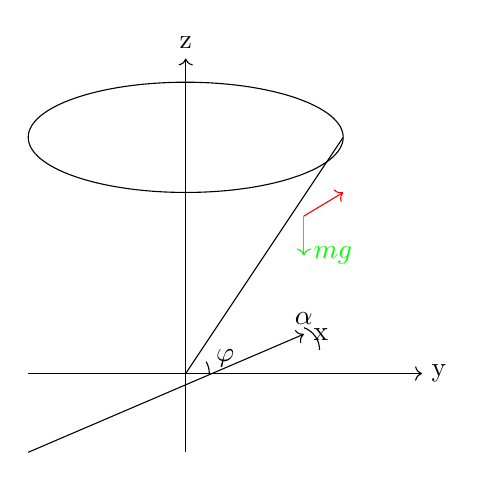
\begin{tikzpicture}
\draw[->] (-2,0) -- (3,0) node[right] {y};
\draw[->] (0,-1) -- (0,4) node[above] {z};
\draw[->] (-2,-1) -- (1.5,0.5) node[right] {x};
\draw (0,0) -- (2,3);
\draw (0,3) ellipse (2cm and 0.7cm);
\draw[dashed] (0,0) -- (2,0);
\draw (0.3,0) arc (0:30:0.3);
\node at (0.5,0.2) {$\varphi$};
\draw (1.7,0.3) arc (0:70:0.3);
\node at (1.5,0.7) {$\alpha$};
\draw[red,->] (1.5,2) -- (2,2.3);
\draw[green,->] (1.5,2) -- (1.5,1.5) node[right] {$mg$};
\end{tikzpicture}
\end{center}

Ein punktförmiges Teilchen der Masse m rollt auf der Innenseite eines Kreiskegels mit Öffnungswinkel $\alpha$ unter dem Einfluss eines konstanten Gravitationsfelds $\vec{g}$ in z-Richtung. Benutze Zylinderkoordinaten: $S,\varphi,z$.

Eine holonome ZB: $\tan \alpha = \frac{S}{z} \Leftrightarrow S-z\tan\alpha = 0$.

1. Schritt: 2 unabhängige generalisierte Koordinaten: $S,\varphi$

Zusammenhang mit kartesischen Koordinaten:
\[
\begin{pmatrix} 
x \\ y \\ z
\end{pmatrix} = 
\begin{pmatrix}
S \cos\varphi \\ S \sin\varphi \\ S \cot\alpha
\end{pmatrix}
\]

2. Schritt: Newtonsche Bewegungsgleichung in Kartesischen Koordinaten:

\[
m\begin{pmatrix}
\ddot{x} \\ \ddot{y} \\ \ddot{z}
\end{pmatrix} = 
\begin{pmatrix}
0 \\ 0 \\ -mg
\end{pmatrix} + 
\begin{pmatrix}
Z_x \\ Z_y \\ Z_z
\end{pmatrix}
\]
\begin{flushright}
Zwangskräfte
\end{flushright}


3. Schritt: Durch Berechnung zweier unabhängiger generalisierter Koordinaten

aus: $x = S\cos\varphi$
\[\begin{aligned}
\Rightarrow \dot{x} &= \dot{S}\cos\varphi - S\sin\varphi\dot{\varphi} \\
\Rightarrow \ddot{x} &= \ddot{S}\cos\varphi - \dot{S}\sin\varphi\dot{\varphi} - \dot{S}\sin\varphi\dot{\varphi} - S\cos\varphi\dot{\varphi}^2 - S\sin\varphi\ddot{\varphi} \\
&= \ddot{S}\cos\varphi - 2\dot{S}\dot{\varphi}\sin\varphi - S\dot{\varphi}^2\cos\varphi - S\ddot{\varphi}\sin\varphi
\end{aligned}\]

und analog für $y$, $z$ $\Rightarrow$

\begin{equation}
m(\ddot{S}\cos\varphi - 2\dot{S}\dot{\varphi}\sin\varphi - S\dot{\varphi}^2\cos\varphi - S\ddot{\varphi}\sin\varphi) = Z_x \tag{1}
\end{equation}

\begin{equation}
m(\ddot{S}\sin\varphi + 2\dot{S}\dot{\varphi}\cos\varphi - S\dot{\varphi}^2\sin\varphi + S\ddot{\varphi}\cos\varphi) = Z_y \tag{2}
\end{equation}

\begin{equation}
m(\ddot{S}\cot\alpha + g) = Z_z \tag{3}
\end{equation}

3 Gleichungen für 5 Unbekannte $S(t), \varphi(t), Z_x, Z_y, Z_z$.

3. Schritt: geometrische Überlegung: 

Zwangskraft $\vec{Z}$ steht immer senkrecht zur Kegelwand:


Von oben: 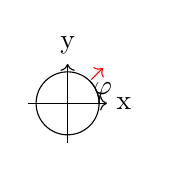
\begin{tikzpicture}[scale=0.5]
\draw[->] (-1,0) -- (1,0) node[right] {x};
\draw[->] (0,-1) -- (0,1) node[above] {y};
\draw (0,0) circle (0.8);
\draw[red,->] (0.6,0.6) -- (0.9,0.9);
\draw (0.8,0) arc (0:45:0.8);
\node at (0.9,0.3) {$\varphi$};
\end{tikzpicture}

\[\Rightarrow \begin{pmatrix} Z_x \\ Z_y \end{pmatrix} = -\sqrt{Z_x^2+Z_y^2}\begin{pmatrix} \cos\varphi \\ \sin\varphi \end{pmatrix} \tag{4}\]

Von der Seite: 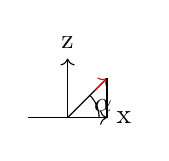
\begin{tikzpicture}[scale=0.5]
\draw[->] (-1,0) -- (1,0) node[right] {x};
\draw[->] (0,0) -- (0,1.5) node[above] {z};
\draw (0,0) -- (1,1);
\draw[red,->] (0.7,0.7) -- (1,1);
\draw (1,0) -- (1,1);
\draw (0.8,0) arc (0:45:0.8);
\node at (0.9,0.3) {$\alpha$};
\end{tikzpicture}
\[\Rightarrow 0 = \vec{Z} \cdot \begin{pmatrix} x \\ y \\ z \end{pmatrix} = Z_x\cos\varphi + Z_y\sin\varphi+Z_z\cot\alpha S \rightarrow Z_z = \sqrt{Z_x^2+Z_y^2}\tan\alpha\]

Damit ergeben sich aus (4) die beiden linearen Gleichungen:
\[Z_y \cos\varphi = Z_x \sin\varphi \tag{5}\]
\[Z_z \cos\varphi = -Z_x \tan\alpha \tag{6}\]

Strategie: Durch (5) und (6) nun auf (1) bis (3) zwei Gleichungen heraussuchen die nur die unabhängigen $S$ und $\varphi$ enthalten:

\[(1) * \sin\varphi - (2) * \cos\varphi \Rightarrow  2\dot{S}\dot{\varphi} + S\ddot{\varphi} = 0 \tag{7}\]

\[(1) * \tan\alpha + (3) * \cos\varphi \Rightarrow  (\tan\alpha + \cot\alpha)\ddot{S} - S\dot{\varphi}^2\tan\alpha + g = 0 \tag{8}\]

Gleichungen (7) und (8) enthalten nur die unabhängigen generalisierten Koordinaten $S$ und $\varphi$ - die ZK sind eliminiert. Wenn wir die Lösung dieser Gleichungen bestimmt haben, können wir die ZK durch Einsetzen in (1) bis (3) berechnen.

Nachteil des obigen Verfahrens:

Zunächst müssen die ZK in den Rechnungen mitgeführt werden und durch Untersuchung der Geometrie mühsam analysiert werden - letztendlich tauchen die ZK aber in den Bewegungsgleichungen der unabhängigen generalisierten Koordinaten nicht mehr auf.

Frage: Kann man die n Bewegungsgleichungen für die unabhängigen generalisierten Koordinaten auch direkt, d.h. ohne Betrachtung der ZK, aufstellen?

Antwort: Ja! D'Alembert, Lagrange!


\pagebreak

\subsubsection{Das d'Alembert Prinzip}

Darunter versteht man die folgende, mit der Erfahrung übereinstimmende Aussage über die Natur von Zwangkräften (ZK):

Gegeben sei ein System von N Massen $m_i$ auf die ZK $\vec{Z}_i$ wirken. Dann verschwindet die Summe der von den $\vec{Z}_i$ verrichteten ``virtuellen'' Zwangsarbeit:

\[
\delta W = \sum_{i=1}^N \vec{Z}_i \cdot \delta\vec{r}_i = 0.
\]

Die sogenannte ``virtuelle Verrückung'' $\delta\vec{r}_i$ des i-ten Teilchens ist dabei eine Verrückung des Teilchens mit den folgenden 3 Eigenschaften:
\begin{itemize}
\item sie ist infinitesimal
\item sie ist kompatibel mit den ZK
\item sie ist zeitlos ($\delta t=0$), d.h. unmittelbar schnell: die ZB sind während der virtuellen Verrückung als ruhend anzusehen.
\end{itemize}

\textbf{Anmerkungen:}

1) Wegen der 3. Eigenschaft gibt es bei Holonomen (d.h. zeitlosen) ZB einen Unterschied zwischen virtuellen Verrückungen $\delta\vec{r}_i$ und wirklichen Verrückungen $d\vec{r}_i$ die man durch Lösung der Bewegungsgleichungen mit ZB erhält.

\textbf{Beispiel:} Perle auf beschleunigtem Draht.

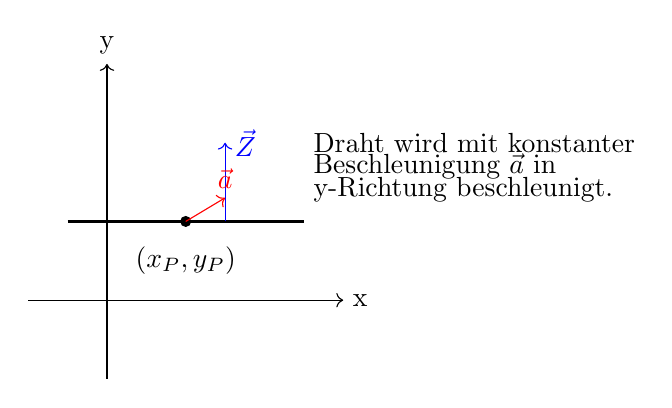
\begin{tikzpicture}
\draw[->] (-1,0) -- (3,0) node[right] {x};
\draw[->] (0,-1) -- (0,3) node[above] {y};
\draw[thick] (-0.5,1) -- (2.5,1);
\fill (1,1) circle (2pt);
\node at (1,0.5) {$(x_P,y_P)$};
\draw[blue,->] (1.5,1) -- (1.5,2) node[right] {$\vec{Z}$};
\draw[red,->] (1,1) -- (1.5,1.3) node[above] {$\vec{a}$};
\node[right] at (2.5,2) {Draht wird mit konstanter};
\node[right] at (2.5,1.7) {Beschleunigung $\vec{a}$ in};
\node[right] at (2.5,1.4) {y-Richtung beschleunigt.};
\end{tikzpicture}

$\Rightarrow$ holonome, rheonomische ZB: $y_P - \frac{1}{2}at^2 = 0$

\[
\Rightarrow \; \delta \vec{F} \text{ ist parallel zur } x\text{-Achse:} \quad \vec{Z} \cdot \delta \vec{F} = 0
\]
\[
d \vec{F} \text{ hat Komponente in } y\text{-Richtung:} \quad \vec{Z} \cdot d \vec{F} \neq 0
\]

d.h.: bei zeitabhängigen ZB ist die virtuelle Zwangsarbeit Null, nicht aber die reale Arbeit $\vec{Z} \cdot d\vec{r}$ der ZK.

2) Das d'Alembert-Prinzip ist eine Erfahrungstatsache, die nicht aus den Newtonschen Gesetzen hergeleitet werden kann. Es beruht auf der Erfahrung, dass Zwangsflächen, Achsen, Stangen, Fäden u.s.w. ein System nicht beschleunigen oder aufschaukeln, d.h. keine Zwangsarbeit leisten, es sei denn, sie werden durch Motore bewegt. Dann liegen aber rheonomische ZB vor, die reale aber keine virtuelle Zwangsarbeit leisten, wie im obigen Beispiel.

Aus den Newtonschen Bewegungsgleichungen für ein N-Teilchen-System mit ZK:

\[m_i \ddot{\vec{r}}_i = \vec{F}_i + \vec{Z}_i, \quad i=1,...,N\]

folgt: \[\sum_{i=1}^N (m_i \ddot{\vec{r}}_i-\vec{F}_i) \cdot \delta \vec{r}_i = \sum_{i=1}^N \vec{Z}_i \cdot \delta \vec{r}_i\]

und da die virtuelle Zwangsarbeit verschwindet $\Rightarrow$

\[\sum_{i=1}^N (m_i \ddot{\vec{r}}_i-\vec{F}_i) \cdot \delta \vec{r}_i = 0 \quad \text{(d'Alembert-Gleichung)}\]

Bei k holonomen ZB können daraus die Bewegungsgleichungen für die n unabhängigen generalisierten Koordinaten hergeleitet werden:
Drücken wir die Ortsvektoren durch die unabhängigen generalisierten Koordinaten aus (siehe S. 37):

\[\vec{r}_i = \vec{r}_i(q_1,...,q_n,t), \quad i=1,...,N\]

\[\Rightarrow \delta\vec{r}_i = \sum_{j=1}^n \frac{\partial\vec{r}_i}{\partial q_j}\delta q_j\]

So folgt aus der d'Alembert-Gleichung:

\[\sum_{j=1}^n \left[\sum_{i=1}^N (m_i\ddot{\vec{r}}_i-\vec{F}_i)\cdot\frac{\partial\vec{r}_i}{\partial q_j}\right]\delta q_j = 0\]

Da die $q_j$, $j=1,...,n$ aber alle unabhängig sind, muss jeder einzelne Term in der Klammer verschwinden $\Rightarrow$

\[\sum_{i=1}^N (m_i\ddot{\vec{r}}_i-\vec{F}_i)\cdot\frac{\partial\vec{r}_i}{\partial q_j} = 0, \quad j=1,...,n\]

Das sind n Gleichungen für die n unabhängigen generalisierten Koordinaten; die ZK kommen in diesen Bewegungsgleichungen nicht vor!



\textbf{Beispiel:} Teilchen auf Kreiskegel (siehe S. 37-39).

d'Alembert-Gleichung: $(m\ddot{\vec{r}}-m\vec{g})\cdot\delta\vec{r}=0$

\[\Leftrightarrow \ddot{x}\delta x + \ddot{y}\delta y + (\ddot{z}+g)\delta z = 0\]

ZB: $z = S\cot\alpha$

unabhängige generalisierte Koordinaten: $S,\varphi$ (Zylinderkoordinaten)

Zunächst müssen wir $\delta x, \delta y, \delta z$ durch die Variationen $\delta S, \delta\varphi$ der unabhängigen generalisierten Koordinaten ausdrücken:
Umrechnung von $\delta x, \delta y, \delta z$ auf $\delta S$ und $\delta \varphi$:
\[\begin{pmatrix} x \\ y \\ z \end{pmatrix} = \begin{pmatrix} S\cos\varphi \\ S\sin\varphi \\ S\cot\alpha \end{pmatrix} \Rightarrow \begin{pmatrix} \delta x \\ \delta y \\ \delta z \end{pmatrix} = \begin{pmatrix} \delta S\cos\varphi - S\sin\varphi\delta\varphi \\ \delta S\sin\varphi + S\cos\varphi\delta\varphi \\ \delta S\cot\alpha \end{pmatrix}\]

Jetzt müssen wir die kartesischen Komponenten der Beschleunigung durch die unabhängigen generalisierten Koordinaten ausdrücken; das haben wir bereits in Kapitel 2.2 (S.38) getan:

\[\begin{pmatrix} \ddot{x} \\ \ddot{y} \\ \ddot{z} \end{pmatrix} = \begin{pmatrix} \ddot{S}\cos\varphi - 2\dot{S}\dot{\varphi}\sin\varphi - S\dot{\varphi}^2\cos\varphi - S\ddot{\varphi}\sin\varphi \\ \ddot{S}\sin\varphi + 2\dot{S}\dot{\varphi}\cos\varphi - S\dot{\varphi}^2\sin\varphi + S\ddot{\varphi}\cos\varphi \\ \ddot{S}\cot\alpha \end{pmatrix}\]

Einsetzen in d'Alembert-Gleichung ergibt:
\[\begin{aligned}
0 &= \ddot{x}\delta x + \ddot{y}\delta y + (\ddot{z}+g)\delta z \\
&= \ddot{x}(\delta S\cos\varphi - S\sin\varphi\delta\varphi) + \ddot{y}(\delta S\sin\varphi + S\cos\varphi\delta\varphi) + (\ddot{z}+g)\delta S\cot\alpha \\
&= [\ddot{x}\cos\varphi + \ddot{y}\sin\varphi + (\ddot{z}+g)\cot\alpha]\delta S + [-\ddot{x}\sin\varphi + \ddot{y}\cos\varphi]S\delta\varphi \\
&= [(\tan\alpha + \cot\alpha)\ddot{S} - S\dot{\varphi}^2\tan\alpha + g]\delta S\cot\alpha + [2\dot{S}\dot{\varphi} + S\ddot{\varphi}]S\delta\varphi
\end{aligned}\]

\[\Rightarrow \boxed{
\begin{aligned}
2\dot{S}\dot{\varphi} + S\ddot{\varphi} &= 0 \\
(\tan\alpha + \cot\alpha)\ddot{S} - S\dot{\varphi}^2\tan\alpha + g &= 0
\end{aligned}
}\]
(siehe Gl.(7) und Gl.(8) auf S.39).

Diese Gleichungen haben wir in Kapitel 2.2 durch Eliminieren der ZK von den Newtonschen Bewegungsgleichungen erhalten. Der Vorteil der d'Alembert-Methode ist, dass wir die ZK nie explizit berechnen müssen.




Rezept: Bewegungsgleichungen für unabhängige generalisierte Koordinaten aus der d'Alembert Gleichung:

\begin{enumerate}
\item Schreibe d'Alembert-Gleichung in kartesischen Koordinaten hin.
\item Drücke kartesische Koordinaten durch unabhängige generalisierte Koordinaten aus.
\item Setze Koeffizienten der unabhängigen virtuellen Verrückungen gleich Null.
\end{enumerate}


\subsubsection*{Anmerkungen}

1) Das Gleichgewichtsprinzip der Mechanik

Dies ist ein Spezialfall der d'Alembert Gleichung $\sum_{i=1}^N(m_i\ddot{\vec{r}}_i-\vec{F}_i)\cdot\delta\vec{r}_i=0$:
Im Gleichgewicht wird nichts beschleunigt, so dass

\[\sum_{i=1}^N \vec{F}_i\cdot\delta\vec{r}_i = 0, \quad \text{d.h.: die virtuelle Arbeit}\]
\[\text{aller angreifenden Kräfte verschwindet im Gleichgewicht.}\]


2) Berechnung von ZK mit d'Alembert Gleichung:

Wir haben in Kapitel 2.1. gezeigt wie man ZK aus den Newtonschen Bewegungsgleichungen berechnen kann. Man kann die Zwangkräfte aber auch indirekt aus der d'Alembert Gleichung herleiten, obwohl sie dort nicht explizit auftreten. Dazu betrachtet man ein alternatives System, in dem diejenige ZK die man berechnen will formal als eingeprägte Kraft
behandelt wird. Die entsprechende ZB ist dann aufgehoben und man hat einen Freiheitsgrad mehr. Somit liefert die d'Alembert-Gleichung eine sechste Bedingung aus der die gesuchte eingeprägte Kraft bestimmt werden kann.



\textbf{Beispiel:} Leiter an Wand im Gleichgewicht:

\begin{center}
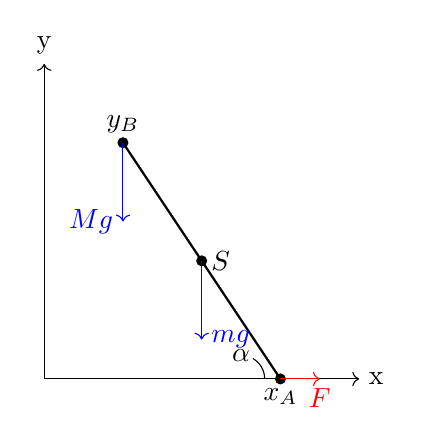
\begin{tikzpicture}
\draw[->] (0,0) -- (4,0) node[right] {x};
\draw[->] (0,0) -- (0,4) node[above] {y};
\draw[thick] (3,0) -- (1,3);
\fill (3,0) circle (2pt) node[below] {$x_A$};
\fill (1,3) circle (2pt) node[above] {$y_B$};
\fill (2,1.5) circle (2pt) node[right] {$S$};
\draw[blue,->] (2,1.5) -- (2,0.5) node[right] {$mg$};
\draw[blue,->] (1,3) -- (1,2) node[left] {$Mg$};
\draw[red,->] (3,0) -- (3.5,0) node[below] {$F$};
\draw (2.8,0) arc (0:60:0.3);
\node at (2.5,0.3) {$\alpha$};
\end{tikzpicture}
\end{center}

Leiter: Masse $M$, Länge $L$\\
Mensch: Masse $m$, Länge $\ell$\\
Eingeprägte Kräfte: $M\vec{g}$, $m\vec{g}$\\
ZK: Spannkraft $\vec{F}$ des Seils.\\
Frage: Wie groß ist $F$?

Behandle $\vec{F}$ als eingeprägte Kraft, der zusätzliche Freiheitsgrad ist die Position $\vec{r}_A$ des Auflagepunktes.

Gleichgewichtsprinzip: $M\vec{g} \cdot \delta\vec{r}_S + m\vec{g} \cdot \delta\vec{r}_B + \vec{F} \cdot \delta\vec{r}_A = 0$
$\Leftrightarrow -Mg \delta y_S - mg \delta y_B - F\delta x_A = 0$

ZB: $x_B = (L-\ell)\cos\alpha \quad x_S = \frac{L}{2} \cos\alpha \quad
    y_B = \ell \sin\alpha \quad y_S = \frac{L}{2} \sin\alpha$

Wegen $x_A = L\cos\alpha$ können wir alle virtuellen Verrückungen durch die Variation des Neigungswinkels ausdrücken:

$$\delta x_A = -L\sin\alpha \delta\alpha \quad
\delta y_B = \ell \cos\alpha \delta\alpha \quad
\delta y_S = \frac{L}{2} \cos\alpha \delta\alpha$$

Einsetzen im Gleichgewichtsprinzip
\[\Rightarrow(-Mg\frac{L}{2}\cos\alpha - mg\ell\cos\alpha + FL\sin\alpha)\delta\alpha = 0\]

\[\Rightarrow F = g\cot\alpha\left(\frac{M}{2} + m\frac{\ell}{L}\right)\]



\pagebreak

\subsubsection{Richtung der Zwangskräfte}

Das d'Alembertprinzip ist letztendlich eine Konsequenz aus der Erfahrungstatsache, dass die ZK immer senkrecht auf den Flächen stehen auf denen die Bewegung stattfindet.

Um dies besser zu verstehen, betrachten wir zunächst einen Massenpunkt dessen Bewegung durch eine holonome ZB der Form $f(\vec{r},t)=0$ eingeschränkt wird. Dann gilt die folgende Erfahrungstatsache:

Die ZK $\vec{Z} = m\ddot{\vec{r}}-\vec{F}$ steht senkrecht auf der durch $f(\vec{r},t)=0$ definierten Fläche, i.e. 
$$\vec{Z}(\vec{r},\dot{\vec{r}},t)=\lambda(\vec{r},\dot{\vec{r}},t)\nabla_rf(\vec{r},t)$$
Dabei ist $\lambda(\vec{r},\dot{\vec{r}},t)$ eine geeignete skalare Funktion. (Zur Erinnerung: $\nabla_rf = \text{grad }f$ steht senkrecht auf der Fläche $f(\vec{r},t) = \text{konst}$, siehe Mechanik I, M.43, S.149)



\textbf{Beispiel:} Klotz auf schiefer Ebene:

[Hier würde ein TikZ-Diagramm der schiefen Ebene folgen]

ZB: $\text{tand} = \frac{Y}{X}$ i.e. $f(\vec{r},t) = Y - X\text{ tand} = 0$
$$\Rightarrow \nabla_rf = \frac{\partial f}{\partial x}\vec{e}_x + \frac{\partial f}{\partial y}\vec{e}_y = -\text{tand }\vec{e}_x+\vec{e}_y$$


\textbf{Verallgemeinerung:}

a) N Teilchen, k holonome ZB: $f_j(\vec{r}_1,\dots,\vec{r}_N,t)=0, j=1,\dots,k$ $\Rightarrow$ ZK auf Teilchen i ist von der Form
$$\vec{Z}_i = \sum_{j=1}^k \lambda_j(\vec{r}_1,\dots,\vec{r}_N,\dot{\vec{r}}_1,\dots,\dot{\vec{r}}_N,t)\nabla_{r_i}f_j(\vec{r}_1,\dots,\vec{r}_N,t)$$
Diesen Ausdruck können wir auch schreiben als:

$$\vec{Z}_i = \sum_{j=1}^k \lambda_j(\vec{r}_1,\vec{r}_N,\dot{\vec{r}}_1,\dots,\dot{\vec{r}}_N,t)\vec{a}_{ji}(\vec{r}_1,\dots,\vec{r}_N,t)$$
wobei 
$$\vec{a}_{ji}(\vec{r}_1,\dots,\vec{r}_N,t) = \nabla_{r_i}f_j(\vec{r}_1,\dots,\vec{r}_N,t)$$

Die Notation ist dabei konsistent mit der in Kapitel 2.1c) eingeführten Notation,
$$a_{ji} = \frac{\partial h_j(q_1\dots q_n,t)}{\partial q_i}$$
für holonome ZB $h_j(q_1\dots q_n,t)=0$.



b) Liegen die ZB nur in differenzieller Form vor (siehe S. 29):
\[\sum_{i=1}^N \vec{a}_{ji}\cdot d\vec{r}_i + a_{jt}dt = 0, j=1,\dots,k\]
so gilt analog für die ZK auf Teilchen i,
\[\vec{Z}_i = \sum_{j=1}^k \lambda_j\vec{a}_{ji}.\]
Wir ziehen nun dann aus obigen Annahmen über die Richtung der ZK das d'Alembert-Prinzip heraus:

Für holonome ZB 
$$f_j(\vec{r}_1\dots\vec{r}_N,t)=0 \Rightarrow 0 = \delta f_j = \sum_{i=1}^N \nabla_{r_i}f_j(\vec{r}_1\dots\vec{r}_N,t)\cdot\delta\vec{r}_i = \sum_{i=1}^N \vec{a}_{ji}\cdot\delta\vec{r}_i$$
Die Gleichung $\sum_{i=1}^N \vec{a}_{ji}\cdot\delta\vec{r}_i=0$ gilt aber auch für differenzielle ZB, da bei virtuellen Verrückungen $\delta t = 0$ gitl:
$$\sum_{i=1}^N \vec{Z}_i\cdot\delta\vec{r}_i = \sum_{i=1}^N \sum_{j=1}^k \lambda_j\vec{a}_{ji}\cdot\delta\vec{r}_i = \sum_{j=1}^k \lambda_j(\sum_{i=1}^N \vec{a}_{ji}\cdot\delta\vec{r}_i) = 0$$




\subsubsection{Zusammenfassung der wichtigsten Ergebnisse von Kapitel 2}

\begin{enumerate}
    \item \textbf{d'Alembert-Prinzip:}
    
    $$
    \sum_{i=1}^N \vec{Z}_i \cdot \delta\vec{r}_i = 0
    $$
    
    Die virtuelle Zwangsarbeit verschwindet.

    \item \textbf{d'Alembert-Gleichung:}
    
    $$
    \sum_{i=1}^N (m_i \ddot{\vec{r}}_i - \vec{F}_i) \cdot \delta\vec{r}_i = 0
    $$

    \item \textbf{Bewegungsgleichungen der unabhängigen generalisierten Koordinaten \( q_1, \dots, q_n \) bei \( k \) holonomen Zwangsbedingungen:}
    
    $$
    \sum_{i=1}^N (m_i \ddot{\vec{r}}_i - \vec{F}_i) \cdot \frac{\partial\vec{r}_i}{\partial q_j} = 0,
    \quad j = 1, \dots, n
    $$

    \item \textbf{Gleichgewichtsprinzip:}
    
    $$
    \sum_{i=1}^N \vec{F}_i \cdot \delta\vec{r}_i = 0
    $$

    Die virtuelle Zwangsarbeit der eingeprägten Kräfte verschwindet im Gleichgewicht.
\end{enumerate}




\pagebreak


\subsection{Die Lagrangegleichungen 2. Art}


\subsubsection{Herleitung von ``Lagrange 2" aus der d'Alembert-Gleichung}



\textbf{Ausgangspunkt:} d'Alembert-Gleichung $\sum_{i=1}^N (m_i\ddot{\vec{r}}_i-\vec{F}_i)\cdot\delta\vec{r}_i = 0$.

Drücke die Ortsvektoren $\vec{r}_i$, $i=1,..,N$ des N-Teilchen Systems durch $n \leq 3N$ generalisierte Koordinaten $q_1,..,q_n$ aus.
(später werden wir annehmen dass diese unabhängig sind).
$$\vec{r}_i = \vec{r}_i(q_1,..,q_n,t),\ i=1,..,N \Rightarrow \delta\vec{r}_i = \sum_{j=1}^n \frac{\partial\vec{r}_i}{\partial q_j}\delta q_j$$
Die virtuelle Arbeit der eingeprägten Kräfte kann somit in der folgenden Form geschrieben werden:
$$\sum_{i=1}^N \vec{F}_i\cdot\delta\vec{r}_i = \sum_{j=1}^n\left(\sum_{i=1}^N \vec{F}_i\cdot\frac{\partial\vec{r}_i}{\partial q_j}\right)\delta q_j = \sum_{j=1}^n K_j\delta q_j$$
wobei
$$K_j = \sum_{i=1}^N \vec{F}_i\cdot\frac{\partial\vec{r}_i}{\partial q_j}$$ 
``generalisierte Kräfte genannt werden."


Als nächstes formen wir den ersten Term in der d'Alembert Gleichung um:

\begin{align*}
\sum_{i=1}^N m_i\ddot{\vec{r}}_i \cdot \delta\vec{r}_i 
&= \sum_{j=1}^n \left( \sum_{i=1}^N m_i \ddot{\vec{r}}_i \cdot \frac{\partial \vec{r}_i}{\partial q_j} \right) \delta q_j \\
&= \sum_{j=1}^n \left[ \sum_{i=1}^N \frac{d}{dt} \left( m_i \dot{\vec{r}}_i \cdot \frac{\partial \vec{r}_i}{\partial q_j} \right)
    - m_i \dot{\vec{r}}_i \cdot \frac{d}{dt} \left( \frac{\partial \vec{r}_i}{\partial q_j} \right) \right] \delta q_j
\end{align*}
(wegen $\frac{d}{dt}(g) = \frac{d}{dt}(\frac{\partial g}{\partial t}) - \frac{\partial}{\partial t}\frac{dg}{dt}$).


Nebenrechnungen:

a) wegen 
$$\dot{\vec{r}}_i = \sum_{j=1}^n \frac{\partial\vec{r}_i}{\partial q_j} \dot{q}_j + \frac{\partial\vec{r}_i}{\partial t} \Rightarrow \frac{\partial\vec{r}_i}{\partial q_j} = \frac{\partial\vec{r}_i}{\partial q_j}$$
b) wegen 
$$\frac{\partial\vec{r}_i}{\partial q_j} = \sum_{k=1}^n \frac{\partial^2\vec{r}_i}{\partial q_j\partial q_k} \dot{q}_k + \frac{\partial^2\vec{r}_i}{\partial q_j\partial t}$$
und 
$$\frac{d}{dt} \frac{\partial\vec{r}_i}{\partial q_j} = \sum_{k=1}^n \frac{\partial^2\vec{r}_i}{\partial q_j\partial q_k} \dot{q}_k + \frac{\partial^2\vec{r}_i}{\partial t\partial q_j}$$
folgt mit der Vertauschbarkeit der zweiten Ableitungen,
$$\frac{d}{dt} \left(\frac{\partial\vec{r}_i}{\partial q_j}\right) = \frac{\partial \dot{\vec{r}}_i}{\partial q_j}$$ 
Den ersten (kinetischen Energie) Term der d'Alembert-Gleichung können wir damit wie folgt umformen,
\begin{align*}
\sum_{i=1}^N m_i\ddot{\vec{r}}_i \cdot \delta\vec{r}_i 
&= \sum_{j=1}^n \left[ \sum_{i=1}^N \frac{d}{dt} \left( m_i \dot{\vec{r}}_i \cdot \frac{\partial \vec{r}_i}{\partial q_j} \right)
  - m_i \dot{\vec{r}}_i \cdot \frac{d}{dt} \left( \frac{\partial \vec{r}_i}{\partial q_j} \right) \right] \delta q_j \\
&= \sum_{j=1}^n \left[ \frac{d}{dt} \left( \frac{\partial}{\partial \dot{q}_j} \sum_{i=1}^N \frac{1}{2} m_i \dot{\vec{r}}_i^2 \right)
  - \frac{\partial}{\partial q_j} \sum_{i=1}^N \frac{1}{2} m_i \dot{\vec{r}}_i^2 \right] \delta q_j \\
&= \sum_{j=1}^n \left[ \frac{d}{dt} \left( \frac{\partial T}{\partial \dot{q}_j} \right) - \frac{\partial T}{\partial q_j} \right] \delta q_j
\end{align*}
wobei $$T = \sum_{i=1}^N \frac{1}{2}m_i\dot{\vec{r}}_i^2$$ 
die kinetische Energie ist.

Insgesamt folgt somit aus der d'Alembert-Gleichung:
$$\sum_{j=1}^n \left[\frac{d}{dt} \frac{\partial T}{\partial \dot{q}_j} - \frac{\partial T}{\partial q_j} - K_j\right] \delta q_j = 0$$



Nun machen wir 2 wichtige Annahmen:
\begin{enumerate}[label=\textbf{\arabic*)}, left=0pt, align=left, itemsep=1.2em]

  \item Es gibt \( k \) holonome Zwangsbedingungen, sodass $n = N - k = 3N - k$ generalisierte Koordinaten \( q_j \) unabhängig sind.

  Damit gilt das \textbf{d'Alembert-Lagrange-Prinzip} in folgender Form:
  \begin{equation*}
  \frac{d}{dt} \frac{\partial T}{\partial \dot{q}_j} - \frac{\partial T}{\partial q_j} - K_j = 0, 
  \quad j = 1, \dotsc, n = 3N - k \tag{1}
  \end{equation*}

  \item Die Kräfte lassen sich aus einem Potential ableiten:

  \begin{itemize}
    \item[(a)] Bei \textbf{konservativen Kräften} gilt:
    \[
    \vec{F}_i = - \vec{\nabla}_{r_i} V(\vec{r}_1, \dotsc, \vec{r}_N, t), 
    \quad i = 1, \dotsc, N
    \]
    Daraus folgt für die generalisierten Kräfte:
    \[
    \begin{aligned}
    K_j &= \sum_{i=1}^N \vec{F}_i \cdot \frac{\partial \vec{r}_i}{\partial q_j}
    = -\sum_{i=1}^N (\vec{\nabla}_i V) \cdot \frac{\partial \vec{r}_i}{\partial q_j} \\
    &= -\frac{\partial V(q_1, \dotsc, q_n, t)}{\partial q_j}
    \end{aligned}
    \]
    wobei
    \[
    V(q_1, \dotsc, q_n, t) 
    = V(\vec{r}_1, \dotsc, \vec{r}_N, t)\big|_{\vec{r}_i = \vec{r}_i(q_1, \dotsc, q_n, t)}
    \]

    \item[(b)] Sind die Kräfte \textbf{geschwindigkeitsabhängig} (z.B. Lorentzkraft im elektromagnetischen Feld auf eine Ladung \( e \)), so nehmen wir an, dass es ein \textbf{generalisiertes Potential}
    \[
    V(q_1, \dotsc, q_n, \dot{q}_1, \dotsc, \dot{q}_n, t)
    \]
    gibt, sodass die generalisierten Kräfte in folgender Form geschrieben werden können:
    \begin{equation*}
    K_j = -\frac{\partial V}{\partial q_j} + \frac{d}{dt} \frac{\partial V}{\partial \dot{q}_j} \tag{2}
    \end{equation*}
  \end{itemize}

\end{enumerate}





Beispiel: 

Elektromagnetische Kraft auf Teilchen der Ladung $Q$ (Lorentz-Kraft, siehe Elektrodynamik)

Das generalisierte Potential für ein geladenes Teilchen im elektromagnetischen Feld lautet:
\[
V(\vec{r}, \dot{\vec{r}}) = Q \left( \phi(\vec{r}) - \frac{1}{c} \dot{\vec{r}} \cdot \vec{A}(\vec{r}) \right),
\]
mit zugehöriger Kraft:
\[
\vec{F} = Q \left( \vec{E} + \frac{1}{c} \dot{\vec{r}} \times \vec{B} \right),
\]
wobei die Felder durch
\[
\vec{E} = -\vec{\nabla} \phi - \frac{1}{c} \frac{\partial \vec{A}}{\partial t}, 
\quad 
\vec{B} = \vec{\nabla} \times \vec{A}
\]
gegeben sind.

\vspace{1em}

Setzt man das generalisierte Potential \( V \) gemäß Gleichung (2) in die verallgemeinerten Bewegungsgleichungen (1) ein, so erhält man:
\[
\frac{d}{dt} \frac{\partial T}{\partial \dot{q}_j} - \frac{\partial T}{\partial q_j} 
- \left( \frac{d}{dt} \frac{\partial V}{\partial \dot{q}_j} - \frac{\partial V}{\partial q_j} \right) = 0, 
\quad j = 1, \dotsc, n = 3N - k.
\]

Dies führt zur Lagrange-Gleichung 2. Art:
\begin{equation*}
\frac{d}{dt} \frac{\partial L}{\partial \dot{q}_j} - \frac{\partial L}{\partial q_j} = 0, 
\quad j = 1, \dotsc, n = 3N - k,
\end{equation*}
wobei die Lagrange-Funktion definiert ist durch
\[
L(q_1, \dotsc, q_n, \dot{q}_1, \dotsc, \dot{q}_n, t) = T - V.
\]



Aus der Herleitung ist klar, dass diese Gleichungen nur bei holonomen ZB und nur bei Kräften, die sich aus generalisierten Potentialen herleiten lassen, gültig sind. In diesem Fall kann man die Bewegungsgleichungen für die unabhängigen generalisierten Koordinaten nach dem folgenden einfachen Rezept aufstellen:

\begin{enumerate}[label=\textbf{\arabic*)}, itemsep=1.5em]

  \item \textbf{Lagrange-Funktion in Abhängigkeit der $M = 3N$ generalisierten Koordinaten:}

  Die Lagrange-Funktion ist definiert als
  \[
  L = T - V,
  \]
  wobei sowohl die kinetische Energie \( T \) als auch das Potential \( V \) zunächst in Abhängigkeit der $M$ generalisierten Koordinaten \( \{ r_1, \dotsc, r_M \} \) sowie ihrer Zeitableitungen geschrieben werden:
  \[
  L = L(r_1, \dotsc, r_M, \dot{r}_1, \dotsc, \dot{r}_M, t).
  \]

  \item \textbf{Reduktion durch holonome Zwangsbedingungen:}

  Es seien \( k \) holonome Zwangsbedingungen gegeben. Damit verbleiben
  \[
  n = M - k = 3N - k
  \]
  unabhängige generalisierte Koordinaten \( \{ q_1, \dotsc, q_n \} \). Die ursprünglichen Koordinaten \( \{ r_i \} \) lassen sich durch die \( q_j \) ausdrücken:
  \[
  r_i = r_i(q_1, \dotsc, q_n, t), \quad i = 1, \dotsc, M.
  \]

  \item \textbf{Lagrange-Funktion in reduzierter Form:}

  Durch Einsetzen dieser Ausdrücke in \( T \) und \( V \) erhält man die reduzierte Lagrange-Funktion
  \[
  L(q_1, \dotsc, q_n, \dot{q}_1, \dotsc, \dot{q}_n, t),
  \]
  die nun ausschließlich von den unabhängigen Koordinaten \( q_j \), deren Zeitableitungen \( \dot{q}_j \) und der Zeit abhängt.

  \item \textbf{Lagrange-Gleichungen 2. Art:}

  Die Bewegungsgleichungen für die unabhängigen generalisierten Koordinaten ergeben sich aus dem Prinzip der stationären Wirkung und lauten:
  \[
  \frac{d}{dt} \frac{\partial L}{\partial \dot{q}_j} - \frac{\partial L}{\partial q_j} = 0,
  \quad j = 1, \dotsc, n.
  \]

\end{enumerate}




\subsubsection{Beispiel: Teilchen auf Kreiskegel (siehe S.33)}

\begin{center}
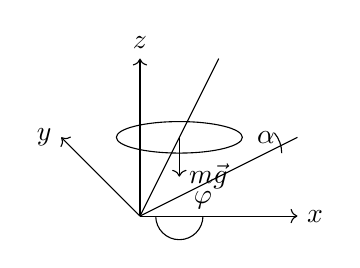
\begin{tikzpicture}
\draw[->] (0,0) -- (2,0) node[right] {$x$};
\draw[->] (0,0) -- (0,2) node[above] {$z$};
\draw[->] (0,0) -- (-1,1) node[left] {$y$};
\draw (0,0) -- (2,1);
\draw (0,0) -- (1,2);
\draw (0.5,1) ellipse (0.8cm and 0.2cm);
\draw[->] (0.5,1) -- (0.5,0.5) node[right] {$m\vec{g}$};
\draw (0.2,0) arc (180:360:0.3);
\node at (0.8,0.2) {$\varphi$};
\draw (1.8,0.8) arc (0:40:0.4);
\node at (1.6,1) {$\alpha$};
\end{tikzpicture}
\end{center}

holonome ZB: $\rho-z\tan\alpha=0$

Die Bewegungsgleichungen für die unabhängigen generalisierten Koordinaten haben wir bereits in Kapitel 2.2 (S.33) im Rahmen der Newtonschen Mechanik aufgestellt. Mit dem Lagrange-Formalismus ist der Zugang systematischer:
\begin{enumerate}
    \item Die Lagrange-Funktion lautet zunächst:
    \[
    L = T - V = \frac{m}{2} \left( \dot{s}^2 + s^2 \dot{\varphi}^2 \right) - mgz
    \]

    \item Durch die Zwangsbedingung ergibt sich:
    \[
    z = s \cos\alpha
    \]

    \item Einsetzen ergibt:
    \[
    L(s, \dot{s}, \varphi, \dot{\varphi}) 
    = \frac{m}{2} \left( (1 + \cos^2\alpha)\dot{s}^2 + s^2 \dot{\varphi}^2 \right) - mgs\cos\alpha
    \]

    \item Die Lagrange-Gleichungen für \( s \) und \( \varphi \) lauten:

    \[
    \frac{d}{dt} \left( \frac{\partial L}{\partial \dot{s}} \right) - \frac{\partial L}{\partial s}
    = m\left[(1 + \cos^2\alpha) \ddot{s} - s \dot{\varphi}^2 + g \cos\alpha\right] = 0
    \]

    \[
    \frac{d}{dt} \left( \frac{\partial L}{\partial \dot{\varphi}} \right) - \frac{\partial L}{\partial \varphi}
    = m s^2 \left( 2 \dot{s} \dot{\varphi} + s \ddot{\varphi} \right) = 0
    \]

\end{enumerate}

Diese beiden Gleichungen stimmen exakt mit den auf Seite 33 im Rahmen der Newtonschen Mechanik gefundenen Bewegungsgleichungen überein.


\pagebreak


\subsubsection{Forminvarianz der Lagrangegleichungen}

Wir zeigen nun dass die Lagrangegleichungen bei beliebigen Punkttransformationen zu neuen generalisierten Koordinaten,
$$q_j' = q_j'(q_1,..,q_n,t), \quad j=1,..,n$$
ihre Form behalten, d.h. forminvariant sind.
Ausgangspunkt: $L(q_1,..,q_n,\dot{q}_1,..,\dot{q}_n,t), \quad n=3N-k=N-k$
$$\dfrac{d}{dt}\dfrac{\partial L}{\partial \dot{q}_j} - \dfrac{\partial L}{\partial q_j} = 0, \quad j=1,..,n$$
Notation: $q=\{q_1,..,q_n\}, \quad \dot{q}=\{\dot{q}_1,..,\dot{q}_n\}, \quad L=L(q,\dot{q},t)$
Punkttransformation: $q'=q'(q,t), \quad$ inverse $q=q(q',t)$

Wir erhalten die Lagrangefunktion $L'(q',\dot{q}',t)$ der neuen Koordinaten und Geschwindigkeiten durch Einsetzen der inversen Transformation in die alte Lagrangefunktion, d.h.
$$L'(q',\dot{q}',t) = L(q(q',t),\dot{q}(q',\dot{q}',t),t)$$
D.h. die Lagrangefunktion ändert zwar ihre Form, nicht aber ihren Wert - das ist das Transformationsverhalten eines Skalars.

Wir zeigen nun dass
$$\dfrac{d}{dt}\dfrac{\partial L'}{\partial \dot{q}_j'} - \dfrac{\partial L'}{\partial q_j'} = 0, \quad j=1,..,n$$
D.h. die Lagrangegleichungen der neuen Lagrangefunktion, ausgedrückt durch die neuen Koordinaten, haben die selbe Form wie die ursprünglichen Lagrangegleichungen.

Beweis:

Betrachte eine Koordinatentransformation
\[
q_i = q_i(q_1', \dotsc, q_n', t),
\]
unter der sich die Lagrange-Funktion transformiert zu:
\[
L' = L(q(q',t), \dot{q}(q', \dot{q}', t), t).
\]
Wir berechnen die Ableitungen:
\begin{align*}
\frac{\partial L'}{\partial q_j'} 
&= \frac{\partial}{\partial q_j'} L(q(q',t), \dot{q}(q', \dot{q}', t), t) \\
&= \sum_{i=1}^n \left( 
    \frac{\partial L}{\partial q_i} \frac{\partial q_i}{\partial q_j'} 
  + \frac{\partial L}{\partial \dot{q}_i} \frac{\partial \dot{q}_i}{\partial q_j'} 
\right), \\[1ex]
\frac{\partial L'}{\partial \dot{q}_j'} 
&= \frac{\partial}{\partial \dot{q}_j'} L(q(q',t), \dot{q}(q', \dot{q}', t), t) 
= \sum_{i=1}^n \frac{\partial L}{\partial \dot{q}_i} \frac{\partial \dot{q}_i}{\partial \dot{q}_j'}.
\end{align*}
Wie auf S.54 gezeigt, gilt:
\begin{align*}
\text{a)}\quad &\frac{\partial \dot{q}_i}{\partial \dot{q}_j'} = \frac{\partial q_i}{\partial q_j'}, \\
\text{b)}\quad &\frac{d}{dt} \left( \frac{\partial q_i}{\partial q_j'} \right) = \frac{\partial \dot{q}_i}{\partial q_j'}.
\end{align*}
\textbf{Begründung:}  
Da \( q_i = q_i(q', t) \), folgt:
\[
\dot{q}_i = \sum_k \frac{\partial q_i}{\partial q_k'} \dot{q}_k' + \frac{\partial q_i}{\partial t}
\Rightarrow \text{a)} \quad \frac{\partial \dot{q}_i}{\partial \dot{q}_j'} = \frac{\partial q_i}{\partial q_j'}.
\]
Ableitung nach der Zeit ergibt:
\[
\frac{d}{dt} \left( \frac{\partial q_i}{\partial q_j'} \right)
= \sum_k \frac{\partial^2 q_i}{\partial q_k' \partial q_j'} \dot{q}_k' + \frac{\partial^2 q_i}{\partial t \partial q_j'}
= \frac{\partial \dot{q}_i}{\partial q_j'}, \quad \text{(b) wegen Vertauschung der Ableitungen}.
\]
Damit folgt:
\begin{align*}
\frac{\partial L'}{\partial \dot{q}_j'} 
&= \sum_{i=1}^n \frac{\partial L}{\partial \dot{q}_i} \frac{\partial q_i}{\partial q_j'}, \\
\Rightarrow \frac{d}{dt} \left( \frac{\partial L'}{\partial \dot{q}_j'} \right)
&= \sum_{i=1}^n \left( 
  \frac{d}{dt} \left( \frac{\partial L}{\partial \dot{q}_i} \right) \frac{\partial q_i}{\partial q_j'} 
+ \frac{\partial L}{\partial \dot{q}_i} \frac{d}{dt} \left( \frac{\partial q_i}{\partial q_j'} \right) 
\right) \\
&= \sum_{i=1}^n \left( 
  \frac{d}{dt} \left( \frac{\partial L}{\partial \dot{q}_i} \right) \frac{\partial q_i}{\partial q_j'} 
+ \frac{\partial L}{\partial \dot{q}_i} \frac{\partial \dot{q}_i}{\partial q_j'}
\right).
\end{align*}
Ebenso:
\[
\frac{\partial L'}{\partial q_j'} 
= \sum_{i=1}^n \left( 
  \frac{\partial L}{\partial q_i} \frac{\partial q_i}{\partial q_j'} 
+ \frac{\partial L}{\partial \dot{q}_i} \frac{\partial \dot{q}_i}{\partial q_j'} 
\right).
\]
Subtraktion ergibt:
\begin{align*}
\frac{d}{dt} \left( \frac{\partial L'}{\partial \dot{q}_j'} \right) - \frac{\partial L'}{\partial q_j'}
&= \sum_{i=1}^n \left( 
  \frac{d}{dt} \left( \frac{\partial L}{\partial \dot{q}_i} \right) 
  - \frac{\partial L}{\partial q_i} \right) \frac{\partial q_i}{\partial q_j'}.
\end{align*}
Ist \( L \) eine Lösung der Lagrange-Gleichungen:
\[
\frac{d}{dt} \left( \frac{\partial L}{\partial \dot{q}_i} \right) - \frac{\partial L}{\partial q_i} = 0,
\]
so folgt:
\[
\frac{d}{dt} \left( \frac{\partial L'}{\partial \dot{q}_j'} \right) - \frac{\partial L'}{\partial q_j'} = 0.
\]
\textbf{Fazit:}  
Die Lagrange-Gleichungen sind \emph{forminvariant} unter regulären Koordinatentransformationen.

Wichtig: die Lagrangegleichungen behalten ihre Form auch in beschleunigten Bezugssystemen, also nicht-Inertialsystemen!




\textbf{Beispiel:} freies Teilchen in einer Dimension im beschleunigten Bezugssystem:

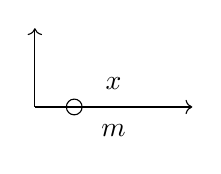
\begin{tikzpicture}
\draw[->] (0,0) -- (2,0);
\draw[->] (0,0) -- (0,1);
\node at (1,0.3) {$x$};
\node at (1,-0.3) {$m$};
\draw (0.5,0) circle (0.1);
\end{tikzpicture}

Lagrangefunktion im Inertialsystem:
$L(x,\dot{x},t) = T(\dot{x}) = \dfrac{1}{2}m\dot{x}^2$

$\Rightarrow \dfrac{d}{dt}\dfrac{\partial L}{\partial \dot{x}} - \dfrac{\partial L}{\partial x} = m\ddot{x} = 0$

Wir betrachten die Bewegung nun von einem beschleunigten Bezugssystem aus, das mit Beschleunigung $A(t)$ entlang der x-Achse beschleunigt wird:

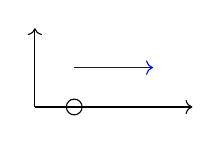
\begin{tikzpicture}
\draw[->] (0,0) -- (2,0);
\draw[->] (0,0) -- (0,1);
\draw[blue,->] (0.5,0.5) -- (1.5,0.5);
\draw (0.5,0) circle (0.1);
\end{tikzpicture}

Zusammenhang zwischen neuen und alten Koordinaten:
$x' = x - \int_0^t dt' V(t'), \quad A = \dfrac{dV}{dt}$

$\Rightarrow \dot{x}' = \dot{x} - V, \quad \dot{x} = \dot{x}' + V$

Die neue Lagrangefunktion erhält man durch Einsetzen der inversen Transformationsgleichung in die alte:

$L'(x',\dot{x}',t) = L(x(x',t),\dot{x}(x',\dot{x}',t),t) = \dfrac{m}{2}(\dot{x}' + V)^2$
$\Rightarrow \frac{d}{dt}\frac{\partial L'}{\partial \dot{x}'} - \frac{\partial L'}{\partial x'} = \frac{d}{dt}(m(\dot{x}'+V)) = m(\ddot{x}'+A) = 0$

$\Rightarrow m\ddot{x}' = -mA \uparrow$

\noindent Scheinkraft auf Grund der Transformation!

Die in beschleunigten Bezugssystemen auftretenden Scheinkräfte sind also automatisch in den Lagrangegleichungen enthalten!





\subsubsection{Freies Teilchen in einer Dimension im beschleunigten Bezugssystem}


\begin{center}
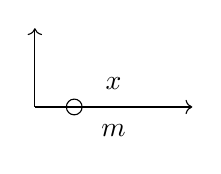
\begin{tikzpicture}
\draw[->] (0,0) -- (2,0);
\draw[->] (0,0) -- (0,1);
\node at (1,0.3) {$x$};
\node at (1,-0.3) {$m$};
\draw (0.5,0) circle (0.1);
\end{tikzpicture}
\end{center}

Die Lagrangefunktion im Inertialsystem lautet:
\[
L(x,\dot{x},t) = T(\dot{x}) = \frac{1}{2} m \dot{x}^2
\]
Die Lagrange-Gleichung ergibt:
\[
\frac{d}{dt} \frac{\partial L}{\partial \dot{x}} - \frac{\partial L}{\partial x} = m \ddot{x} = 0
\]
Wir betrachten nun ein Bezugssystem, das sich entlang der \( x \)-Achse mit zeitabhängiger Beschleunigung \( A(t) \) bewegt:

\begin{center}
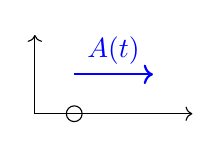
\begin{tikzpicture}
\draw[->] (0,0) -- (2,0);
\draw[->] (0,0) -- (0,1);
\draw[blue,->, thick] (0.5,0.5) -- (1.5,0.5);
\draw (0.5,0) circle (0.1);
\node[blue] at (1,0.8) {$A(t)$};
\end{tikzpicture}
\end{center}

Der Zusammenhang zwischen den Koordinaten ist:
\[
x' = x - \int_0^t V(t') \, dt', 
\quad \text{mit} \quad A(t) = \frac{dV}{dt}
\]
Daraus folgt für die Geschwindigkeiten:
\[
\dot{x}' = \dot{x} - V(t), 
\quad \Rightarrow \dot{x} = \dot{x}' + V(t)
\]
Einsetzen in die ursprüngliche Lagrangefunktion ergibt die transformierte Lagrangefunktion im beschleunigten System:
\[
L'(x', \dot{x}', t) = L(x(x', t), \dot{x}(x', \dot{x}', t), t) = \frac{m}{2}(\dot{x}' + V(t))^2
\]
Anwenden der Lagrange-Gleichung im beschleunigten System:
\[
\frac{d}{dt} \left( \frac{\partial L'}{\partial \dot{x}'} \right) - \frac{\partial L'}{\partial x'} 
= \frac{d}{dt} \left( m (\dot{x}' + V(t)) \right) = m (\ddot{x}' + A(t)) = 0
\]
Daraus folgt:
\[
m \ddot{x}' = -m A(t)
\]

\noindent\textbf{Interpretation:}  
Die Scheinkraft \( -mA(t) \) tritt ganz natürlich in der Lagrange-Gleichung auf – sie ist eine direkte Folge der Transformation in ein beschleunigtes Bezugssystem.  
\\[1ex]
\textit{Die in beschleunigten Bezugssystemen auftretenden Scheinkräfte sind also automatisch in den Lagrange-Gleichungen enthalten!}









\pagebreak



\subsection{Symmetrien, Invarianzen, Erhaltungsgrößen}

Die Lagrange'sche Mechanik macht die Zusammenhänge zwischen diesen Konzepten besonders transparent. Zunächst wollen wir aber präzisieren, was man darunter versteht.

\subsubsection{Begriffe}

a) \textbf{Symmetrien}

Ein physikalisches System heißt symmetrisch in Bezug auf eine gewisse Operation, wenn nach dem Ausführen dieser Operation kein Unterschied am System zu erkennen ist.

\textbf{Beispiel:} Kugel, symmetrisch bezüglich Drehung um Mittelpunkt.


\textbf{b) Invarianzen}

Ein System sei symmetrisch bezüglich einer Operation, die durch die Transformation $q_i \rightarrow q_i'$ der generalisierten Koordinaten beschrieben wird. Symmetrie manifestiert sich in der Invarianz der Lagrangefunktion:

Vor Transformation: $L(q,\dot{q},t)$. Bei allgemeinen Punkttransformationen $q = q'(q',t)$ transformiert sich $L$ wie ein Skalar (siehe S.55):
$$L'(q',\dot{q}',t) = L(q(q',t),\dot{q}(q',\dot{q}',t),t)$$
Liegt jedoch eine Invarianz vor, so ist die transformierte Lagrangefunktion dieselbe Funktion der neuen Koordinaten wie die ursprüngliche Lagrangefunktion, d.h.
$$L'(q',\dot{q}',t) = L(q\to q',\dot{q}\to\dot{q}',t)$$
Liegt also keine Symmetrie vor, so hat die transformierte Lagrangefunktion eine andere funktionale Abhängigkeit der neuen Koordinaten als die ursprüngliche Lagrangefunktion der alten; wir haben dies bereits im Beispiel auf S.57 gesehen: freies Teilchen: 
$$L(x,\dot{x},t) = \frac{m}{2}\dot{x}^2$$
Übergang zu beschleunigtem Bezugssystem: 
$$x' = x-\int_0^t dt' V(t') \Rightarrow L'(x',\dot{x}',t) = \frac{m}{2}(\dot{x}'+V)^2 \neq L(x\to x',\dot{x}\to\dot{x}',t)$$
Liegt jedoch eine Symmetrie vor, so können wir die neue Lagrangefunktion einfach durch Substitution der alten durch die neuen Koordinaten aus der alten Lagrangefunktion erhalten:




\textbf{Beispiel:} Teilchen im zylindersymmetrischen Potential:
$$L(\vec{r},\dot{\vec{r}}) = \frac{m}{2}(\dot{x}^2+\dot{y}^2+\dot{z}^2) - V(x^2+y^2,z)$$
Invarianz bezüglich Rotation um z-Achse: $\begin{pmatrix} X \\ Y \end{pmatrix} = \begin{pmatrix} \cos\alpha & -\sin\alpha \\ \sin\alpha & \cos\alpha \end{pmatrix} \begin{pmatrix} x' \\ y' \end{pmatrix}$
$$\Rightarrow L'(\vec{r}',\dot{\vec{r}}') = L(\vec{r},\dot{\vec{r}})$$




\textbf{c) Erhaltungsgrößen:}


Darunter verstehen wir Funktionen der Form $f(q_1,..,q_n,\dot{q}_1,..,\dot{q}_n,t)$ mit der Eigenschaft dass für alle Lösungen $q_i(t)$ der Bewegungsgleichungen
$$\frac{d}{dt}f(q_1,..,q_n,\dot{q}_1,..,\dot{q}_n,t) = 0$$




\subsection*{d) Kanonische Impulse (auch: generalisierte/konjugierte Impulse)}

Der zu einer generalisierten Koordinate $q_i$ gehörige kanonische Impuls ist definiert durch
\[p_i = \frac{\partial L}{\partial \dot{q_i}}\]
Damit lässt sich die Lagrangegleichung umschreiben:
\[\frac{d}{dt}\frac{\partial L}{\partial \dot{q_i}} - \frac{\partial L}{\partial q_i} = 0 \quad \Rightarrow \quad \dot{p_i} = \frac{\partial L}{\partial q_i} \quad \forall i \forall t\]




\textbf{Beispiel:} geladenes Teilchen im elektromagnetischen Feld (siehe S.62):
\[L(\vec{r},\dot{\vec{r}}) = \frac{m}{2}\dot{\vec{r}}^2 - V(\vec{r},\dot{\vec{r}}), \quad V(\vec{r},\dot{\vec{r}}) = Q(\phi - \frac{\dot{\vec{r}}}{c}\cdot\vec{A})\]

\[\Rightarrow \vec{p} = m\dot{\vec{r}} + \frac{Q}{c}\vec{A} \quad \text{: Kanonischer Impuls}\]
mit $m\dot{\vec{r}}$ als kinematischer Impuls. 

Für geschwindigkeitsabhängige Potentiale gilt im Allgemeinen:
Kanonischer Impuls $\neq$ Kinematischer Impuls.





\textbf{e) Zyklische Koordinaten}

Darunter versteht man alle generalisierten Koordinaten, die nicht explizit in der Lagrangefunktion auftreten (sondern höchstens über ihre zeitlichen Ableitungen \( \dot{q}_i \)).
\[
\Rightarrow \frac{\partial L}{\partial q_i} = 0 
\quad \text{für eine zyklische Koordinate } q_i
\]
Aus der Lagrange-Gleichung folgt:
\[
\frac{d}{dt} \left( \frac{\partial L}{\partial \dot{q}_i} \right) = \frac{\partial L}{\partial q_i} = 0
\quad \Rightarrow \quad \dot{p}_i = 0
\]
\[
\Rightarrow \quad p_i = \text{konstant}
\quad \text{(kanonischer Impuls von } q_i \text{ ist erhalten).}
\]

\noindent
\textbf{Fazit:}  
Zyklische Koordinaten führen direkt zu Erhaltungsgrößen. Dies ist ein Spezialfall des Noether-Theorems, wobei die Invarianz unter Verschiebung in \( q_i \) eine Impulserhaltung impliziert.



Bei der Lösung des Zweikörperproblems mit konservativen Zentralkräften (Siehe Kapitel 9, Mechanik I) haben wir gesehen, dass Erhaltungsgrößen sehr nützlich sind, weil
\begin{itemize}
\item sich damit die Bewegung qua Natur diskutieren läßt
\item sich damit die explizite Lösung der Bewegungsgleichungen vereinfachen läßt.
\end{itemize}

Es ist daher zur konkreten Lösung mechanischer Probleme zweckmäßig, die generalisierten Koordinaten so zu wählen, dass möglichst viele $q_j$ zyklisch sind.

\textbf{Beispiel:} Teilchen auf Kreiskegel (siehe S.69, S.71)

\[L(s,\dot{s},\varphi,\dot{\varphi}) = \frac{m}{2}\left((1+\cos^2\alpha)\dot{s}^2 + s^2\dot{\varphi}^2\right) - mgs\cos\alpha\]

hängt nicht von $\varphi$ ab ($\varphi$ ist zyklisch)

\[\Rightarrow p_\varphi = \frac{\partial L}{\partial \dot{\varphi}} = ms^2\dot{\varphi} \text{ ist erhalten (Drehimpuls um z-Achse)}\]

Da das System konservativ ist, ist auch die Energie E erhalten:

\[E = \frac{m}{2}\vec{v}^2 + mgz = \frac{m}{2}\left((1+\cos^2\alpha)\dot{s}^2 + \frac{\dot{\varphi}^2}{m^2s^2}\right) + mgs\cos\alpha\]

\[\Rightarrow E - \frac{p_\varphi^2}{2ms^2} - mgs\cos\alpha = \frac{m}{2}\dot{s}^2\frac{\sin^2\alpha+\cos^2\alpha}{\sin^2\alpha}\]

\[\Rightarrow \dot{s} = \pm\sin\alpha\sqrt{\frac{2}{m}\left(E - \frac{p_\varphi^2}{2ms^2} - mgs\cos\alpha\right)}\]

\[\Rightarrow t-t_0 = \pm\frac{1}{\sin\alpha}\int_{s_0}^s\frac{ds}{\sqrt{\frac{2}{m}\left(E - \frac{p_\varphi^2}{2ms^2} - mgs\cos\alpha\right)}}\]

Daraus kann man $t=t(s)$ berechnen. Auflösen nach $s=s(t)$ und Einsetzen in $\varphi(t)-\varphi(t_1)=\frac{p_\varphi}{m}\int_{t_0}^t\frac{dt}{s^2(t)}$ liefert auch den Winkel $\varphi(t)$.



\subsubsection{Der Noether-Theorem} 

(Emmy Noether, 1882-1935) Dies ist eine mathematische Formulierung des Zusammenhangs
\[
\text{Symmetrie} \Rightarrow \text{Invarianz} \Rightarrow \text{Erhaltungsgröße}
\]

\textbf{Ausgangspunkt:}\\
Koordinatentransformation, die stetig differenzierbar von einem kontinuierlichen Parameter $\alpha$ abhängt:

\[q_i \to q_i'(q_1,\ldots,q_n,t;\alpha), \quad i=1,\ldots,n = 3N-k\]

Die Transformation sei invertierbar, d.h. wir können auflösen:
\[q_i = q_i(q_1',\ldots,q_n',t;\alpha)\]

Ferner sei es für $\alpha=0$ die identische Transformation,
\[q_i'(q_1,\ldots,q_n,t;\alpha=0) = q_i\]

\textbf{Beispiele}
\begin{itemize}
\item Translation: $\vec{r} \to \vec{r}' = \vec{r} + \alpha\vec{a}$
\item Rotation:\\
Um z-Achse: $\begin{pmatrix} x \\ y \\ z \end{pmatrix} \to \begin{pmatrix} x' \\ y' \\ z' \end{pmatrix} = \begin{pmatrix} \cos\alpha & \sin\alpha & 0 \\ -\sin\alpha & \cos\alpha & 0 \\ 0 & 0 & 1 \end{pmatrix} \begin{pmatrix} x \\ y \\ z \end{pmatrix} = \begin{pmatrix} x\cos\alpha+y\sin\alpha \\ -x\sin\alpha+y\cos\alpha \\ z \end{pmatrix}$
\end{itemize}

Notation (siehe S.55): $q = q'(q,t;\alpha), \quad q = q(q',t;\alpha)$

Wir betrachten nun die transformierte Lagrangefunktion, die gemäß den allgemeinen Transformationsvorhalten auf S.54 gegeben ist durch
\[L'(q_i',\dot{q_i}',t;\alpha) = L(q(q_i',t;\alpha), \dot{q}(q',\dot{q}',t;\alpha), t)\]
Ableiten nach $\alpha$ bei konstantem $q'$ und $\dot{q}'$ ergibt:

\[\frac{\partial L'}{\partial \alpha} = \sum_{i=1}^n \left\{\frac{\partial L}{\partial q_i}\frac{\partial q_i(q',t;\alpha)}{\partial \alpha} + \frac{\partial L}{\partial \dot{q_i}}\frac{d}{dt}\left[\frac{\partial q_i(q',t;\alpha)}{\partial \alpha}\right]\right\}\]

\[= \sum_{i=1}^n \left\{\frac{d}{dt}\frac{\partial L}{\partial \dot{q_i}}\frac{\partial q_i}{\partial \alpha} + \frac{\partial L}{\partial \dot{q_i}}\frac{d}{dt}\frac{\partial q_i}{\partial \alpha}\right\}\]

\[= \frac{d}{dt}\left\{\sum_{i=1}^n \frac{\partial L}{\partial \dot{q_i}}\frac{\partial q_i(q',t;\alpha)}{\partial \alpha}\right\}\]

\[= \frac{d}{dt}\left\{\sum_{i=1}^n p_i\frac{\partial q_i}{\partial \alpha}\right\}\]

Natürlich gilt diese Gleichung auch wenn wir nach der Differentiation $\alpha=0$ setzen, d.h.

\[\left.\frac{\partial L'(q',\dot{q}',t;\alpha)}{\partial \alpha}\right|_{\alpha=0} = \frac{d}{dt}\sum_{i=1}^n p_i\left.\frac{\partial q_i(q',t;\alpha)}{\partial \alpha}\right|_{\alpha=0}\]

Wir nehmen nun an, dass die Transformation $q'=q'(q,t;\alpha)$ eine Symmetrietransformation ist, d.h. die Lagrangefunktion invariant lässt, so dass (siehe S. 60):

\[L'(q',\dot{q}',t;\alpha) = L(q',\dot{q}',t) \Rightarrow \frac{\partial L'}{\partial \alpha} = 0\]



\textbf{Noether Theorem:}

Ist die Lagrangefunktion unter der kontinuierlichen, stetig differenzierbaren Koordinatentransformation $q\to q'(q,t;\alpha)$ invariant, so ist die folgende Funktion $I(q,\dot{q},t)$ eine Erhaltungsgröße:

\[I(q,\dot{q},t) = \sum_{i=1}^n p_i\left.\frac{\partial q_i(q',t;\alpha)}{\partial \alpha}\right|_{\alpha=0}\]




\subsubsection{Beispiele}

1) 

Der auf S.61 hergeleitete Erhaltungssatz für kanonische Impulse von zyklischen Koordinaten ist ein Spezialfall des Noether-Theorems: Da L bei definitivem von zyklischen Koordinaten nicht abhängt, ist in diesem Fall L invariant unter einer Translation 
$$q_i \rightarrow q_i - \alpha \Rightarrow \left.\frac{\partial q_i}{\partial \alpha}\right|_{\alpha=0} = \left.\frac{\partial (q_i+\alpha)}{\partial \alpha}\right|_{\alpha=0} = 1 \quad \Rightarrow\quad I(q,\dot{q},t) = p_i = \frac{\partial L}{\partial \dot{q_i}}$$



2) 

Teilchen im zylindersymmetrischen Potential (siehe S.60):
\[L = \frac{m}{2}(\dot{x}^2 + \dot{y}^2 + \dot{z}^2) - V(\sqrt{x^2+y^2},z)\]
invariant bezüglich Rotation um z-Achse:
\[\begin{pmatrix} x \\ y \end{pmatrix} = \begin{pmatrix} \cos\alpha & -\sin\alpha \\ \sin\alpha & \cos\alpha \end{pmatrix} \begin{pmatrix} x' \\ y' \end{pmatrix}, L'(\vec{r}',\dot{\vec{r}}',t) = L(\vec{r},\dot{\vec{r}},t)\]
Damit ergibt sich die Erhaltungsgröße:
\[I = p_x \left.\frac{\partial x(x',y',\alpha)}{\partial \alpha}\right|_{\alpha=0} + p_y \left.\frac{\partial y(x',y',\alpha)}{\partial \alpha}\right|_{\alpha=0}\]
\[= m\dot{x}(-x'\sin\alpha-y'\cos\alpha) + m\dot{y}(x'\cos\alpha-y'\sin\alpha)\Big|_{\alpha=0}\]
\[= m(x\dot{y}-y\dot{x}) = m(\vec{r}\times\dot{\vec{r}})_z = L_z\]

Schneller geht's in Zylinderkoordinaten, da $\varphi$ dann zyklisch ist:
\[L = \frac{m}{2}(\dot{\rho}^2 + \rho^2\dot{\varphi}^2 + \dot{z}^2) - V(\rho,z), \text{ invariant unter } \varphi \rightarrow \varphi-\alpha\]
Wir erhatlen
$$I = p_\varphi \left.\frac{\partial}{\partial\alpha}(\varphi'+\alpha)\right|_{\alpha=0} = p_\varphi = \frac{\partial L}{\partial\dot{\varphi}} = m\rho^2\dot{\varphi} = L_z$$




\subsubsection{Allgemeine Form des Noether-Theorems}

Manchmal kommt es vor, dass gewisse Koordinaten-transformationen $q \to q'(q_i,t;\alpha)$ die Lagrangefunktion zwar nicht invariant lassen, aber nur eine zusätzliche totale Zeitableitung erzeugen:
\[L'(q',\dot{q}',t;\alpha) = L(q',\dot{q}',t) + \frac{d}{dt}F(q',t;\alpha)\]
wobei $F(q',t;\alpha)$ eine beliebige Funktion der Koordinaten ist.

Man nennt in diesem Fall die Lagrangefunktion ``symmetrisch'' unter der Transformation, und $q \to q'(q_i,t;\alpha)$ Symmetrietransformation. Die totale Zeitableitung ändert jedoch die Bewegungsgleichungen nicht, denn es gilt allgemein (``Eichinvarianz der Bewegungsgleichungen'').

Für beliebige Funktionen $F(q,t)$ der Koordinaten und der Zeit haben die beiden Lagrangefunktionen $L(q,\dot{q},t)$ und 
\[\tilde{L}(q,\dot{q},t) = L(q,\dot{q},t) + \frac{d}{dt}F(q,t)\] dieselben Bewegungsgleichungen.




\textbf{Beweis:}

\[\frac{d}{dt}\frac{\partial \tilde{L}}{\partial \dot{q}} - \frac{\partial \tilde{L}}{\partial q} = \frac{d}{dt}\frac{\partial L}{\partial \dot{q}} - \frac{\partial L}{\partial q} + \frac{d}{dt}\underbrace{\left(\frac{\partial}{\partial \dot{q}}\frac{dF}{dt}\right)}_{=0} - \frac{\partial}{\partial q}\frac{dF}{dt}\]

Das die Terme mit $\frac{dF}{dt}$ verschwinden sieht man so:
\[\frac{d}{dt}F(q,t) = \frac{\partial F}{\partial q}\dot{q} + \frac{\partial F}{\partial t}\]
\[\Rightarrow \frac{d}{dt}\frac{\partial}{\partial q}\frac{dF}{dt} = \frac{d}{dt}\frac{\partial F}{\partial q} = \frac{\partial^2 F}{\partial q^2}\dot{q} + \frac{\partial^2 F}{\partial t\partial q}\]

andererseits: \[\frac{\partial}{\partial q}\frac{dF}{dt} = \frac{\partial^2 F}{\partial q^2}\dot{q} + \frac{\partial^2 F}{\partial t\partial q}\]
(Reihenfolge vertauscht)

\[\Rightarrow \frac{d}{dt}\left(\frac{\partial}{\partial \dot{q}}\frac{dF}{dt}\right) - \frac{\partial}{\partial q}\frac{dF}{dt} = 0\]
Aus dem modifizierten Transformationsverhalten:
\[L'(q',\dot{q}',t;\alpha) = L(q',\dot{q}',t) + \frac{d}{dt}F(q',t;\alpha)\]

folgt
\[\left.\frac{\partial L'(q',\dot{q}',t;\alpha)}{\partial \alpha}\right|_{\alpha=0} = \frac{d}{dt}\left.\frac{\partial F(q',t;\alpha)}{\partial \alpha}\right|_{\alpha=0}\]

und nach denselben Rechnungen wie auf S.64 ergibt sich die Erhaltungsgröße:
\[I(q,\dot{q},t) = \sum_{i=1}^n p_i\left.\frac{\partial q_i}{\partial \alpha}\right|_{\alpha=0} - \left.\frac{\partial F}{\partial \alpha}\right|_{\alpha=0}\]





\subsubsection{Beispiel} 

freier Fall im homogenen Schwerefeld:
\[L(x,\dot{x}) = \frac{m}{2}\dot{x}^2 - mgx\]

Eigentliche Galileitransformationen sind Symmetrietransformationen:
\[x \to x' = x + \alpha t, \quad \alpha = \text{``boost-Geschwindigkeit''}\]
denn:
\begin{align*}
L'(x',\dot{x}',t;\alpha) &= \frac{m}{2}(\dot{x}'-\alpha)^2 - mg(x'-\alpha t) \\
&= \frac{m}{2}\dot{x}'^2 - mgx' + \alpha m\left(gt-\dot{x}'\right) + \frac{m}{2}\alpha^2 \\
&= L(x',\dot{x}') + \frac{d}{dt}\left[\alpha m\left(\frac{g}{2}t^2-x'\right) + \frac{m}{2}\alpha^2t\right]
\end{align*}
mit 
$$F(x',t;\alpha)=\alpha m\left(\frac{g}{2}t^2-x'\right) + \frac{m}{2}\alpha^2t$$
Wir erhalten die Erhaltungsgröße:
\begin{align*}
I(x,\dot{x},t) &= \frac{\partial L}{\partial \dot{x}}\left.\frac{\partial x'(x,t;\alpha)}{\partial \alpha}\right|_{\alpha=0} - \left.\frac{\partial F}{\partial \alpha}\right|_{\alpha=0} \\
&= m\dot{x}(-t) - m\left(\frac{g}{2}t^2-x\right) \\
&= m\left(x-\dot{x}t - \frac{g}{2}t^2\right)
\end{align*}
folgt aus Lösung der Bewegungsgleichung!




\subsubsection{Energieerhaltung}


\textbf{Symmetrie:} Homogenität der Zeit\\

$\Rightarrow$ \textbf{Invarianz:} Für $t_0$ beliebig
$$L(q,\dot{q},t+t_0) = L(q,\dot{q},t)$$ 
d.h. 
$$\frac{\partial L}{\partial t} = 0$$
oder: $L(q,\dot{q})$ hängt nicht explizit von Zeit ab.


Bei unserer Herleitung des Noether-Theorems haben wir uns auf Transformationen der Form $q_i \to q_i'(q,t;\alpha)$ beschränkt, die Zeittranslationen nicht mit einschließen. Daher können wir das Noether-Theorem nicht benutzen, um die mit der Homogenität der Zeit zusammenhängende Erhaltungsgröße zu berechnen.


Wir leiten daher $L(q,\dot{q})$ direkt nach t ab:
\[\frac{d}{dt}L = \sum_{i=1}^n \left(\frac{\partial L}{\partial q_i}\dot{q_i} + \frac{\partial L}{\partial \dot{q_i}}\ddot{q_i}\right)\]
\[= \sum_{i=1}^n \left(\frac{d}{dt}\frac{\partial L}{\partial \dot{q_i}}\dot{q_i} + \frac{\partial L}{\partial \dot{q_i}}\ddot{q_i}\right) = \frac{d}{dt}\left(\sum_{i=1}^n \frac{\partial L}{\partial \dot{q_i}}\dot{q_i}\right) = \frac{d}{dt}\left(\sum_{i=1}^n p_i\dot{q_i}\right)\]
\[\Leftrightarrow \frac{d}{dt}\left(\sum_{i=1}^n p_i\dot{q_i} - L\right) = 0\]
Wenn wir die Gleichungen $p_i = \frac{\partial L}{\partial \dot{q_i}}$ nach $\dot{q_i} = \dot{q_i}(q,p)$ auflösen und die Funktion
\[H = \sum_{i=1}^n p_i\dot{q_i} - L(q_i,\dot{q_i})\]
als Funktion der generalisierten Koordinaten und der entsprechenden Impulse $p_i$ auffassen, so wird H die Hamiltonfunktion des Systems genannt. Es gilt somit:


Hängt die Lagrangefunktion $L(q,\dot{q})$ nicht explizit von der Zeit ab, so ist die Hamiltonfunktion $H(q,p)$ erhalten.

Zur physikalischen Interpretation von H betrachten wir den Spezialfall:
\begin{enumerate}
\item Konservative Kräfte
\item holonome, skleronome Zwangsbedingungen
\item zeitunabhängige Transformationsgleichungen zu generalisierten Koord. (unbewegtes Bezugssystem)
\end{enumerate}
$$1) \Rightarrow \frac{\partial L}{\partial \dot{q}_i} = \frac{\partial T}{\partial \dot{q}_i} = p_i$$
$$2),3) \Rightarrow \vec{r}_i = \vec{r}_i(q_1,..,q_n)$$
Die kinetische Energie kann dann wie folgt geschrieben werden:
\[T = \sum_{i=1}^N \frac{m_i}{2}\dot{\vec{r}}_i^2 = \sum_{i=1}^N \sum_{\alpha,\beta=1}^n \frac{m_i}{2}\left(\frac{\partial \vec{r}_i}{\partial q_\alpha}\dot{q}_\alpha\right)\cdot\left(\frac{\partial \vec{r}_i}{\partial q_\beta}\dot{q}_\beta\right)\]
\[= \sum_{\alpha,\beta=1}^n q_{\alpha\beta}\dot{q}_\alpha\dot{q}_\beta, \text{ wobei } q_{\alpha\beta} = q_{\beta\alpha} = \sum_{i=1}^N \frac{m_i}{2}\frac{\partial \vec{r}_i}{\partial q_\alpha}\cdot\frac{\partial \vec{r}_i}{\partial q_\beta}\]

$$\Rightarrow p_i = \frac{\partial T}{\partial \dot{q}_i} = 2\sum_{\alpha=1}^n q_{i\alpha}\dot{q}_\alpha$$
$$\Rightarrow \sum_{i=1}^n p_i\dot{q}_i = 2\sum_{i,\alpha=1}^n q_{i\alpha}\dot{q}_i\dot{q}_\alpha = 2T$$
$$\Rightarrow H = \sum_{i=1}^n p_i\dot{q}_i - L = 2T-(T-V) = T+V = E$$
d.h.: Für konservative Kräfte und holonome, skleronome ZB sowie zeitunabhängige Transformationsgleichungen zu generalisierten Koordinaten ist die Hamiltonfunktion gleich der Gesamtenergie.




\subsubsection{Zusammenfassung Kapitel 4:}

1) \textbf{Noether-Theorem:}

Kontinuierliche Schar von Koordinatentransformationen:
\[q_i \to q_i' = q_i'(q_1,..,q_n,t;\alpha), \quad i=1,..,n=3N-R.\]

Falls Lagrangefunktion bis auf totale Zeitableitung invariant ist,
\[L'(q',\dot{q}',t;\alpha) = L(q',\dot{q}',t) + \frac{dF(q',t;\alpha)}{dt}\]

ist die folgende Größe erhalten:
\[I(q,\dot{q},t) = \sum_{i=1}^n \frac{\partial L}{\partial \dot{q_i}} \left.\frac{\partial q_i(q',t;\alpha)}{\partial \alpha}\right|_{\alpha=0} - \left.\frac{\partial F(q',t;\alpha)}{\partial \alpha}\right|_{\alpha=0}\]

2) \textbf{Zyklische Koordinaten} (Spezialfall von Noether-Theorem)
\[\frac{\partial L}{\partial q_i} = 0 \quad \Rightarrow \quad p_i = \text{Konst.}\]

3) \textbf{Zusammenhang Symmetrie, Invarianz, Erhaltungsgrößen:}

\begin{tabular}{|l|l|l|}
\hline
Symmetrie & Invarianz & Erhaltungsgröße \\
\hline
Homogenität des & Translations- & Impuls \\
Raumes & invarianz & \\
\hline
Isotropie des & Rotationsinvarianz & Drehimpuls \\
Raumes & & \\
\hline
Homogenität der & Invarianz unter & Energie \\
Zeit & Zeittranslation & \\
\hline
\end{tabular}



\pagebreak


\subsection{Die Lagrangegleichungen 1. Art}


Die im Kapitel 3 hergeleiteten Lagrangegleichungen 2. Art,
\[\frac{d}{dt}\frac{\partial L}{\partial \dot{q}_i} - \frac{\partial L}{\partial q_i} = 0,\]
gelten nur bei holonomen ZB. Ferner lassen sich die ZK
\[\vec{Z}_i = m_i\ddot{\vec{r}}_i-\vec{F}_i\] erst berechnen, wenn man die Bewegungsgleichungen gelöst hat. Die in diesem Kapitel diskutierten Lagrangegleichungen 1. Art gelten auch für beliebige differenzielle ZB. Ferner eignet sich ``Lagrange 1'' besonders gut zur expliziten Berechnung der ZK.

\subsubsection{Herleitung von ``Lagrange 1'' aus d'Alembert}

Ausgangspunkt (wie bei Lagrange 2): d'Alembert-Gleichung:
\[\sum_{i=1}^N (m_i\ddot{\vec{r}}_i-\vec{F}_i)\cdot\delta\vec{r}_i = 0\]
Wie bei Lagrange 2 erhalten wir daraus (siehe S. 51)
\[\sum_{j=1}^n \left[\frac{d}{dt}\frac{\partial T}{\partial \dot{q}_j} - \frac{\partial T}{\partial q_j} - K_j\right]\delta q_j = 0\]
mit \[K_j = \sum_{i=1}^N \vec{F}_i\cdot\frac{\partial \vec{r}_i}{\partial q_j} \text{ : geneigte Kräfte.}\]
Wie auf S. 52 nehmen wir an, dass sich die $K_j$ aus einem generalisierten Potential $V(q_1,..,q_n,\dot{q}_1,..,\dot{q}_n,t)$ ableiten lassen,
\[K_j = -\frac{\partial V}{\partial q_j} + \frac{d}{dt}\frac{\partial V}{\partial \dot{q}_j},\]
so dass mit $L = T-V$ gilt:
\[\sum_{j=1}^n \left(\frac{d}{dt}\frac{\partial L}{\partial \dot{q}_j} - \frac{\partial L}{\partial q_j}\right)\delta q_j = 0 \tag{1}\]
Bei Lagrange 2 hatten wir an dieser Stelle $n=M-h=3N-k =$ Anzahl der unabhängigen generalisierten Koordinaten gesetzt. Dann muss jeder einzelne Term in (1) verschwinden. Nun jedoch setzen wir $n=M=3N =$ maximale Anzahl der generalisierten Koordinaten. Ferner nehmen wir an, dass die Bewegung des Systems durch $k$ differenzielle ZB der Form (siehe S. 25)
\[\sum_{i=1}^M a_{ji} \dot{q}_i + a_{j0} dt = 0, \quad j=1,..,k\]
eingeschränkt ist. Für virtuelle Verrückungen ($dt=0$) gilt dann
\[\sum_{i=1}^M a_{ji} \delta q_i = 0, \quad j=1,..,k \tag{2}\]
Wegen der ZB sind nicht alle $q_i$ unabhängig, so dass aus (1) mit $n=M$ nicht gefolgert werden kann, dass jeder einzelne Term verschwindet. Aus (1) und (2) folgt jedoch:
\[\sum_{i=1}^M \left[\frac{d}{dt}\frac{\partial L}{\partial \dot{q}_i} - \frac{\partial L}{\partial q_i} - \sum_{j=1}^k \lambda_j a_{ji}\right]\delta q_i = 0,\]
wobei die $\lambda_j$, $j=1,..,k$, vorerst noch unbekannte Faktoren sind (die sogenannten ``Lagrangeschen Multiplikatoren'').

Wegen (2) sind von den $M=3N$ Verrückungen $\delta q_i$ $k$ voneinander abhängig. Wir betrachten die ersten $M-k$ Verrückungen $\delta q_1,..,\delta q_{M-k}$ als unabhängig und spalten die obige Summe auf:
\[\sum_{i=1}^{M-k} \left[\frac{d}{dt}\frac{\partial L}{\partial \dot{q}_i} - \frac{\partial L}{\partial q_i} - \sum_{j=1}^k \lambda_j a_{ji}\right]\delta q_i\]
\[+ \sum_{i=M-k+1}^M \left[\frac{d}{dt}\frac{\partial L}{\partial \dot{q}_i} - \frac{\partial L}{\partial q_i} - \sum_{j=1}^k \lambda_j a_{ji}\right]\delta q_i = 0\]
Wähle nun die $\lambda_j$ so, dass jede der k Klammern verschwindet!

Da aber die ersten M-k Verrückungen $\delta q_i$ unabhängig sind, muss auch jede der Klammern in 1. Term verschwinden.

$\Rightarrow$ Lagrangegleichungen 1. Art:
\[\frac{d}{dt}\frac{\partial L}{\partial \dot{q}_i} - \frac{\partial L}{\partial q_i} = \sum_{j=1}^k \lambda_j a_{ji}, \quad i=1,..,M=3N \quad \text{(3) Bewegung}\]



Zur Interpretation des Terms auf der rechten Seite stellen wir uns vor, dass alle ZB aufgehoben wurden und durch ihr Effekt durch zusätzliche äußere Kräfte $\vec{F}_i^Z$ kompensiert wird. Dann gilt nach Lagrange 2 (siehe S. 50, S. 52):
\[\frac{d}{dt}\frac{\partial L}{\partial \dot{q}_i} - \frac{\partial L}{\partial q_i} = K_i^Z, \quad K_i^Z = \sum_{j=1}^N \vec{F}_j^Z \cdot \frac{\partial \vec{r}_j}{\partial q_i}\]
\[\Rightarrow \sum_{j=1}^k \lambda_j a_{ji} = \sum_{j=1}^N \vec{Z}_j \cdot \frac{\partial \vec{r}_j}{\partial q_i} = Z_{q_i}\]
ist die generalisierte Zwangskraft auf Freiheitsgrad i.

Sind die Lagrangemultiplikatoren $\lambda_j$ bekannt, so können wir aber die ZK berechnen.




\subsubsection{Gebrauchsanweisung von ``Lagrange 1''}

\begin{enumerate}[label=\textbf{\arabic*)}, itemsep=1.5em]

\item \textbf{Wähle \( M = 3N \) geeignete generalisierte Koordinaten}  
\[
q_1, q_2, \dotsc, q_M
\]
zur Beschreibung eines Systems aus \( N \) Massenpunkten im dreidimensionalen Raum.

\item \textbf{Schreibe die Zwangsbedingungen (ZB) in differentieller Form:}
\[
\sum_{i=1}^M a_{ji}(q, t) \, dq_i + a_{j0}(q, t)\, dt = 0, \quad j = 1, \dotsc, k
\]

Im Fall von \textbf{holonomen} Zwangsbedingungen der Form
\[
h_j(q_1, \dotsc, q_M, t) = 0,
\]
gilt:
\[
a_{ji} = \frac{\partial h_j}{\partial q_i}, 
\quad
a_{j0} = \frac{\partial h_j}{\partial t}
\]

\item \textbf{Drücke die Lagrange-Funktion \( L = T - V \)} als Funktion der \( 2M \) Variablen aus:
\[
L = L(q_1, \dotsc, q_M, \dot{q}_1, \dotsc, \dot{q}_M, t)
\]

\item \textbf{Stelle die Lagrange-Gleichungen 1. Art auf:}
\[
\frac{d}{dt} \left( \frac{\partial L}{\partial \dot{q}_i} \right) 
- \frac{\partial L}{\partial q_i} 
= \sum_{j=1}^k \lambda_j a_{ji}, 
\quad i = 1, \dotsc, M
\]

Die \(\lambda_j\) sind \textbf{Lagrange-Multiplikatoren}, welche die Wirkung der Zwangskräfte erfassen.

\item \textbf{Löse das Gleichungssystem:}

\vspace{0.5em}
\noindent
\begin{tabular}{@{}ll}
\textbf{Unbekannte:} 
& \( \underbrace{q_1, \dotsc, q_M}_{M} 
\quad + \quad 
\underbrace{\lambda_1, \dotsc, \lambda_k}_{k} 
= M + k \) \\[1ex]

\textbf{Gleichungen:} 
& \( M \) Lagrange-Gleichungen der 1. Art \\[0.5ex]
& \( + \; k \) Zwangsbedingungen (z.B. \( h_j(q, t) = 0 \)) \\[1ex]

\textbf{Gesamt:} 
& \( M + k \) Gleichungen für \( M + k \) Unbekannte
\end{tabular}

\vspace{1.5em}
\noindent
\textbf{Hinweis:}  
In vielen Fällen ist es zweckmäßig, die \( k \) Zwangsbedingungen zuerst zu verwenden, um die Lagrange-Multiplikatoren \( \lambda_j \) zu eliminieren. Dadurch kann das Gleichungssystem reduziert und effizienter gelöst werden.

\end{enumerate}



\subsubsection{Beispiele zu Lagrange 1}

Beispiel: Teilchen auf Kreiskegel


Dieses Beispiel wurde bereits in Kapitel 2.2 (S.37) mit Newton und in Kapitel 3.1 (S.54) mit Lagrange 2. Art behandelt.  
Nun folgt die Behandlung mit \textbf{Lagrange 1. Art}, bei der auch die \textbf{Zwangskräfte explizit} berechnet werden können.

\begin{enumerate}[label=\textbf{\arabic*)}, itemsep=1.5em]

\item \textbf{Systembeschreibung:}  
Ein Teilchen der Masse \( m \) bewegt sich auf einem Kreiskegel.  
Anzahl der Massenpunkte: \( N = 1 \)  
\[
\Rightarrow M = 3 \quad \text{(Dimension = 3)}
\]  
Generalisierte Koordinaten:
\[
q_1 = S, \quad q_2 = \varphi, \quad q_3 = z
\]

\item \textbf{Zwangsbedingung (ZB):}
\[
h(S, \varphi, z) = S - z \tan\alpha = 0 \quad \Rightarrow \quad k = 1
\]
Differenzielle Form:
\[
dS - \tan\alpha \, dz = 0
\]
Daraus folgt der Normalenvektor des Zwangs:
\[
\sigma_S = 1, \quad \sigma_z = -\tan\alpha
\]

\item \textbf{Lagrangefunktion:}
\[
L = T - V = \frac{m}{2} \left( \dot{S}^2 + S^2 \dot{\varphi}^2 + \dot{z}^2 \right) - mgz
\]

\item \textbf{Lagrange-Gleichungen 1. Art:}

\begin{align*}
\text{(1)}\quad & m(\ddot{S} - S \dot{\varphi}^2) = \lambda \sigma_S = \lambda \\[0.5em]
\text{(2)}\quad & m(2 \dot{S} \dot{\varphi} + S \ddot{\varphi}) = 0 \\[0.5em]
\text{(3)}\quad & m(\ddot{z} + g) = \lambda \sigma_z = -\lambda \tan\alpha
\end{align*}

Dies sind 3 Gleichungen für 4 Unbekannte: \( S(t), \varphi(t), z(t), \lambda(t) \).  
Die \textbf{4. Gleichung} ist die Zwangsbedingung:
\[
S = z \tan\alpha
\]

\item \textbf{Generalisierte Zwangskräfte:}

\begin{align*}
Z_S &= \vec{Z} \cdot \frac{\partial \vec{r}}{\partial S} = \lambda \\[0.5em]
Z_z &= \vec{Z} \cdot \frac{\partial \vec{r}}{\partial z} = -\lambda \tan\alpha \quad \text{(vgl. S.38)}
\end{align*}

\item \textbf{Reduktion mit Hilfe der Zwangsbedingung:}

Multipliziere Gleichung (1) mit \( \tan\alpha \) und addiere Gleichung (3):

\begin{align*}
&\tan\alpha \cdot m(\ddot{S} - S \dot{\varphi}^2) + m(\ddot{z} + g) = 0 \\
\Rightarrow \; & (\tan\alpha + \cot\alpha) \ddot{S} - S \dot{\varphi}^2 \tan\alpha = g
\end{align*}

(vgl. S.39 und S.54)

\item \textbf{Zwangskraft \(\lambda\) explizit (ohne Lösung der Bewegungsgleichungen):}

Nutze die ZB \( S = z \tan\alpha \) und eliminiere \( \ddot{z} \) aus (1) und (3):

\[
\begin{cases}
m(\tan\alpha \ddot{z} - S \dot{\varphi}^2) = \lambda \\
m(\tan\alpha \ddot{z} + \tan\alpha g) = -\lambda \tan\alpha
\end{cases}
\]

Addition ergibt:

\[
m(-S \dot{\varphi}^2 - g \tan\alpha) = \lambda (1 + \tan^2\alpha)
\]

\[
\Rightarrow \lambda = -\frac{m}{1 + \tan^2\alpha} \left( g \tan\alpha + S \dot{\varphi}^2 \right)
\]

Mit \( \rho^2 := m S^2 \dot{\varphi}^2 \) (Zentrifugalanteil) folgt auch:
\[
\lambda = -m \cdot \frac{g \tan\alpha + \frac{\rho^2}{m S^2}}{1 + \tan^2\alpha}
\]

\end{enumerate}






Einkantwagen

Ein schräg gestellter Einkantwagen wird angestoßen und bewegt sich danach frei auf einer ebenen Fläche.

\vspace{1em}
\textbf{Gegeben:}
\begin{align*}
m &= \text{Gesamtmasse des Wagens} \\
I_s &= \text{Trägheitsmoment um die } z\text{-Achse durch den Schwerpunkt } S
\end{align*}

\textbf{Generalisierte Koordinaten:}
\[
x_A, \quad y_A \quad \text{(Position des Achsenmittelpunkts)}, 
\quad \alpha \quad \text{(Winkel der Fahrtrichtung zur } x\text{-Achse)}
\]

\textbf{Zwangsbedingung (nicht-holonome ZB)}

Die momentane Fahrtrichtung ist stets senkrecht zur Achse:

\[
\frac{dy_A}{dx_A} = \tan\alpha 
\quad \Leftrightarrow \quad
\dot{x}_A \sin\alpha - \dot{y}_A \cos\alpha = 0
\]

\noindent
In differentieller Form:

\[
\sin\alpha \, dx_A - \cos\alpha \, dy_A = 0
\quad \Rightarrow \quad
a_{x_A} = \sin\alpha, \quad a_{y_A} = -\cos\alpha
\]

\textbf{Kinetische Energie}

Nach dem \textbf{König-Theorem} (siehe Mechanik I):

\[
T = \frac{m}{2} (\dot{x}_S^2 + \dot{y}_S^2) + \frac{I_s}{2} \dot{\alpha}^2
\]

mit den Beziehungen:

\begin{align*}
x_S &= x_A + l \cos\alpha 
&\Rightarrow \quad \dot{x}_S &= \dot{x}_A - l \dot{\alpha} \sin\alpha \\
y_S &= y_A + l \sin\alpha 
&\Rightarrow \quad \dot{y}_S &= \dot{y}_A + l \dot{\alpha} \cos\alpha
\end{align*}

\textbf{Lagrange-Funktion \( L = T - V \)}

Da \( V = 0 \), folgt:

\begin{align*}
L(x_A, y_A, \alpha, \dot{x}_A, \dot{y}_A, \dot{\alpha}) 
&= \frac{m}{2} \left[ (\dot{x}_A - l \dot{\alpha} \sin\alpha)^2 + (\dot{y}_A + l \dot{\alpha} \cos\alpha)^2 \right] + \frac{I_s}{2} \dot{\alpha}^2 \\[1ex]
&= \frac{m}{2} (\dot{x}_A^2 + \dot{y}_A^2) 
+ \frac{I_A}{2} \dot{\alpha}^2 
+ m l \dot{\alpha} ( \dot{y}_A \cos\alpha - \dot{x}_A \sin\alpha )
\end{align*}

mit dem \textbf{Trägheitsmoment um Punkt A} nach dem Satz von Steiner:

\[
I_A = I_s + m l^2
\]

\textbf{Zwangsbedingung in differentieller Form}
\[
\sin\alpha \cdot dx_A - \cos\alpha \cdot dy_A = 0
\quad \Rightarrow \quad
q_{x_A} = \sin\alpha, \quad q_{y_A} = -\cos\alpha
\]
Diese nicht-holonome, lineare Zwangsbedingung ist der Ausgangspunkt für die Anwendung der Lagrange-Gleichungen 1. Art mit Lagrange-Multiplikator \( \lambda \):
\[
\frac{d}{dt} \frac{\partial L}{\partial \dot{q}_i} - \frac{\partial L}{\partial q_i} = \lambda \cdot q_{q_i}
\quad \text{für } q_i \in \{x_A, y_A\}
\]
Der nächste Schritt wäre die explizite Aufstellung und Lösung der Bewegungsgleichungen unter Berücksichtigung dieser Zwangsbedingung:
\begin{align*}
\frac{d}{dt}\frac{\partial L}{\partial x_A} - \frac{\partial L}{\partial x_A} &= q_{x_A}\lambda \Leftrightarrow m\ddot{x}_A - m\ell(\dot{\alpha}^2\cos\alpha - \ddot{\alpha}\sin\alpha) = \sin\alpha\lambda \\
\frac{d}{dt}\frac{\partial L}{\partial y_A} - \frac{\partial L}{\partial y_A} &= q_{y_A}\lambda \Leftrightarrow m\ddot{y}_A + m\ell(\ddot{\alpha}\cos\alpha - \dot{\alpha}^2\sin\alpha) = -\cos\alpha\lambda \\
\frac{d}{dt}\frac{\partial L}{\partial \alpha} - \frac{\partial L}{\partial \alpha} &= 0 \Leftrightarrow I_A\ddot{\alpha} + m\ell(\ddot{x}_A\cos\alpha + \ddot{y}_A\sin\alpha)\alpha = 0
\end{align*}
Das sind 3 Gleichungen für die 4 Unbekannten $x_A$, $y_A$, $\alpha$, $\lambda$. Die vierte Gleichung ist der ZB, 
$$x_A \sin\alpha - y_A \cos\alpha = 0$$
Auf die weitere Diskussion dieser Gleichungen wollen wir hier aus Zeitgründen verzichten (siehe dazu z.B. Kappes!)




\pagebreak


\subsection{Das Hamiltonsche Prinzip}

Dies ist ein Variationsprinzip aus dem die Lagrange-Gleichungen hergeleitet werden können (alternativ zur d'Alembert Gl.).



\subsubsection{Variationsrechnung}

\textbf{Gegeben:}
\begin{itemize}
  \item Funktion \( F(y(x), y'(x), x) \)
  \item Zwei feste Punkte \( (x_1, y_1) \), \( (x_2, y_2) \) mit \( y(x_1) = y_1, \, y(x_2) = y_2 \)
  \item Funktional:
  \[
  I[y] = \int_{x_1}^{x_2} F\big(y(x), y'(x), x\big)\, dx
  \]
\end{itemize}

Dieses Funktional ordnet jeder Funktion \( y(x) \), die die Randbedingungen erfüllt, eine reelle Zahl zu.

\vspace{1em}
\textbf{Gesucht:} Diejenige Funktion \( y(x) \), für die das Funktional \( I[y] \) ein Extremum (Minimum oder Maximum) annimmt.

\begin{center}
\begin{tikzpicture}
\draw[->] (0,0) -- (4.5,0) node[right] {$x$};
\draw[->] (0,0) -- (0,3) node[above] {$y(x)$};
\draw (0,2) node[left] {$y_2$} -- (0.1,2);
\draw (0,1) node[left] {$y_1$} -- (0.1,1);
\draw (1,0) node[below] {$x_1$} -- (1,0.1);
\draw (3,0) node[below] {$x_2$} -- (3,0.1);
\draw[thick] (1,1) .. controls (2,1.5) .. (3,2);
\draw[dashed] (1,1) .. controls (1.7,0.8) .. (3,2);
\end{tikzpicture}
\end{center}

\textbf{Bemerkung:} Dieses Problem verallgemeinert das Extremalproblem einer Funktion von endlich vielen Variablen \( I(y_1, \dots, y_m) \) auf den Grenzfall \( m \to \infty \).

\vspace{1em}
\textbf{Ansatz (nach Euler, 1707–1783):} Parametrisierung benachbarter Kurven durch:

\[
y(x) \longrightarrow y(x) + \varepsilon \eta(x), \quad \text{mit } \eta(x_1) = \eta(x_2) = 0
\]

Entwicklung von \( I[y + \varepsilon \eta] \) in \( \varepsilon \):

\begin{align*}
I[y + \varepsilon \eta] &= \int_{x_1}^{x_2} F\big(y + \varepsilon \eta, \, y' + \varepsilon \eta', \, x\big)\, dx \\
&= \int_{x_1}^{x_2} \left[ F(y, y', x) + \varepsilon \left( \frac{\partial F}{\partial y}\eta + \frac{\partial F}{\partial y'}\eta' \right) \right] dx + O(\varepsilon^2)
\end{align*}

\textbf{Variation des Funktionals:}
\[
\left. \frac{d}{d\varepsilon} I[y + \varepsilon \eta] \right|_{\varepsilon=0} = \int_{x_1}^{x_2} \left[ \frac{\partial F}{\partial y} \eta + \frac{\partial F}{\partial y'} \eta' \right] dx
\]

Partielle Integration des zweiten Terms:

\[
\int_{x_1}^{x_2} \frac{\partial F}{\partial y'} \eta'\, dx = 
\left[ \frac{\partial F}{\partial y'} \eta \right]_{x_1}^{x_2}
- \int_{x_1}^{x_2} \frac{d}{dx} \left( \frac{\partial F}{\partial y'} \right) \eta\, dx
\]

Da \( \eta(x_1) = \eta(x_2) = 0 \), verschwindet der Randterm, und es bleibt:

\[
\delta I = \int_{x_1}^{x_2} \left( \frac{\partial F}{\partial y} - \frac{d}{dx} \frac{\partial F}{\partial y'} \right) \eta(x)\, dx
\]

Da \( \eta(x) \) beliebig ist, folgt:

\[
\boxed{
\frac{\partial F}{\partial y} - \frac{d}{dx} \frac{\partial F}{\partial y'} = 0
}
\qquad \text{(Euler-Lagrange-Gleichung)}
\]

\vspace{1em}
\textbf{Notation:}
\begin{align*}
\delta y(x) &= \varepsilon \eta(x) \quad \text{(virtuelle Variation)} \\
\delta \left( \frac{dy}{dx} \right) &= \frac{d}{dx} \delta y(x) \\
\Rightarrow \quad \delta I &= \int_{x_1}^{x_2} \frac{\delta I}{\delta y(x)}\, \delta y(x)\, dx, \quad 
\text{mit} \quad \frac{\delta I}{\delta y(x)} = \frac{\partial F}{\partial y} - \frac{d}{dx} \frac{\partial F}{\partial y'}
\end{align*}

\vspace{0.5em}
\textbf{Analogie zu endlichdimensionalem Fall:}
\[
\delta I = \sum_{i=1}^m \frac{\partial I}{\partial y_i} \delta y_i \quad 
\longrightarrow \quad 
\delta I = \int \frac{\delta I}{\delta y(x)} \delta y(x)\, dx
\]




\subsubsection{Verallgemeinerung}

Betrachte ein Funktional, das von mehreren Funktionen \( y_1(x), \dots, y_n(x) \) und deren Ableitungen abhängt:
\[
I[y_1,\dots,y_n] = \int_{x_1}^{x_2} F\big(y_1(x),\dots,y_n(x),y_1'(x),\dots,y_n'(x),x\big)\, dx
\]
\textbf{Variation:}
\[
\delta I = \sum_{i=1}^n \int_{x_1}^{x_2} \frac{\delta I}{\delta y_i(x)}\, \delta y_i(x)\, dx
\]
mit der \textbf{Funktionalableitung}
\[
\frac{\delta I}{\delta y_i(x)} = \frac{\partial F}{\partial y_i} - \frac{d}{dx} \left( \frac{\partial F}{\partial y_i'} \right)
\]

\vspace{0.5em}
\textbf{Notwendige Bedingung für ein Extremum:}
\[
\boxed{
\frac{\delta I}{\delta y_i(x)} = 0 \quad \text{für alle } i = 1,\dots,n
}
\]
Dies ergibt ein System von \( n \) Euler-Lagrange-Gleichungen — eine für jede Funktion \( y_i(x) \).





\subsubsection{Beispiel: Brachistochronen-Problem} 

Brachistochronen-Problem: (Johann Bernoulli, 1696)

\begin{center}
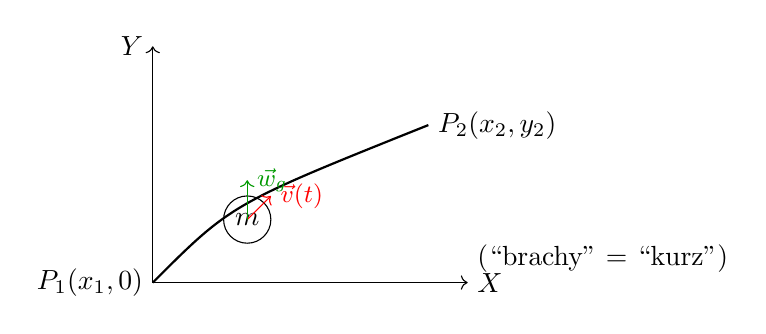
\begin{tikzpicture}
\draw[->] (0,0) -- (4,0) node[right] {$X$} node[above right] {(``brachy'' = ``kurz'')};
\draw[->] (0,0) -- (0,3) node[left] {$Y$};
\draw (0,0) node[left] {$P_1(x_1,0)$};
\draw (3.5,2) node[right] {$P_2(x_2,y_2)$};
\draw[thick] (0,0) .. controls (1,1) .. (3.5,2);
\draw (1.2,0.8) circle (0.3) node {$m$};
\draw[->,red] (1.2,0.8) -- (1.5,1.1) node[right] {\small $\vec{v}(t)$};
\draw[->,green!60!black] (1.2,0.8) -- (1.2,1.3) node[right] {\small $\vec{w}_g$};
\end{tikzpicture}
\end{center}

\textbf{Problemstellung:} Ein Massenpunkt $m$ mit Anfangsgeschwindigkeit null soll sich reibungsfrei im homogenen Gravitationsfeld von $P_1 = (x_1, 0)$ nach $P_2 = (x_2, y_2)$ bewegen. Gesucht ist die Kurve $y(x)$, auf der die benötigte Zeit $T$ minimal ist.

\textbf{Herleitung des Zeitfunktionals:} Die Bahngeschwindigkeit ist gegeben durch:
\[
\|\vec{v}(t)\| = \frac{ds}{dt} \quad \Rightarrow \quad dt = \frac{ds}{v}
\]
mit Bogenlängenelement:
\[
ds = \sqrt{dx^2 + dy^2} = dx \cdot \sqrt{1 + \left( \frac{dy}{dx} \right)^2}
\]
Daraus folgt:
\[
T = \int_{P_1}^{P_2} \frac{ds}{v} = \int_{x_1}^{x_2} \frac{\sqrt{1 + y'^2}}{v} dx
\]

\textbf{Energieerhaltung:} Aus der Energieerhaltung folgt:
\[
\frac{1}{2}mv^2 = mgy \quad \Rightarrow \quad v = \sqrt{2gy}
\]
Daher ergibt sich das Funktional:
\[
T[y] = \int_{x_1}^{x_2} \frac{\sqrt{1 + (y')^2}}{\sqrt{2gy}}\, dx
= \frac{1}{\sqrt{2g}} \int_{x_1}^{x_2} \frac{\sqrt{1 + (y')^2}}{\sqrt{y}}\, dx
\]

\textbf{Euler-Lagrange-Gleichung:} Definiere:
\[
F(y, y') = \frac{1}{\sqrt{2g}} \cdot \frac{\sqrt{1 + (y')^2}}{\sqrt{y}}
\]
Dann liefert die Euler-Lagrange-Gleichung:
\[
\frac{\partial F}{\partial y} - \frac{d}{dx} \left( \frac{\partial F}{\partial y'} \right) = 0
\]

\textbf{Erhaltungsgröße:} Da $F$ nicht explizit von $x$ abhängt, ist die Hamilton-Funktion
\[
H = \frac{\partial F}{\partial y'} \cdot y' - F
\]
entlang Lösungen der Euler-Lagrange-Gleichung konstant.

\textbf{Lösung — Zykloide:} Die Lösung des Problems ist eine Zykloide mit Parameterdarstellung:
\[
\begin{pmatrix} x - x_0 \\ y \end{pmatrix}
= r_0 \begin{pmatrix} \varphi - \sin\varphi \\ 1 - \cos\varphi \end{pmatrix}
\]
Dies entspricht der Bahnkurve eines Punktes auf dem Rand eines rollenden Rades.

Der Parameter $r_0$ wird so gewählt, dass die Kurve durch den Zielpunkt $P_2 = (x_2, y_2)$ verläuft.



\subsubsection{Das Hamiltonsche Prinzip} 

Darunter versteht man die folgende Aussage (auch genannt ``Prinzip der stationären Wirkung''):

Die Bewegung eines mechanischen Systems von einem gegebenen Anfangspunkt zur Zeit $t_1$ zu einem gegebenen Endpunkt zur Zeit $t_2$ verläuft so, dass die Wirkung $S$ stationär ist,

\[\delta S = 0, \quad S = \int_{t_1}^{t_2} dt\, L(q(t), \dot{q}(t), t)\]

Dies ist die kompakteste Formulierung der klassischen Mechanik: in $\delta S = 0$ ist dieselbe Physik wie in den Lagrange-gleichungen enthalten. Viele Lehrbücher benutzen daher das Hamiltonsche Prinzip als Ausgangspunkt zum formalen Aufbau der Mechanik. Es gilt sowohl für holonome Z.B. als auch für differenzielle Z.B., solange sich die Kräfte aus generalisierten Potentialen herleiten lassen.


\textbf{Für holonome Z.B.} lassen sich die Lagrangegleichungen aus dem Hamiltonschen Prinzip direkt mit Hilfe der Regeln der Variationsrechnung beweisen:

\[\delta S = \sum_{j=1}^n \int_{t_1}^{t_2} dt\, \left[\frac{\partial L}{\partial q_j} - \frac{d}{dt}\frac{\partial L}{\partial \dot{q}_j}\right]\delta q_j, \quad \delta q_j(t_1) = 0 = \delta q_j(t_2)\]

Da die $q_j$ unabhängig sind folgt 
$$\frac{\partial L}{\partial q_j} - \frac{d}{dt}\frac{\partial L}{\partial \dot{q}_j} = 0$$
Die Euler-Lagrangegleichungen des Variationsproblems für $S$ sind genau die Lagrangegleichungen 2. Art.

Das Hamiltonsche Prinzip gilt auch für Systeme mit differentiellen Zwangsbedingungen: (ZB), d.\,h. Nebenbedingungen der Form
\[
\sum_{i=1}^M q_{ji}(q,\dot{q},t)\, \delta q_i + q_{jt}(q,\dot{q},t)\, \delta t = 0, \quad j = 1,\dots,k
\]
Im autonomen Fall (feste Zeit $t$) vereinfacht sich dies zu
\[
\sum_{i=1}^M q_{ji}\, \delta q_i = 0, \quad j=1,\dots,k
\]
Die Variationen $\delta q_i$ sind also nicht mehr unabhängig. Um diese Einschränkungen im Hamiltonschen Prinzip zu berücksichtigen, führt man zeitabhängige Lagrange-Multiplikatoren $\lambda_j(t)$ ein und betrachtet stattdessen
\[
\sum_{j=1}^k \lambda_j(t) \sum_{i=1}^M q_{ji}\, \delta q_i = \sum_{i=1}^M \left( \sum_{j=1}^k \lambda_j q_{ji} \right)\delta q_i
\]
Damit ergibt sich für die Variation der Wirkung:
\[
\delta S = \sum_{i=1}^M \int_{t_1}^{t_2} dt\, \left[ \frac{\partial L}{\partial q_i} - \frac{d}{dt} \frac{\partial L}{\partial \dot{q}_i} + \sum_{j=1}^k \lambda_j q_{ji} \right] \delta q_i = 0
\]
Da nun die $\delta q_i$ als formal unabhängig gelten (durch die Erweiterung mit Lagrange-Multiplikatoren), folgt:
\[
\frac{d}{dt} \frac{\partial L}{\partial \dot{q}_i} - \frac{\partial L}{\partial q_i} = \sum_{j=1}^k \lambda_j q_{ji}
\]
Dies sind die \textbf{Lagrangegleichungen 1. Art}, wobei die $\lambda_j$ die Zwangskräfte darstellen, die aus den Nebenbedingungen resultieren.





\textbf{Anmerkungen:}

\begin{enumerate}
    \item $\delta S = 0$ impliziert nicht notwendigerweise, dass $S$ ein Minimum ist — häufig ist das jedoch der Fall.
    
    \item Durch das Hamiltonsche Prinzip werden die Bahnen nicht durch die $2n = 2(M - k)$ Anfangswerte $(q_j(t_1), \dot{q}_j(t_1))_{j=1,\dots,n}$ festgelegt, sondern durch die Randwerte der Koordinaten zu den Zeiten $t_1$ und $t_2$: $q_j(t_1), q_j(t_2)$ für $j = 1,\dots,n$.
    
    \item Die Wirkung $S = \int dt\, L$ spielt eine zentrale Rolle in der auf dem Pfadintegral basierenden Feynmanschen Formulierung der Quantenmechanik.
\end{enumerate}






\pagebreak

\section{Teil II: Anwendungen der Lagrangeschen Mechanik}

\subsection{Kinematik des starren Körpers}


In Mechanik I (Kapitel 8) haben wir die Rotation eines starren Körpers um eine feste Achse untersucht; in diesem Fall gibt es eine formale Analogie zur linearen Bewegung. Ist der Körper jedoch gar nicht oder nur an einem einzigen Punkt fixiert, so ist die Bewegung viel komplizierter. Im folgenden Kapitel 8 werden wir dieses Problem mit Hilfe des Lagrange-Formalismus untersuchen. Zunächst müssen wir jedoch geeignete generalisierte Koordinaten finden, um die Kinematik eines starren Körpers zu beschreiben. Wir erinnern dazu an den Satz von Chasle (siehe Mechanik I, Kap. 8.1, S.204):

Die allgemeine Bewegung eines starren Körpers lässt sich zerlegen in
\begin{enumerate}
\item Translation eines beliebigen Punktes
\item Rotation um diesen Punkt.
\end{enumerate}

\subsubsection{Kinetische Energie, Drehimpuls, Trägheitstensor}


Gegeben sei ein starrer Körper mit $N$ Massen $m_i$ ($i = 1,\dots,N$), Gesamtmasse $M = \sum_{i=1}^N m_i$. Nach König’s Theorem (vgl. Mech.I, S.165) lässt sich die kinetische Energie des Körpers in einen Translations- und Relativanteil zerlegen:
\[
T = \underbrace{\frac{M}{2} \vec{V}_{CM}^2}_{T_{\text{trans}}} + \underbrace{\frac{1}{2} \sum_{i=1}^N m_i \dot{\vec{r}}_i^2}_{T_{\text{rel}}}, \quad \vec{V}_{CM} = \dot{\vec{R}}_{CM}
\]
wobei $\vec{R}_{CM}$ der Schwerpunktvektor im Inertialsystem ist und $\vec{r}_i'$ die Position von Masse $m_i$ im Schwerpunktsystem bezeichnet.

Der Gesamtdrehimpuls bezüglich eines Ursprungs im Inertialsystem ist ebenfalls in Schwerpunkt- und Relativanteil zerlegbar (Mech.I, S.178):
\[
\vec{L} = \vec{R}_{CM} \times M \dot{\vec{R}}_{CM} + \sum_{i=1}^N \vec{r}_i' \times m_i \dot{\vec{r}}_i'
\]
Im Fall eines fixierten Körpers ist es sinnvoll, den Ursprung in den Fixpunkt zu legen; für einen freibeweglichen Körper liegt der Ursprung meist im Schwerpunkt. In beiden Fällen bleibt nur der Relativanteil übrig:
\[
T = T_{\text{rot}} = \sum_{i=1}^N \frac{m_i}{2} \dot{\vec{r}}_i^2, \qquad
\vec{L} = \sum_{i=1}^N \vec{r}_i \times m_i \dot{\vec{r}}_i
\]
Dabei bezeichnet $\vec{r}_i$ nun die Position relativ zum gewählten Ursprung. Für einen starren Körper rotiert $\vec{r}_i$ um diesen Ursprung, also gilt
\[
\dot{\vec{r}}_i = \vec{\omega}(t) \times \vec{r}_i(t)
\]
mit $\vec{\omega}(t)$ als Winkelgeschwindigkeitsvektor (Mech. I, S.206). Wir wenden nun die BAC–CAB-Regel an:
\[
\begin{aligned}
\vec{L} &= \sum_{i=1}^N m_i \vec{r}_i \times (\vec{\omega} \times \vec{r}_i)
= \sum_{i=1}^N m_i \left( \vec{\omega} r_i^2 - \vec{r}_i (\vec{r}_i \cdot \vec{\omega}) \right) \\
T_{\text{rot}} &= \sum_{i=1}^N \frac{m_i}{2} (\vec{\omega} \times \vec{r}_i)^2
= \frac{1}{2} \sum_{i=1}^N m_i \left( \vec{\omega}^2 r_i^2 - (\vec{\omega} \cdot \vec{r}_i)^2 \right)
\end{aligned}
\]
Ein Vergleich ergibt:
\[
\boxed{T_{\text{rot}} = \frac{1}{2} \vec{\omega} \cdot \vec{L}}
\]
Für die Darstellung in der Basis $\{ \vec{e}_1, \vec{e}_2, \vec{e}_3 \}$ definieren wir:
\[
L_\alpha = \vec{e}_\alpha \cdot \vec{L}, \quad r_{i,\alpha} = \vec{e}_\alpha \cdot \vec{r}_i, \quad \omega_\alpha = \vec{e}_\alpha \cdot \vec{\omega}, \quad \alpha = 1,2,3
\]
Im Inertialsystem werden die Vektoren $\vec{L}$, $\vec{r}_i$ und $\vec{\omega}$ dann durch die folgenden Spaltenvektoren dargestellt:
\[
\underset{\sim}{\vec{L}} =
\begin{pmatrix}
L_1 \\
L_2 \\
L_3
\end{pmatrix}
=
\begin{pmatrix}
\vec{e}_1 \cdot \vec{L} \\
\vec{e}_2 \cdot \vec{L} \\
\vec{e}_3 \cdot \vec{L}
\end{pmatrix}, \qquad
\underset{\sim}{\vec{r}_i} =
\begin{pmatrix}
r_{i,1} \\
r_{i,2} \\
r_{i,3}
\end{pmatrix}, \qquad
\underset{\sim}{\vec{\omega}} =
\begin{pmatrix}
\omega_1 \\
\omega_2 \\
\omega_3
\end{pmatrix}
\]
Dann ist
\[
\begin{aligned}
L_\alpha &= \sum_{i=1}^N m_i \left( \omega_\alpha r_i^2 - r_{i,\alpha} \sum_{\beta=1}^3 r_{i,\beta} \omega_\beta \right) \\
&= \sum_{\beta=1}^3 \left[ \sum_{i=1}^N m_i \left( r_i^2 \delta_{\alpha\beta} - r_{i,\alpha} r_{i,\beta} \right) \right] \omega_\beta
= \sum_{\beta=1}^3 I_{\alpha\beta} \omega_\beta
\end{aligned}
\]
wobei Trägheitstensor im Inertialsystem in ausgewählten Basis $\vec{e}_1, \vec{e}_2, \vec{e}_3$ definiert als durch
$$
\begin{aligned}
I_{\alpha\beta} = \sum_{i=1}^N m_i \left(\delta_{\alpha\beta} r_i^2 - r_{i\alpha} r_{i\beta}\right)
\end{aligned}
$$
Die entsprechende 3$\times$3-Matrix:
$$
\begin{aligned}
I = \begin{pmatrix}
I_{11} & I_{12} & I_{13} \\
I_{21} & I_{22} & I_{23} \\
I_{31} & I_{32} & I_{33}
\end{pmatrix}
\end{aligned}
$$
nennt man Darstellung des Trägheitstensors in der Basis $\vec{e}_1,\vec{e}_2,\vec{e}_3$.

(Genau wie Vektoren sind Tensoren durch ihr Transformations-Verhalten bei Drehungen definiert und sind als absolute Objekte unabhängig von einer konkreten Basis. Man unterscheidet daher zwischen absoluten Tensoren und ihren Basis-Darstellungen).

In Matrix-Schreibweise können wir den Zusammenhang $L_\alpha = \sum_\beta I_{\alpha\beta}w_\beta$ auch so schreiben:
$$
\begin{aligned}
\vec{\underset{\sim}{L}} = I \vec{\underset{\sim}{w}}, \quad I = \sum_{i=1}^N m_i \begin{bmatrix}
1 & 0 & 0 \\
0 & 1 & 0 \\
0 & 0 & 1
\end{bmatrix} \vec{\underset{\sim}{r}}_i \vec{\underset{\sim}{r}}_i^T - \vec{\underset{\sim}{r}}_i \vec{\underset{\sim}{r}}_i^T
\end{aligned}
$$
Analog ergibt sich für die kinetische Energie der Rotation:
$$
\begin{aligned}
T_{rot} = \frac{1}{2} \vec{\underset{\sim}{w}}^T \vec{\underset{\sim}{L}} = \frac{1}{2} \vec{\underset{\sim}{w}}^T I \vec{\underset{\sim}{w}}
\end{aligned}
$$



\textbf{Anmerkung:} Bei kontinuierlicher Massenverteilung mit Dichte $\rho(\vec{r})$:

$$
\begin{aligned}
I_{\alpha\beta} = \int d^3r \rho(\vec{r}) \left[\delta_{\alpha\beta} \vec{r}^2 - (\vec{e}_\alpha \cdot \vec{r})(\vec{e}_\beta \cdot \vec{r})\right]
\end{aligned}
$$


\subsubsection{Transformation ins körperfeste (rotierende) Bezugsystem}

Die Beschreibung der Bewegung eines starren Körpers ist oft einfacher, wenn man in einem körperfesten Bezugssystem arbeitet, dessen Achsen der Rotationsbewegung des Körpers folgen. Ist der Körper in einem Punkt fixiert, so legen wir den Ursprung des körperfesten Bezugssystems – wie auch den des zugehörigen Inertialsystems – in diesen Punkt:

\begin{center}
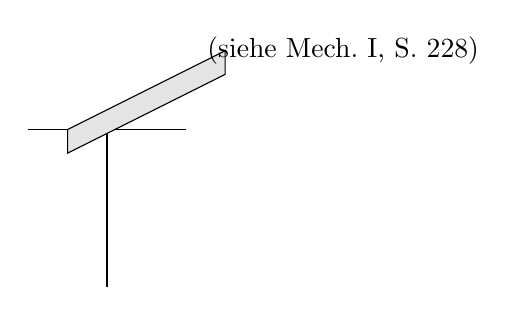
\begin{tikzpicture}
\draw (0,-1) -- (0,1);
\draw (-1,1) -- (1,1);
\draw[red] (0,1) -- (1.5,2);
\draw[fill=gray!20] (-0.5,1) -- (1.5,2) -- (1.5,1.7) -- (-0.5,0.7) -- cycle;
\node at (3,2) {(siehe Mech.~I, S.~228)};
\end{tikzpicture}
\end{center}

Ist der Körper hingegen nicht fixiert, so wählen wir den Ursprung des körperfesten Systems im Schwerpunkt:

\begin{center}
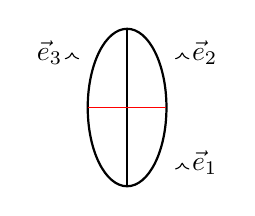
\begin{tikzpicture}
\draw[thick] (0,0) circle (0.5 and 1);
\draw[thick] (0,1) -- (0,-1);
\draw[red] (-0.5,0) -- (0.5,0);
\draw[->] (0.7,0.7) node[right] {$\vec{e}_2$};
\draw[->] (-0.7,0.7) node[left] {$\vec{e}_3$};
\draw[->] (0.7,-0.7) node[right] {$\vec{e}_1$};
\end{tikzpicture}
\end{center}

Alle Vektoren müssen nun auf die zeitabhängige Basis des körperfesten Bezugssystems projiziert werden. Den Übergang vom Inertialsystem in ein beschleunigtes (hier rotierendes) Bezugssystem haben wir bereits in Mechanik~I (Kapitel~4.8) diskutiert. Für die Koordinatendarstellungen gelten dann die Transformationsgleichungen:
\[
\underline{r}' = R \underline{r}, \qquad
\underline{\omega}' = R \underline{\omega}, \qquad
\underline{L}' = R \underline{L}
\]
(siehe Mech.~I, S.~205f.)

Dabei ist $R(t)$ die zeitabhängige Rotationsmatrix, die das Inertialsystem mit dem körperfesten Bezugssystem verbindet (vgl. Mech.~I, S.~26):
\[
R_{\alpha\beta}(t) = \vec{e}'_\alpha(t) \cdot \vec{e}_\beta, \qquad
\vec{e}'_\alpha(t) = \sum_{\beta=1}^3 R_{\alpha\beta}(t) \vec{e}_\beta
\]

Mit $\vec{\underset{\sim}{L}} = I \vec{\omega}$ ergibt sich:
\[
\vec{\underset{\sim}{L}}' = R \vec{\underset{\sim}{L}} = R I \vec{\underset{\sim}{\omega}} = R I R^{-1} \vec{\underset{\sim}{\omega}}' = I' \vec{\underset{\sim}{\omega}}' \qquad \Rightarrow \qquad \vec{\underset{\sim}{L}}' = I' \vec{\underset{\sim}{\omega}}', \quad \text{mit } I' = R I R^{-1}
\]
Analog folgt für die Rotationsenergie:
\[
T_{\text{rot}} = \frac{1}{2} \vec{\underset{\sim}{\omega}}'^{\,T} I' \vec{\underset{\sim}{\omega}}'
\]

Der transformierte Trägheitstensor $I'$ hat formal dieselbe Struktur wie $I$, jedoch mit neuen Komponenten:
\[
r_{i,\alpha}(t) = \vec{e}_\alpha \cdot \vec{r}_i(t)
\quad \Rightarrow \quad
r'_{i,\alpha}(t) = \vec{e}'_\alpha(t) \cdot \vec{r}_i(t)
\]

Im körperfesten System sind die $r'_{i,\alpha}(t)$ zeitunabhängig, d.\,h. $r'_{i,\alpha}(t) = r'_{i,\alpha}(0)$, daher ist auch $I'$ zeitlich konstant.

Das Transformationsverhalten des Trägheitstensors beim Wechsel in ein rotierendes Koordinatensystem ist:
\[
I' = R I R^{-1}
\]
bzw. komponentenweise:
\[
\begin{aligned}
I'_{\alpha\beta} &= \sum_{\alpha_1, \alpha_2} R_{\alpha \alpha_1} I_{\alpha_1 \alpha_2} (R^{-1})_{\alpha_2 \beta} \\
&= \sum_{\alpha_1, \alpha_2} R_{\alpha \alpha_1} R_{\beta \alpha_2} I_{\alpha_1 \alpha_2}
\end{aligned}
\]
Dies ist die definierende Eigenschaft eines (Koordinaten-)Tensors. Jede Matrix, die sich bei Rotationen gemäß dieser Vorschrift transformiert, verdient den Namen „Darstellung eines Tensors“.










\section*{Hauptträgheitsachsen}

In der Praxis ist es oft günstig, die Körperfesten Basisvektoren $\vec{e}_1'$, $\vec{e}_2'$, $\vec{e}_3'$ so zu wählen dass die Darstellung des Trägheitstensors $I'$ in der Körperfesten Basis diagonal ist.

\[
I' = R I R^T = \begin{pmatrix}
I_1' & 0 & 0 \\
0 & I_2' & 0 \\
0 & 0 & I_3'
\end{pmatrix}
\]

\[ \Rightarrow L_\alpha' = I_\alpha' \omega_\alpha', \alpha = 1,2,3, \quad T_{rot} = \frac{1}{2}(I_1'\omega_1'^2 + I_2'\omega_2'^2 + I_3'\omega_3'^2) \]

\noindent
Man nennt:
\begin{itemize}
\item $\vec{e}_\alpha'$: Richtungen der Hauptträgheitsachsen
\item $I_\alpha'$: Hauptträgheitsmomente
\end{itemize}

\noindent
Spezialfälle:
\begin{itemize}
\item $I_1' \neq I_2' \neq I_3'$: unsymmetrischer Kreisel
\item $I_1' = I_2' \neq I_3'$: symmetrischer Kreisel
\item $I_1' = I_2' = I_3'$: Kugelkreisel
\item $I_1' = I_2'$, $I_3' = 0$: Rotator
\end{itemize}

Bei hinreichend symmetrischen Körpern kann man die Hauptachsen ohne Rechnung erraten, in dem man das Körperfeste Koordinatensystem der Symmetrie des Körpers anpasst!

Ist der Körper jedoch unsymmetrisch so dass man die Hauptachsen nicht erraten kann, muss man diese durch explizite Diagonalisierung des Trägheitstensors bestimmen. Das geht so:

Matrix $R$ so dass

\[
RIR^{-1} = \begin{pmatrix}
I_1' & 0 & 0 \\
0 & I_2' & 0 \\
0 & 0 & I_3'
\end{pmatrix} \Leftrightarrow IR^{-1} = R^{-1} \begin{pmatrix}
I_1' & 0 & 0 \\
0 & I_2' & 0 \\
0 & 0 & I_3'
\end{pmatrix}
\]

mit $(R^{-1})_{\alpha\beta} = R_{\beta\alpha} = \vec{e}_\beta \cdot \vec{e}_\alpha' = \vec{e}_\alpha' \cdot \vec{e}_\beta$ lautet diese Gleichung in Komponentenschreibweise:

\[
\sum_{k=1}^3 I_{\alpha k}(R^{-1})_{k\beta} = (R^{-1})_{\alpha\beta}I_\beta' \Leftrightarrow I\vec{\underset{\sim}{e}}_\beta' = I_\beta'\vec{\underset{\sim}{e}}_\beta', \quad \vec{\underset{\sim}{e}}_\beta' = \begin{pmatrix}
\vec{e}_1 \cdot \vec{e}_\beta' \\
\vec{e}_2 \cdot \vec{e}_\beta' \\
\vec{e}_3 \cdot \vec{e}_\beta'
\end{pmatrix}
\]
Man nennt die $\vec{\underset{\sim}{e}}_\beta'$ die Eigenvektoren von $I$; die $I_\beta'$ heißen die zugehörigen Eigenwerte. Wie man solche linearen Eigenwertgleichungen explizit löst lernt man in der linearen Algebra.



\subsection*{Anmerkungen:}
\begin{enumerate}
  \item Der Trägheitstensor hat die nette Eigenschaft $I_{\alpha\beta} = I_{\beta\alpha}$, d.h., er ist reell und symmetrisch. Daraus folgt:
  \begin{enumerate}
    \item Alle Eigenwerte $I_\alpha'$ sind reell.
    \item Die Eigenvektoren $\vec{e}_\alpha'$ können so gewählt werden, dass sie eine Orthonormalbasis bilden.
  \end{enumerate}
  
  \item Im Hauptachsensystem gilt $L_\alpha' = I_\alpha'\omega_\alpha'$, d.h. $\vec{L}$ und $\vec{\omega}$ sind genau dann parallel, wenn der Körper um eine Hauptachse rotiert.

  \item Rotiert der Körper um eine feste Achse in Richtung eines Einheitsvektors $\vec{n}$ im Inertialsystem, so ist
  \[
  I_{\underset{\sim}{n}} = \vec{\underset{\sim}{n}}^T I \vec{\underset{\sim}{n}}
  \]
  das zugehörige Trägheitsmoment.
\end{enumerate}




\subsubsection{Die Eulerschen Winkel}

Diese bilden einen Satz von unabhängigen generalisierten Koordinaten, die die Lage des starren Körpers relativ zum Ursprung des Inertialsystems (Schwerpunkt bzw. der fixierte Punkt des starren Körpers) eindeutig festlegen. Wegen

\[
\vec{e}_i'(t) = \sum_{j=1}^3 R_{ij}(t) \vec{e}_j \quad \text{(siehe S. 30, mit }\alpha,\beta,\gamma\text{)}
\]

\noindent
müssen wir dazu die Drehmatrix $R_{ij}(t)$ geeignet parametrisieren. Da hier keine Verwechslung mit dem Teilchenindex i auftreten kann, nennen wir den Komponentenindex wieder $\alpha \to i$, $\beta \to j$.

Die Eulerschen Winkel stellen eine mögliche Parametrisierung dar: es sind Drehwinkel in 3 verschiedenen Koordinatensystemen, welche durch die Eulerschen Winkel selbst definiert sind.

Wir zerlegen dazu die durch $R(t)$ beschriebene Drehung in 3 Schritte:

\begin{center}
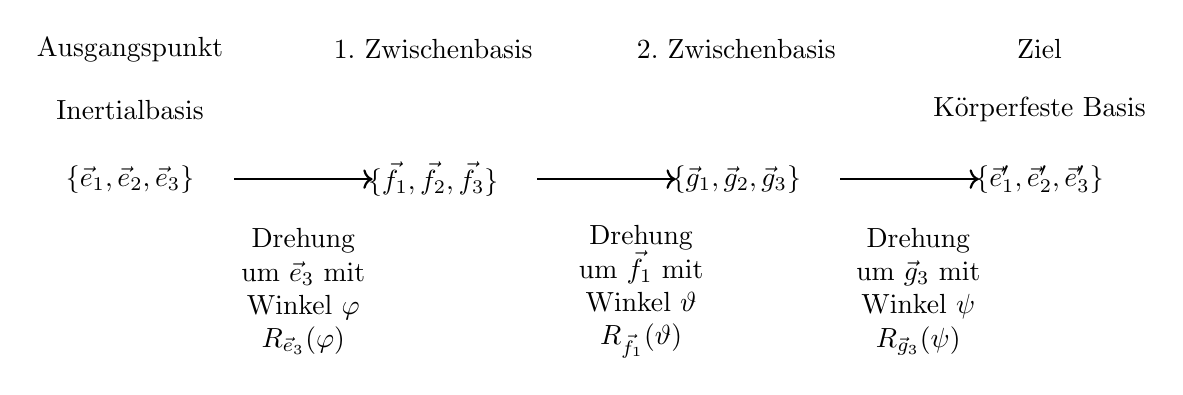
\begin{tikzpicture}[every node/.style={font=\normalsize}, scale=1.1]
% Tabellenüberschriften
\node at (0,4) {Ausgangspunkt};
\node at (3.5,4) {1.~Zwischenbasis};
\node at (7,4) {2.~Zwischenbasis};
\node at (10.5,4) {Ziel};

% Basenbezeichnungen
\node at (0,3.3) {Inertialbasis};
\node at (10.5,3.3) {Körperfeste Basis};

% Basisvektoren
\node at (0,2.5) {$\{\vec{e}_1, \vec{e}_2, \vec{e}_3\}$};
\node at (3.5,2.5) {$\{\vec{f}_1, \vec{f}_2, \vec{f}_3\}$};
\node at (7,2.5) {$\{\vec{g}_1, \vec{g}_2, \vec{g}_3\}$};
\node at (10.5,2.5) {$\{\vec{e}_1', \vec{e}_2', \vec{e}_3'\}$};

% Pfeile zwischen Basen
\draw[->, thick] (1.2,2.5) -- (2.8,2.5);
\draw[->, thick] (4.7,2.5) -- (6.3,2.5);
\draw[->, thick] (8.2,2.5) -- (9.8,2.5);

% Beschreibung der Rotationen
\node[align=center] at (2,1.2) {Drehung\\ um $\vec{e}_3$ mit\\ Winkel $\varphi$\\ $R_{\vec{e}_3}(\varphi)$};
\node[align=center] at (5.9,1.2) {Drehung\\ um $\vec{f}_1$ mit\\ Winkel $\vartheta$\\ $R_{\vec{f}_1}(\vartheta)$};
\node[align=center] at (9.1,1.2) {Drehung\\ um $\vec{g}_3$ mit\\ Winkel $\psi$\\ $R_{\vec{g}_3}(\psi)$};

\end{tikzpicture}
\end{center}
Für die Drehmatrizen ergeben sich die folgenden expliziten Darstellungen:
\noindent

1. Drehung:
\[\vec{f}_i = \sum_{j=1}^3 (R_{\vec{e}_3}(\varphi))_{ij}\vec{e}_j\]

\[R_{\vec{e}_3}(\varphi) = \begin{pmatrix}
\cos\varphi & \sin\varphi & 0 \\
-\sin\varphi & \cos\varphi & 0 \\
0 & 0 & 1
\end{pmatrix}\]

\noindent
2. Drehung:
\[\vec{g}_i = \sum_{j=1}^3 (R_{\vec{f}_1}(\vartheta))_{ij}\vec{f}_j\]

\[R_{\vec{f}_1}(\vartheta) = \begin{pmatrix}
1 & 0 & 0 \\
0 & \cos\vartheta & \sin\vartheta \\
0 & -\sin\vartheta & \cos\vartheta
\end{pmatrix}\]

\noindent
3. Drehung:
\[\vec{e}_i' = \sum_{j=1}^3 (R_{\vec{g}_3}(\psi))_{ij}\vec{g}_j\]

\[R_{\vec{g}_3}(\psi) = \begin{pmatrix}
\cos\psi & \sin\psi & 0 \\
-\sin\psi & \cos\psi & 0 \\
0 & 0 & 1
\end{pmatrix}\]






Geometrische Interpretation der Eulerschen Winkel

\begin{figure}[h]
\centering
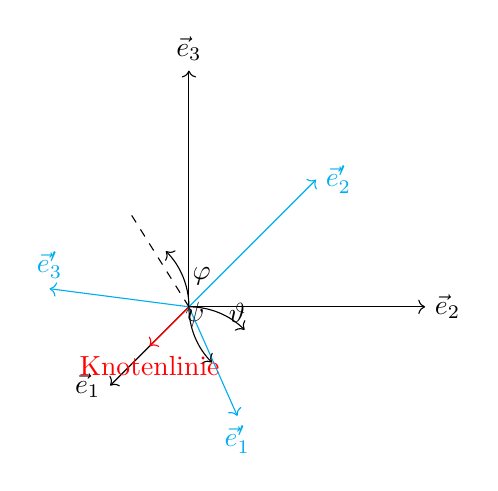
\begin{tikzpicture}
\draw[->] (0,0,0) -- (3,0,0) node[right] {$\vec{e}_2$};
\draw[->] (0,0,0) -- (0,3,0) node[above] {$\vec{e}_3$};
\draw[->] (0,0,0) -- (-1,-1,0) node[left] {$\vec{e}_1$};

\draw[->, color=cyan] (0,0,0) -- (2,2,1) node[right] {$\vec{e}_2'$};
\draw[->, color=cyan] (0,0,0) -- (-1,1,2) node[above] {$\vec{e}_3'$};
\draw[->, color=cyan] (0,0,0) -- (1,-1,1) node[below] {$\vec{e}_1'$};

\draw[red, ->] (0,0,0) -- (-0.5,-0.5,0) node[below] {Knotenlinie};

\draw[->] (0,0,0) arc (0:45:1) node[pos=0.5, right] {$\varphi$};
\draw[dashed] (0,0,0) -- (0,2,2);
\draw[->] (0,0,0) arc (90:45:1) node[pos=0.5, right] {$\vartheta$};
\draw[->] (0,0,0) arc (180:225:1) node[pos=0.5, above] {$\psi$};

\end{tikzpicture}
\end{figure}

Die Eulerwinkel legen die Orientierung des körperfesten Systems $\{\vec{e}_1', \vec{e}_2', \vec{e}_3'\}$ relativ zum Inertialsystem $\{\vec{e}_1, \vec{e}_2, \vec{e}_3\}$ eindeutig fest:

$\varphi,\vartheta$: geben Stellung der körperfesten $\vec{e}_3'$-Achse (``Figurenachse'') im Inertialsystem an.

$\psi$: beschreibt Drehung von $\vec{e}_3'$-Achse.

Man nennt: \quad $\varphi$: Präzessionswinkel; $\vartheta$: Nutationswinkel; $\psi$: Eigenrotationswinkel.

Mit der expliziten Parametrisierung auf S. 54 ergibt sich für die Gesamtdrehung:
\[\vec{e}_i' = \sum_{j,k,\ell=1}^3 [R_{\vec{g}_3}(\psi)]_{ij} [R_{\vec{f}_1}(\vartheta)]_{jk} [R_{\vec{e}_3}(\varphi)]_{k\ell} \vec{e}_\ell = \sum_{\ell=1}^3 R_{i\ell}(\varphi,\vartheta,\psi)\vec{e}_\ell\]

mit 
\[R(\varphi,\vartheta,\psi) = R_{\vec{g}_3}(\psi) R_{\vec{f}_1}(\vartheta) R_{\vec{e}_3}(\varphi)\]

Einsetzen der expliziten Darstellungen ergibt einen ziemlich länglichen Ausdruck, den wir hier nicht reproduzieren wollen.

Um später die Lagrange Funktion des starren Körpers durch die Eulerwinkel (sowie deren Ableitungen $\dot{\varphi}$, $\dot{\vartheta}$, $\dot{\psi}$) auszudrücken, brauchen wir wegen

\[T_{rot} = \frac{1}{2} \vec{\underset{\sim}{\omega}}^T I' \vec{\underset{\sim}{\omega}}\]

jedoch den Zusammenhang zwischen den körperfesten Komponenten $\omega_i$ der Winkelgeschwindigkeit und den Eulerwinkeln:

Aus der Vorlesung Mechanik I (Kapitel 4: Beschleunigte Bezugssysteme, S.98) wissen wir, dass für jede feste Drehmatrix $R(t)$ die Winkelgeschwindigkeiten $\omega_i(t)$ im beschleunigten (körperfesten) Bezugssystem gegeben sind durch:

\[\Omega_{ij}' = (\dot{R}R^T)_{ij} = \sum_k \epsilon_{ijk} \omega_k^\prime\]

Mit 
$$\dot{R} = R_{\vec{g}_3}(\psi) R_{\vec{f}_1}(\vartheta) \dot{R}_{\vec{e}_3}(\varphi) + R_{\vec{g}_3}(\psi) \dot{R}_{\vec{f}_1}(\vartheta) R_{\vec{e}_3}(\varphi) + \dot{R}_{\vec{g}_3}(\psi) R_{\vec{f}_1}(\vartheta) R_{\vec{e}_3}(\varphi)$$
$$R^T = \hat{R} = R_{\vec{e}_3}^T(\varphi) R_{\vec{f}_1}^T(\vartheta) R_{\vec{g}_3}^T(\psi)$$
Es folgt
\[\Omega' = \dot{R}R^T = R_{\vec{g}_3}(\psi) \dot{R}_{\vec{g}_3}^T(\psi) + R_{\vec{g}_3}(\psi)R_{\vec{f}_1}(\vartheta) \dot{R}_{\vec{f}_1}^T(\vartheta) R_{\vec{g}_3}^T(\psi)\]
\[+ R_{\vec{g}_3}(\psi) R_{\vec{f}_1}(\vartheta) \dot{R}_{\vec{e}_3}(\varphi) R_{\vec{e}_3}^T(\varphi) R_{\vec{f}_1}^T(\vartheta) R_{\vec{g}_3}^T(\psi).\]
Im Prinzip können wir nun die Matrizen ausmultiplizieren und dann aus $\Omega_{ij}' = \sum_k \epsilon_{ijk} \omega_k'$ die $\omega_k'$ als Funktion von $\dot{\varphi}$, $\dot{\vartheta}$, $\dot{\psi}$ berechnen.

Vereinfachung der Rechnung: benutze Äquivalenz der antisymmetrischen Matrix $\Omega'$ mit $\vec{\underset{\sim}{\omega}}'$ sowie die Matrix-Gleichung (siehe Mech. I, Kapitel 8, S. 289)

\[\Omega' = R \Omega R^{-1} \text{ mit } \underset{\sim}{\omega}' = R \underset{\sim}{\omega}\]
Und damit: $R_{\vec{g}_3}(\psi) R_{\vec{g}_3}^T(\psi)$ entspricht $\vec{\underset{\sim}{\omega}}_{\psi}' = \begin{pmatrix} 0 \\ 0 \\ \dot{\psi} \end{pmatrix}$
$$R_{\vec{g}_3}(\psi) R_{\vec{f}_1}(\vartheta) R_{\vec{f}_1}^T(\vartheta) R_{\vec{g}_3}^T(\psi) \text{ entspricht }
\vec{\omega}_\vartheta' = R_{\vec{g}_3}(\psi) \begin{pmatrix} \dot{\vartheta} \\ 0 \\ 0 \end{pmatrix} = \begin{pmatrix} \cos\psi \dot{\vartheta} \\ -\sin\psi \dot{\vartheta} \\ 0 \end{pmatrix}$$
$R_{\vec{g}_3}(\psi) R_{\vec{f}_1}(\vartheta) R_{\vec{e}_3}(\varphi) R_{\vec{e}_3}^T(\varphi) R_{\vec{f}_1}^T(\vartheta) R_{\vec{g}_3}^T(\psi)$ entspricht:
$$\vec{\omega}_\varphi' = R_{\vec{g}_3}(\psi) R_{\vec{f}_1}(\vartheta) \begin{pmatrix} 0 \\ 0 \\ \dot{\varphi} \end{pmatrix} = R_{\vec{g}_3}(\psi) \begin{pmatrix} \sin\vartheta \dot{\varphi} \\ \cos\vartheta \dot{\varphi} \\ 0 \end{pmatrix} = \begin{pmatrix} \sin\vartheta \sin\psi \dot{\varphi} \\ \cos\psi \sin\vartheta \dot{\varphi} \\ \cos\vartheta \dot{\varphi} \end{pmatrix}$$
Insgesamt ergibt sich damit folgender Zusammenhang zwischen den körperfesten Komponenten der Winkelgeschwindigkeit und den Eulerwinkeln:
\[\vec{\underset{\sim}{\omega}}' = \vec{\underset{\sim}{\omega}}_\psi' + \vec{\underset{\sim}{\omega}}_\vartheta' + \vec{\underset{\sim}{\omega}}_\varphi' = \begin{pmatrix} \sin\psi \sin\vartheta \dot{\varphi} + \cos\psi \dot{\vartheta} \\ \cos\psi \sin\vartheta \dot{\varphi} - \sin\psi \dot{\vartheta} \\ \cos\vartheta \dot{\varphi} + \dot{\psi} \end{pmatrix}\]






\pagebreak


\subsection{Dynamik des Starren Körpers}



\subsubsection{Die Eulerschen Gleichungen}

Darunter versteht man die Newtonschen Bewegungsgleichungen für die Komponenten $\omega_i'(t) = \vec{e}_i' \cdot \vec{\omega}(t)$ der Winkelgeschwindigkeit eines starren Körpers im körperfesten (beschleunigten) Bezugssystem.

\noindent
\textbf{Ausgangspunkt:} Drehimpulssatz im Inertialsystem: (Mech. I, S. 182)

\[\frac{d}{dt} \underset{\sim}{L}(t) = \underset{\sim}{N}(t), \quad L_i = \vec{e}_i \cdot \underline{L}(t), \quad N_i = \vec{e}_i \cdot \vec{N}(t)\]
Transformation ins körperfeste Bezugssystem (siehe Mech. I, S. 208):
\[\underset{\sim}{L}'(t) = R(t)\underset{\sim}{L}(t), \quad \underset{\sim}{N}'(t) = R(t)\underset{\sim}{N}(t), \quad R(t) = \text{Rotationsmatrix}\]
Wie bereits in Kapitel 4 von Mechanik I gezeigt, müssen im körperfesten System die Zeitableitungen durch "kovariante" Ableitungen ersetzt werden (siehe Mech. I, S. 104):
\[\frac{d}{dt}\underset{\sim}{L}' + \underset{\sim}{\Omega}' \times \underset{\sim}{L}' = \underset{\sim}{N}' \quad \Leftrightarrow \quad \left(\frac{d}{dt} - \Omega'\right)\underset{\sim}{L}' = \underset{\sim}{N}'\]

wobei \[\Omega'_{ij} = \sum_k \epsilon_{ijk}\omega_k', \quad \Omega' = \begin{pmatrix} 0 & \omega_3' & -\omega_2' \\ -\omega_3' & 0 & \omega_1' \\ \omega_2' & -\omega_1' & 0 \end{pmatrix} = \dot{R}\dot{R}^{-1}\]

denn: 
\[\frac{d}{dt}\underset{\sim}{L}' = \frac{d\dot{R}(t)}{dt}\underset{\sim}{L}(t) + R(t)\frac{d\underset{\sim}{L}(t)}{dt} = \underbrace{\dot{R}(t)\dot{R}^{-1}(t)\underset{\sim}{L}'(t)}_{=\Omega'\underset{\sim}{L}'(t)} + \underbrace{R(t)\underset{\sim}{N}(t)}_{=\underset{\sim}{N}'(t)}= \Omega'\underset{\sim}{L}'(t)+\underset{\sim}{N}'(t)\]

Im Hauptachsensystem gilt also $L_i' = I_i' \omega_i'$, so dass die \textit{Eulersche Gleichungen} gelten
\begin{align*}
I_1' \dot{\omega}_1' - \omega_2' \omega_3' (I_2'-I_3') &= N_1' \\
I_2' \dot{\omega}_2' - \omega_3' \omega_1' (I_3'-I_1') &= N_2' \\
I_3' \dot{\omega}_3' - \omega_1' \omega_2' (I_1'-I_2') &= N_3'
\end{align*}





\noindent
Anmerkungen:


\begin{enumerate}
\item Spezialfall: kräftefreier Kreisel: $\underset{\sim}{N}=0=\underset{\sim}{N}'$. 
Dann bilden die Eulerschen Gleichungen ein geschlossenes System von nicht-linearen Differentialgleichungen für $\omega_i'(t)$.

\item Die Kenntnis der Winkelgeschwindigkeiten $\omega_i'$ (oder der Matrix $\Omega'=\dot{R}\hat{R}$) reicht nicht aus um die Winkellage eines Körpers zu bestimmen. Dazu brauchen wir die Matrix $R(t)$, die z.B. durch die Eulerwinkel $\varphi,\vartheta,\psi$ parametrisiert werden kann.

\item Die Dynamik eines starren Körpers im Gravitationsfeld (wo $\underset{\sim}{N}'\neq 0$) wird durch die Eulerschen Gleichungen nicht vollständig bestimmt, denn um die $N_i'(t)$ zu berechnen brauchen wir wiederum die $\omega_i'(t)$. Zur vollständigen Beschreibung der Newtonschen Dynamik eines starren Körpers im Gravitationsfeld brauchen wir noch 3 weitere Gleichungen für die Komponenten von $\underline{N}'$. Um diese herzuleiten, nehmen wir der Einfachheit halber an, dass der Körper in einem Punkt fixiert ist und sich in einem homogenen Gravitationsfeld befindet:
\begin{figure}[h]
\centering
\begin{tikzpicture}
\draw[->] (0,0) -- (2,0) node[right] {$\vec{e}_2$};
\draw[->] (0,0) -- (0,2) node[above] {$\vec{e}_3$};
\draw[->] (0,0) -- (-1,-1) node[left] {$\vec{e}_1$};
\draw[cyan,->] (0,0) -- (1,1.5) node[right] {$\vec{r}_i$};
\draw (0,0) -- (0.5,1) node[right] {$\vec{r}_{CM}$};
\end{tikzpicture}
\end{figure}
Aus Kapitel 7, Mech. I (S. 181) wissen wir:
Bei der Berechnung des Drehmoments welches ein homogenes Gravitationsfeld auf einen Körper ausübt kann man so tun, als sei die gesamte Masse des Körpers im Schwerpunkt vereint.

\end{enumerate}


Es folgt: Drehmoment auf Körper im Inertial System:
\[\underset{\sim}{N}(t) = \underset{\sim}{R}_{CM}(t) \times \underline{F}\]
Im körperfesten System gilt dann:
\[\underset{\sim}{N}'(t) = \underset{\sim}{R}'_{CM} \times \underset{\sim}{F}'(t), \text{ wobei } \underset{\sim}{F}'(t) = R(t)\underset{\sim}{F}\]
Die Bewegungsgleichung für $\underline{F}'$ ist:
\[\frac{d\underset{\sim}{F}'}{dt} = \frac{d(R(t))}{dt}\underset{\sim}{F} = \dot{R}\hat{R}^{-1}R\underset{\sim}{F} = \Omega'\underset{\sim}{F}' = -\underset{\sim}{\omega}' \times \underset{\sim}{F}'\]

Einsetzen von $\underset{\sim}{L}' = I'\underset{\sim}{\omega}'$, $I'$ zeitunabhängig.




Die vollständige Newton'sche Dynamik wird im Körperfesten System durch die folgenden 6 Gleichungen beschrieben:
\begin{equation*}
\begin{aligned}
I^\prime \dot{\underset{\sim}{\omega}}^\prime + \underset{\sim}{\omega}^\prime \times (I^\prime \underset{\sim}{\omega}^\prime) &= \underset{\sim}{R_{CM}}^\prime \times \underset{\sim}{F}^\prime \\
\dot{\underset{\sim}{F}}^\prime &= -\underset{\sim}{\omega}^\prime \times \underset{\sim}{F}^\prime
\end{aligned}
\end{equation*}

Nur im kraftfreien Fall ($\underset{\sim}{F}^\prime = 0$) reichen die Euler'schen Gleichungen zur Bestimmung von $\omega_i^\prime(t)$ aus (siehe Anmerkung 1).


\pagebreak


\subsubsection{Der freie symmetrische Kreisel}

\textbf{freier Kreisel} = starrer Körper auf den kein Drehmoment wirkt.

z.B.: 
\begin{itemize}
\item Körper wird im Schwerpunkt unterstützt. (Morin, S. 192)
\item Körper befindet sich in homogenem Gravitationsfeld im freien Fall ($\Rightarrow$ kein Drehmoment im Schwerpunkt)
\end{itemize}

\textbf{Symmetrischer Kreisel}: $I_1^\prime = I_2^\prime \neq I_3^\prime$

Wir wollen nun die Dynamik des freien symmetrischen Kreisels mit Hilfe der Euler'schen Gleichungen diskutieren; im Hauptachsen-System reduzieren sich die Euler'sche Gleichungen auf die folgenden 3 Differentialgleichungen für die Körperfesten Winkelgeschwindigkeiten:

\begin{align*}
I_1^\prime \dot{\omega}_1^\prime - \omega_2^\prime \omega_3^\prime (I_1^\prime-I_3^\prime) &= 0 \\
I_1^\prime \dot{\omega}_2^\prime - \omega_3^\prime \omega_1^\prime (I_3^\prime-I_1^\prime) &= 0 \\
\dot{\omega}_3^\prime &= 0 \quad \Rightarrow \omega_3^\prime = \text{konst.}
\end{align*}

Mit 
$$\Omega = \frac{I_3^\prime-I_1^\prime}{I_1^\prime} \omega_3^\prime \Rightarrow \begin{cases} \dot{\omega}_1^\prime + \Omega \omega_2^\prime = 0 & (1) \\ \dot{\omega}_2^\prime - \Omega \omega_1^\prime = 0 & (2) \end{cases}$$

(1) differenzieren $\Rightarrow \ddot{\omega}_1^\prime + \Omega \dot{\omega}_2^\prime = 0$

(2) einsetzen $\Rightarrow \ddot{\omega}_1^\prime + \Omega^2 \omega_1^\prime = 0$ : harmonischer Oszillator!

$\Rightarrow \begin{cases} \omega_1^\prime(t) = A \cos(\Omega t + \alpha) \\ \omega_2^\prime(t) = -\frac{1}{\Omega}\dot{\omega}_1^\prime(t) = A \sin(\Omega t + \alpha) \end{cases}$, $A, \alpha = \text{Konstanten}$

D.h., $\vec{\omega}^\prime(t)$ beschreibt Kreisbewegung mit Kreisfrequenz $\Omega$ um die $\vec{e}_3^\prime$-Achse (s. Figur nächste S.). Dabei sind
\[|\vec{\underset{\sim}{\omega}}^\prime| = \sqrt{(\omega_1^\prime)^2+(\omega_2^\prime)^2+(\omega_3^\prime)^2} = \text{konstant}, \quad (\omega_1^\prime)^2+(\omega_2^\prime)^2 = \text{konstant}.\]





\textbf{Drehimpuls im körperfesten System:}

\[
\vec{L}^\prime = I^\prime \vec{\omega}^\prime 
= \begin{pmatrix} L_1^\prime \\ L_2^\prime \\ L_3^\prime \end{pmatrix} 
= \begin{pmatrix} I_1^\prime \omega_1^\prime \\ I_2^\prime \omega_2^\prime \\ I_3^\prime \omega_3^\prime \end{pmatrix} 
= \begin{pmatrix} I_1^\prime A \cos(\Omega t + \alpha) \\ I_1^\prime A \sin(\Omega t + \alpha) \\ I_3^\prime \omega_3^\prime \end{pmatrix}
\]

Erhaltungsgrößen: $L_3^\prime$, $L_\perp^\prime = \sqrt{(L_1^\prime)^2+(L_2^\prime)^2} = AI_1^\prime = \sqrt{(\omega_1^\prime)^2+(\omega_2^\prime)^2}I_1^\prime$

Im körperfesten System sieht die Bewegung dann so aus: [Bild einer Kreiselbewegung]

$\vec{\underset{\sim}{\omega}}^\prime$ und $\vec{\underset{\sim}{L}}^\prime$ laufen auf Kreiskegel um $\vec{e}_3^\prime$-Achse, wobei $\vec{\underset{\sim}{\omega}}^\prime$, $\vec{\underset{\sim}{L}}^\prime$, $\vec{e}_3^\prime$ in einer Ebene liegen.

Betrag der Winkelgeschwindigkeit ist konstant: 
$$\Omega = \frac{I_3^\prime-I_1^\prime}{I_1^\prime}\omega_3^\prime = \frac{I_3^\prime-I_1^\prime}{I_1^\prime}\frac{L_3^\prime}{I_3^\prime}$$
Öffnungswinkel der Kegel:
\[\tan\vartheta_L = \frac{L_\perp^\prime}{L_3^\prime}, \quad \tan\vartheta_\omega = \frac{A}{\omega_3^\prime} = \frac{I_3^\prime}{I_1^\prime}\frac{L_\perp^\prime}{L_3^\prime} = \frac{I_3^\prime}{I_1^\prime}\tan\vartheta_L\]


Bewegung vom Inertial-System aus:

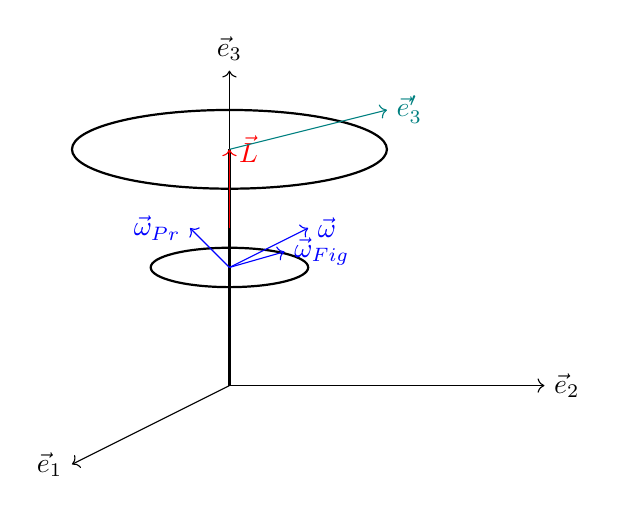
\begin{tikzpicture}
\draw[->] (0,0) -- (4,0) node[right] {$\vec{e}_2$};
\draw[->] (0,0) -- (0,4) node[above] {$\vec{e}_3$};
\draw[->] (0,0) -- (-2,-1) node[left] {$\vec{e}_1$};

\draw[thick] (0,3) ellipse (2cm and 0.5cm);
\draw[thick] (0,0) -- (0,3);
\draw[thick] (0,1.5) ellipse (1cm and 0.25cm);

\draw[->, red] (0,2) -- (0,3) node[right] {$\vec{L}$};
\draw[->, blue] (0,1.5) -- (1,2) node[right] {$\vec{\omega}$};
\draw[->, blue] (0,1.5) -- (-0.5,2) node[left] {$\vec{\omega}_{Pr}$};
\draw[->, blue] (0,1.5) -- (0.7,1.7) node[right] {$\vec{\omega}_{Fig}$};
\draw[->, teal] (0,3) -- (2,3.5) node[right] {$\vec{e}_3^\prime$};
\end{tikzpicture}

\begin{itemize}
\item Da ohne resultierendes Drehmoment $\vec{L}$ = konst, ist im Inertial-System $\vec{\underset{\sim}{L}}$ konstant. Wir können daher die $\vec{e}_3$-Achse so legen dass sie in Richtung von $\vec{\underset{\sim}{L}}$ zeigt.

\item Da $T_{rot} = \frac{1}{2}\vec{\omega}\cdot\vec{L}$ = konst, schließen $\vec{\omega}$ und $\vec{L}$ immer denselben Winkel ein; $\vec{\omega}(t)$ umläuft $\vec{L}$ auf fest stehendem Kreiskegel.

\item Da $\vec{L}$, $\vec{\omega}$, $\vec{e}_3$ in einer Ebene liegen, können wir $\vec{\omega}$ in einen Anteil $\vec{\omega}_{Pr}$ in Richtung $\vec{L}$ zerlegen, und in einen Anteil $\vec{\omega}_{Fig}$ in Richtung der Figurenachse, $\vec{\omega}_{Fig}$:

\[\vec{\omega} = \vec{\omega}_{Pr} + \vec{\omega}_{Fig}\]

$\omega_{Pr}$ = Kreisfrequenz mit welcher die Figurenachse $\vec{e}_1$ und $\vec{\omega}$ den konstanten Drehimpuls umlaufen (Kräftefreie Präzession)

$\omega_{Fig}$ = Kreisfrequenz mit der Körper um seine Figurenachse rotiert.
\end{itemize}

Durch einfache geometrische Überlegungen können wir $\omega_{Pr}$ und $\omega_{Fig}$ durch die Erhaltungsgrößen $L=|\vec{L}|$ und $L_3^\prime$ ausdrücken:

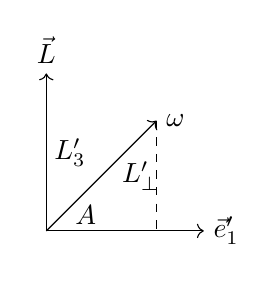
\begin{tikzpicture}
\draw[->] (0,0) -- (2,0) node[right] {$\vec{e}_1^\prime$};
\draw[->] (0,0) -- (0,2) node[above] {$\vec{L}$};
\draw[->] (0,0) -- (1.4,1.4) node[right] {$\omega$};
\draw[dashed] (0,0) -- (1,0);
\draw (0.5,0.2) node {$A$};
\draw[dashed] (1.4,1.4) -- (1.4,0);
\draw (1.2,0.7) node {$L_\perp^\prime$};
\draw (0.3,1) node {$L_3^\prime$};
\end{tikzpicture}

\[\sin \vartheta_L = \frac{L_\perp^\prime}{L} = \frac{A}{\omega_{Pr}} \quad \text{mit} \quad A = \frac{L_\perp^\prime}{I_1^\prime} \Rightarrow \omega_{Pr} = \frac{L}{I_1^\prime} \quad \text{(erhalten!)}\]

Ferner folgt aus der Skizze:

\[\omega_{Fig} = \omega_3^\prime - \omega_{Pr} \cos \vartheta_L\]
\[\cos \vartheta_L = \frac{L_3^\prime}{L}\]

\[\Rightarrow \omega_{Pr} \cos \vartheta_L = \frac{L}{I_1^\prime} \cdot \frac{L_3^\prime}{L} = \frac{L_3^\prime}{I_1^\prime} = \frac{I_3^\prime\omega_3^\prime}{I_1^\prime}\]

\[\Rightarrow \omega_{Fig} = (1-\frac{I_3^\prime}{I_1^\prime})\omega_3^\prime = \frac{I_1^\prime-I_3^\prime}{I_1^\prime}\frac{L_3^\prime}{I_3^\prime} = -\Omega \quad \text{(erhalten!)}\]

Die bei der Beschreibung der Bewegung im körperfesten System relevante Frequenz $\Omega$ ist also bis auf ein Vorzeichen die Rotationsfrequenz um die Figurenachse.


\pagebreak
\printbibliography
\end{document}